\documentclass[
  output=book,
  nonflat,
  modfonts,
  colorlinks,
  smallfont,
  widdowandorphancontrol
]{langsci/langscibook}

\usepackage{makeidx}
\index{Auslautverhärtung|see{Endrand!Desonorisierung}}
\index{Adjektiv!Positiv|see{Komparation}}
\index{Adjektiv!Steigerung|see{Komparation}}
\index{Adjektiv!Superlativ|see{Komparation}}
\index{Adjunkt|see{Angabe}}
\index{Aktiv|see{Passiv}}
\index{Alveolen|see{Zahndamm}}
\index{Anhebungsverb|see{Verb!Halbmodal--}}
\index{Argument|see{Ergänzung}}
\index{Auxiliar|see{Verb!Hilfs--}}
\index{Beiwort|see{Adverb}}
\index{Betonung|see{Akzent}}
\index{Beugung|see{Flexion}}
\index{Bilabial|see{Labial}}
\index{Bindewort|see{Konjunktion}}
\index{Dativ!Commodi|see{Nutznießer--}}
\index{Dativ!Iudicantis|see{Bewertungs--}}
\index{Dativ!Zugehörigkeits--|see{Pertinenz--}}
\index{Deklination|see{Substantiv!Flexion}}
\index{Determinativ|see{Artikelwort}}
\index{Determinierer|see{Artikelwort}}
\index{Diathese|see{Passiv}}
\index{Distribution|see{Verteilung}}
\index{Eigenschaftswort|see{Adjektiv}}
\index{Einzahl|see{Numerus}}
\index{Ergänzungssatz|see{Komplementsatz}}
\index{Fall|see{Kasus}}
\index{Formenlehre|see{Morphologie}}
\index{Futur II|see{Futurperfekt}}
\index{Fürwort|see{Pronomen}}
\index{Genus verbi|see{Passiv}}
\index{Geräuschlaut|see{Obstruent}}
\index{Geschlecht|see{Genus}}
\index{Glottisverschluss|see{Glottalverschluss}}
\index{Glottis|see{Stimmbänder}}
\index{Grammatik!normativ|see{Grammatik!präskriptiv}}
\index{Gruppe|see{Phrase}}
\index{Hauptsatz|see{Satz}}
\index{Hauptwort|see{Substantiv}}
\index{Kernsatz|see{Satz!Verb-Zweit--}}
\index{Klitisierung|see{Klitikon}}
\index{Knalllaut|see{Plosiv}}
\index{Komparativ|see{Adjektiv!Komparation}}
\index{Komplement|see{Ergänzung}}
\index{Komposition|see{Kompositum}}
\index{Konjugation|see{Verb!Flexion}}
\index{Konjunktion!subordinierend|see{Komplementierer}}
\index{Konstantschreibung|see{Schreibprinzip|Konstanz}}
\index{Kopula|see{Verb!Kopula}}
\index{Labiodental|see{Labial}}
\index{Larynx|see{Kehlkopf}}
\index{Mehrzahl|see{Numerus}}
\index{Mitlaut|see{Konsonant}}
\index{Pharynx|see{Rachen}}
\index{Plural|see{Numerus}}
\index{Plusquamperfekt|see{Präteritumsperfekt}}
\index{Reduktionsvokal|see{Schwa}}
\index{Reibelaut|see{Frikativ}}
\index{Rekursivität|see{Rekursion}}
\index{Relation!syntagmatisch|see{Relation!syntaktisch}}
\index{Satzbau|see{Syntax}}
\index{Selbstlaut|see{Vokal}}
\index{Silbe!Coda|see{Endrand}}
\index{Silbe!Nukleus|see{Kern}}
\index{Silbe!Onset|see{Anfangsrand}}
\index{Silbifizierung|see{Silbe}}
\index{Singular|see{Numerus}}
\index{Spannsatz|see{Satz!Verb-Letzt--}}
\index{Stirnsatz|see{Satz!Verb-Erst--}}
\index{Subjunktor|see{Komplementierer}}
\index{Theta-Rolle|see{Rolle}}
\index{Trace|see{Spur}}
\index{Tuwort|see{Verb}}
\index{Uvula|see{Zäpfchen}}
\index{Velum|see{Gaumensegel}}
\index{Vokalviereck|see{Vokaltrapez}}
\index{Vorsilbe|see{Präfix}}
\index{Wortart|see{Wortklasse}}
\index{Wortform|see{Wort!syntaktisches}}
\index{Zeitform|see{Tempus}}
\index{Zeitwort|see{Verb}}
\index{glottal stop|see{Glottalverschluss}}
\index{grammatisch|see{Grammatikalität}}
\index{ungrammatisch|see{Grammatikalität}}
\index{Hypotaxe|see{Parataxe und Hypotaxe}}
\index{Funktion|see{Form und Funktion}}
\index{Fugenelement|see{Kompositum!Fugenelement}}

\makeindex

\title{Einführung in die grammatische Beschreibung des Deutschen}
\subtitle{Dritte, überarbeitete und erweiterte Auflage}
\BackTitle{Einführung in die grammatische Beschreibung des Deutschen}
\BackBody{\begin{sloppypar}
\textit{Einführung in die grammatische Beschreibung des Deutschen} ist eine Einführung in die Grammatik des gegenwärtigen Deutschen in den Bereichen Phonetik, Phonologie, Morphologie, Syntax und Graphematik.
Das Buch ist für alle geeignet, die sich für die Grammatik des Deutschen interessieren, vor allem aber für Studierende der Germanistik bzw.\ Deutschen Philologie, insbesondere auch für Lehramtsstudierende.
Im Vordergrund steht die Vermittlung grammatischer Erkenntnisprozesse und Argumentationsweisen auf Basis konkreten sprachlichen Materials.
Es wird kein spezielles theoretisches Modell angenommen, aber alle, die das Buch gelesen haben, sollten in der Lage sein, sowohl deskriptiv ausgerichtete Forschungsartikel als auch theorienahe Einführungen lesen zu können.
Das Buch enthält zahlreiche Übungsaufgaben, die im Anhang gelöst werden.

Die dritte Auflage behebt Tipp- und Stilfehler und bietet einige neue Vertiefungsblöcke sowie eine komplette Überarbeitung der Grafiken und Diagramme.
Ein Kapitel über Grammatik in Schule und Lehramtsstudium ergänzt das Buch.

\vspace{1\baselineskip}

\noindent\textbf{Roland Schäfer} ist Germanist und Linguist.
Er hat an der Phi\-lipps-\-Universität Marburg studiert und war wissenschaftlicher Mitarbeiter an der Georg-August Universität Göttingen und der Freien Universität Berlin.
Er hat Professuren in Göttingen (2011\slash 2012) und an der Freien Universität Berlin (2016 und seit 2018) vertreten.
Nach seiner Promotion in Göttingen im Jahr 2008 hat er 2018 eine Habilitationsschrift zum Thema \textit{Probabilistic German Morphosyntax} (eine Analyse von sogenannten \textit{Zweifelsfällen} im Rahmen der probabilistischen Grammatik) vorgelegt, auf Basis derer die Humboldt-Universität zu Berlin sein Habilitationsverfahren zur Erlangung der Venia legendi für germanistische und allgemeine Sprachwissenschaft eröffnet hat.
Seine aktuellen Forschungsschwerpunkte sind die probabilistische Morphosyntax und Graphematik des Deutschen, empirische und statistische Verfahren, Fachdidaktik und Lehramtsausbildung sowie die Korpuserstellung.
Von 2015 bis 2018 leitete er erfolgreich das selber eingeworbene DFG-Projekt \textit{Linguistische Web-Charakterisierung und Webkorpuserstellung} an der Freien Universität Berlin.
\end{sloppypar}
}

\dedication{%
\large Für Adrianna, Alma, Ariel, Block, Frau Brüggenolte, Chloe, Chopin, Christina, Doro, Edgar, Elena, Elin, Emma, den ehemaligen FCR Duisburg, Frida, Gabriele, Hamlet, Helmut Schmidt, Henry, Ian Kilmister, Ingeborg, Ischariot, Jean-Pierre, Johan, Juliette, Kiki, Kristine, Kurt, Lemmy, Liv, Marina, Martin, Mats, Mausi, Michelle, Nadezhda, Herrn Oelschlägel, Oma, Opa, Pavel, Philly, Sarah, Scully, Stig, Tania, Tante Klärchen, Tarek, Tatjana, Herrn Uhl, Ullis schreckhaften Hund, Vanessa und so.\\[\baselineskip]Wenn das schonmal klar sein würde.\\}

\typesetter{Roland Schäfer}

\proofreader{Thea Dittrich, Luise Rißmann, Ulrike Sayatz (in alphabetical order)}

\author{Roland Schäfer}

\BookDOI{10.5281/zenodo.1421660}
\renewcommand{\lsISBNdigital}{978-3-96110-116-0}
\renewcommand{\lsISBNhardcover}{978-3-96110-117-7}
\renewcommand{\lsISBNsoftcover}{978-3-96110-118-4}
\renewcommand{\lsISBNsoftcoverus}{978-1727793741}
\renewcommand{\lsSeries}{tbls}
\renewcommand{\lsSeriesNumber}{2}
\renewcommand{\lsURL}{http://langsci-press.org/catalog/book/224}

 
 
 
 
  

\usepackage{graphicx}
\usepackage{tabularx}
\usepackage{multicol}

% RS langsci

\usepackage{./langsci/styles/langsci-optional}
\usepackage{./langsci/styles/langsci-gb4e}
\usepackage{./langsci/styles/langsci-lgr}
\usepackage{./langsci/styles/langsci-glyphs}
\usepackage{./langsci/styles/langsci-tbls}
\usepackage[linguistics]{forest}

% RS only for editing.
% \usepackage{soul}

% RS

\usepackage{unicode-math}
\usepackage{fontspec}

\usepackage{setspace}
\usepackage{cancel}
\let\B\relax
\let\T\relax
\usepackage{xcolor}
\usepackage{colortbl}
\usepackage{multirow}
\usepackage{verbatim}
\usepackage{enumitem}
\usepackage{ifthen}
\usepackage{float}
\usepackage{savesym}
\savesymbol{iint}
\savesymbol{iiint}
\usepackage{amsmath}
\restoresymbol{TXF}{iint}
\restoresymbol{TXF}{iiint}
\usepackage{rotating}
\usepackage{boxedminipage}
\usepackage{tocloft}
\usepackage{etoolbox}
\usepackage{pifont}

\usepackage{xeCJK}
\setCJKmainfont{MS Mincho}
\setCJKsansfont{MS Gothic}

\usepackage{tikz}
\usetikzlibrary{positioning,arrows.meta,cd}
\tikzset{>=latex}


%% hyphenation points for line breaks
%% Normally, automatic hyphenation in LaTeX is very good
%% If a word is mis-hyphenated, add it to this file
%%
%% add information to TeX file before \begin{document} with:
%% %% hyphenation points for line breaks
%% Normally, automatic hyphenation in LaTeX is very good
%% If a word is mis-hyphenated, add it to this file
%%
%% add information to TeX file before \begin{document} with:
%% %% hyphenation points for line breaks
%% Normally, automatic hyphenation in LaTeX is very good
%% If a word is mis-hyphenated, add it to this file
%%
%% add information to TeX file before \begin{document} with:
%% \include{localhyphenation}
\hyphenation{
Pho-nem
Pho-ne-me
Pho-nems
Pho-ne-men
No-mi-nal-phra-se
Mo-no-fle-xi-on
Verb-par-ti-kel
Verb-kom-plex
Ar-ti-ku-la-tion
Rechts-att-ri-bu-te
Verb-par-ti-kel
Verb-par-ti-keln
Lexi-kon
Verb-phra-se
Verb-kom-plex}


\hyphenation{
Pho-nem
Pho-ne-me
Pho-nems
Pho-ne-men
No-mi-nal-phra-se
Mo-no-fle-xi-on
Verb-par-ti-kel
Verb-kom-plex
Ar-ti-ku-la-tion
Rechts-att-ri-bu-te
Verb-par-ti-kel
Verb-par-ti-keln
Lexi-kon
Verb-phra-se
Verb-kom-plex}


\hyphenation{
Pho-nem
Pho-ne-me
Pho-nems
Pho-ne-men
No-mi-nal-phra-se
Mo-no-fle-xi-on
Verb-par-ti-kel
Verb-kom-plex
Ar-ti-ku-la-tion
Rechts-att-ri-bu-te
Verb-par-ti-kel
Verb-par-ti-keln
Lexi-kon
Verb-phra-se
Verb-kom-plex}


\bibliography{localbibliography}

% \includeonly{chapters/phonetik}

\begin{document}

% By LSP.
\renewbibmacro*{index:name}[5]{%
  \usebibmacro{index:entry}{#1}
    {\iffieldundef{usera}{}{\thefield{usera}\actualoperator}\mkbibindexname{#2}{#3}{#4}{#5}}}


% By LSP.
\makeatletter
\def\blx@maxline{77}
\makeatother


% Mark for proof-reading/revision.
\newcommand{\Dirty}{\marginpar{\hl{DIRTY!}}}


% Fix line spacing in list environmens.
\setlist{noitemsep}


% Correct hyperref colors. The original ones would give you eye cancer.
\hypersetup{
  linkbordercolor  = {white}
%  , linkcolor        = {lsMidDarkBlue}
%  , anchorcolor      = {lsMidWine}
%  , citecolor        = {lsDarkGreenOne}
%  , menucolor        = {lsMidDarkBlue}
%  , urlcolor         = {lsDarkOrange}
%    , filecolor       = {}
%    , runcolor        = {}
}


% Use a better mono font, ideal for code.
% https://github.com/chrissimpkins/codeface/tree/master/fonts/inconsolata-g
% \setmonofont{Inconsolata-g}


% Use a math font that actually works! Requires unicode-math paackage.
% https://github.com/khaledhosny/libertinus
\setmathfont[Scale=MatchUppercase]{libertinusmath-regular.otf}


\newenvironment{listLileveli}{\begin{enumerate}}{\end{enumerate}}
\newenvironment{listLilevelii}{\begin{enumerate}}{\end{enumerate}}
\newenvironment{listLileveliii}{\begin{enumerate}}{\end{enumerate}}
\newenvironment{listLileveliv}{\begin{enumerate}}{\end{enumerate}}
\newenvironment{listLiileveli}{\begin{itemize}}{\end{itemize}}
\newenvironment{listLiilevelii}{\begin{itemize}}{\end{itemize}}
\newenvironment{listLiileveliii}{\begin{itemize}}{\end{itemize}}
\newenvironment{listLiileveliv}{\begin{itemize}}{\end{itemize}} 

% define own variables for hacks
\newlength{\myBuffer}

% formatting
\newcommand{\Lf}{
  \setlength{\itemsep}{1pt}
  \setlength{\parskip}{0pt}
  \setlength{\parsep}{0pt}
}

% Feinsatz 

\newcommand{\Stretch}[1][1]{\vspace{#1\baselineskip}}
\newcommand{\Unstretch}[1][0.5]{\vspace{-#1\baselineskip}}
\newcommand{\Hardstretch}[1][1]{\vspace*{#1\baselineskip}}
\newcommand{\Enl}[1][1]{\enlargethispage{#1\baselineskip}}
\newcommand{\Np}{\newpage}

% Uncomment to switch off
%\renewcommand{\Stretch}[1][1]{}
%\renewcommand{\Unstretch}[1][0.5]{}
%\renewcommand{\Hardstretch}[1][1]{}
%\renewcommand{\Enl}[1][1]{}
%\renewcommand{\Np}{}


% all sorts of shortcuts
\newcommand{\HStrut}[1]{\rule{0pt}{#1pt}}
\newcommand{\VStrut}[1]{\rule{#1pt}{0pt}}
\newcommand{\Sw}[1]{\begin{sideways}#1\end{sideways}}
\newcommand{\Ast}{*}
\definecolor{lg}{rgb}{.8,.8,.8}
\newcommand{\Dim}{\cellcolor{lg}}
\newcommand{\Tidx}[1]{\ensuremath{_{\mathnormal{#1}}}}
\newcommand{\Rollen}[1]{\ensuremath{\langle}#1\ensuremath{\rangle}}
\newcommand{\Qc}[1]{\texttt{#1}}
\newcommand{\acr}[1]{{#1}}
\newcommand{\ak}[1]{#1\marginpar{\textcolor{textblue}{\footnotesize #1}}}
\newcommand{\mar}[1]{\marginpar{\textcolor{textblue}{\footnotesize #1}}}
\newcommand{\zB}{z.\thinspace{}B.~}
\newcommand{\oA}{o.\thinspace{}ä.~}
\newcommand{\idR}{i.\,d.\,R.\ }
\newcommand{\BBel}[1]{\B[-5]{#1}}
\newcommand{\Bewegtes}[1]{\ensuremath{_{\textrm{#1}}}}
\newcommand{\ORi}{\Bewegtes{1}}
\newcommand{\ORii}{\Bewegtes{2}}
\newcommand{\ORiii}{\Bewegtes{3}}
\newcommand{\ORiv}{\Bewegtes{4}}
\newcommand{\ORv}{\Bewegtes{5}}
\newcommand{\Spur}[1]{t\Sub{#1}}
\newcommand{\Ti}{\Spur{1}}
\newcommand{\Tii}{\Spur{2}}
\newcommand{\Tiii}{\Spur{3}}
\newcommand{\Tiv}{\Spur{4}}
\newcommand{\Akz}{ˈ}
\newcommand{\Nakz}{ˌ}
\newcommand{\PhPr}[1]{\ensuremath{\stackrel{\textnormal{#1\ }}{\Longrightarrow}}}
\newcommand{\phopro}{\ensuremath{\Rightarrow}}

\newcommand{\KTArr}[1]{\ding{226}~\textit{#1}~\ding{226}}

\newcommand{\VfTest}{\KTArr{VfTest}~}
\newcommand{\PronTest}{\KTArr{PronTest}~}
\newcommand{\KoorTest}{\KTArr{KoorTest}~}
\newcommand{\onestar}{◆◇◇}
\newcommand{\twostar}{◆◆◇}
\newcommand{\tristar}{◆◆◆}
\newcommand{\RPr}{\ensuremath{\ll}}
\newcommand{\RUn}{\ensuremath{\sim}}
\newcommand{\REq}{\ensuremath{=}}
\newcommand{\Opsional}{★~}
\newcommand{\Nono}{---}
\newcommand{\Sub}[1]{\ensuremath{_{\text{#1}}}}
\newcommand{\Up}[1]{\ensuremath{^{\text{#1}}}}
\newcommand{\UpSub}[2]{\ensuremath{^{\text{#1}}_{\text{#2}}}}
\newcommand{\TuBegin}{\ding{217}}
\newcommand{\TuEnd}{}
\newcommand{\Folgt}{\ding{217}}

\newcommand*\circlearound[1]{\tikz[baseline=(char.base)]{\node[shape=circle,draw,inner sep=2pt] (char) {#1};}}


% boxes and stuff for definitions, axioms etc.
\definecolor{textblue}{rgb}{0,0,.5}
\definecolor{textred}{rgb}{.5,0,0}
\definecolor{textgreen}{rgb}{0,.5,0}
\definecolor{lightblue}{rgb}{.9,.9,1}
\definecolor{lightgreen}{rgb}{.9,1,.9}
\definecolor{lightred}{rgb}{1,.9,.9}
\definecolor{lightyellow}{rgb}{1,1,.8}
\definecolor{lightgray}{rgb}{.88,.88,.88}
\definecolor{lsLightgray}{gray}{0.88}
\definecolor{lsYellow}{cmyk}{0,0.25,1,0}

\newcommand{\whyte}[1]{\textcolor{white}{#1}}

% bookkeeping of own environments for definitions etc.
\newlistof[chapter]{dgdef}{dgd}{Verzeichnis der Definitionen}
\newlistof[chapter]{dgsatz}{dgs}{Verzeichnis der Sätze}
\newlistof[chapter]{dgvertief}{dgv}{Verzeichnis der Vertiefungen}

\newcounter{deskgram-ziel}
\newcounter{deskgram-ex}
\newcounter{deskgram-strsch}
\newcounter{deskgram-wfilt}
\newcounter{deskgram-pholproz}


% Fix spacing between numbers and caption in list of figures etc.
\makeatletter
  \renewcommand*\l@figure{\@dottedtocline{1}{1em}{3.2em}}
  \renewcommand*\l@table{\@dottedtocline{1}{1em}{3.2em}}
  \renewcommand*\l@dgdef{\@dottedtocline{1}{1em}{3.2em}}
  \renewcommand*\l@dgsatz{\@dottedtocline{1}{1em}{3.2em}}
\makeatother


% NEW Vertiefung (non-floating)

\newcommand{\tblsthickline}{{\color{gray}\rule{\textwidth}{1.5mm}}}

\newenvironment{Sandwich}[1]
  {
    \par\vspace{5mm}\noindent\tblsthickline
    {\par\vspace{3mm}\noindent\sffamily\large\bfseries#1\vspace{4mm}}
  }
  {\par\vspace{3mm}\noindent\tblsthickline\par\vspace{5mm}}


\newenvironment{Vertiefung}[1]
  { 
    \refstepcounter{dgvertief}
    \begin{Sandwich}{#1\hfill Vertiefung~\thechapter.\arabic{dgvertief}}
  }
  {\end{Sandwich}}


% if not using hyperref, redefine this as empty:
\newcommand{\Phantom}{\phantomsection}


\newcommand{\Definition}[2]{
  \refstepcounter{dgdef}
  \tblscolorbox[report]{lsLightGray}{#1\hfill Definition~\thechapter.\arabic{dgdef}}{#2}
}



\newcommand{\Satz}[2]{
  \refstepcounter{dgsatz}
  \tblscolorbox[glass]{lsLightGray}{#1\hfill Satz~\thechapter.\arabic{dgsatz}}{#2}
}



\newcommand{\Zusammenfassung}[1]{
  \tblsframebox[refresh]{lsYellow}{Zusammenfassung von Abschnitt~\thesection}{#1}
}



\newcommand{\WFiltTree}[7][0mm]{%
  \refstepcounter{deskgram-wfilt}
  \tblscolorbox[filter]{lsLightGray}{#2\hfill Wortklassenfilter~\arabic{deskgram-wfilt}}{
    \label{#3}
    \hspace{-5pt}\centering
    \begin{tikzpicture}[baseline]
    \node at (0,0) (Wort) [align=left] {#4};
    \node [right=of Wort.east, text width=3.5cm, align=left] (Filter) {#5};
    \node [above right=\baselineskip and 1cm of Filter.east] (Ja) {#6};
    \node [below right=\baselineskip and 1cm of Filter.east] (Nein) {#7}; 
    \path (Wort) edge [-{Latex[round]}] (Filter);
    \path (Filter.east) edge [-{Latex[round]}] node [above,sloped] {Ja} (Ja.west);
    \path (Filter.east) edge [-{Latex[round]}] node [below,sloped] {Nein} (Nein.west);
    \aeundefinethesenodes{Wort, Filter, Ja, Nein}
  \end{tikzpicture}\vspace{#1}%
  }
}

\newcommand{\strschemspace}{\hspace{1em}}
\newcommand{\Phrasenschema}[2]{
  \refstepcounter{deskgram-strsch}
  \tblscolorbox[tree]{lsLightGray}{#1\hfill Phrasenschema~\arabic{deskgram-strsch}}{
    \centering
    #2
  }
}



% OLD "further reading"
\newcommand{\WeitereLiteratur}[1]{
  \tblsframebox[book]{lsLightGray}{Weiterführende Literatur zu \thepart}{#1}
}


% Excercises.
\newcounter{Exer}[chapter]

\newcommand{\Uebung}[2][\twostar]{%
  \par\medskip\refstepcounter{Exer}\noindent\textbf{Übung~\arabic{Exer}}~#1\ %
  \ifthenelse{\equal{#2}{}}
  {}
  {(Lösung auf Seite \pageref{sol:#2})\ }
}

\newcommand{\Uebungen}{
  \clearpage
  \section*{Übungen zu Kapitel \thechapter}
  \markboth{Übungen zu Kapitel \thechapter}{Übungen zu Kapitel \thechapter}
  \setcounter{equation}{0}
}

\newcommand{\Loesungen}[2][\clearpage]{#1\section*{Zu Kapitel \ref{#2}}}
\newcommand{\Loesung}[1]{\subsection*{Übung \ref{exc:#1} (Seite \pageref{exc:#1})}}

\renewcommand{\Phantom}{}


%%%%%%%%%%%%%%%%%%%%%%%%%%%%%%%%%%%%%%
% Text used in more than one chapter %
%%%%%%%%%%%%%%%%%%%%%%%%%%%%%%%%%%%%%%

\newcommand{\DefWort}{Das (\textit{lexikalische}) \textit{Wort} ist eine Repräsentation von paradigmatisch zusammengehörenden Wortformen.
Umgangssprachlich kann man von der Zusammenfassung aller möglichen Formen eines Wortes sprechen.
Für das lexikalische Wort sind die Werte nur für diejenigen Merkmale spezifiziert, die in allen Wortformen des Paradigmas dieselben Werte haben.
Die restlichen Werte werden gemäß der Position im Paradigma bei den konkret vorkommenden Wortformen des Wortes gesetzt.}

\newcommand{\ThePhrasenExOne}{dass [[dem Jungen] [die Mutter] [ein Eis] [geschenkt hat]]}
\newcommand{\ThePhrasenExTwo}{dass [[ein Eis] [die Mutter] [dem Jungen] [geschenkt hat]]}


%%%%%%%%%%%%
%%% TikZ %%%
%%%%%%%%%%%%

% Undefining node names.

\makeatletter

\long\def\ifnodedefined#1#2#3{%
  \@ifundefined{pgf@sh@ns@#1}{#3}{#2}}

\newcommand\aeundefinenode[1]{%
  \expandafter\ifx\csname pgf@sh@ns@#1\endcsname\relax
  \else
    \typeout{Undefining node "#1"}%
    \global\expandafter\let\csname pgf@sh@ns@#1\endcsname\relax
  \fi
}

\newcommand\aeundefinethesenodes[1]{%
  \foreach \myn  in {#1}
    {%
      \ifnodedefined{\myn}{%
      \expandafter\aeundefinenode\expandafter{\myn}%
    }{}
    }%
}

\newcommand\aeundefinenumericnodes{%
  \foreach \myn in {1,2,...,50}
    {%
      \ifnodedefined{\myn}{%
      \expandafter\aeundefinenode\expandafter{\myn}%
    }{}
    }%
}
\makeatother

% Drawing sonority diagrams.

\newcommand{\plo}{0}
\newcommand{\fri}{0.5}
\newcommand{\nas}{1}
\newcommand{\liq}{1.5}
\newcommand{\vok}{2}

% Save text.
\newcommand{\lastsaved}{}
\newcommand{\textsave}[1]{\gdef\lastsaved{#1}#1}

\newcommand{\SonDiag}[2][0]{%
  \begin{tikzpicture}
    \textsave{.}
    \tikzset{
      normalseg/.style={fill=white},
      extrasyll/.style={circle, draw, fill=white},
      sylljoint/.style={diamond, draw, fill=white}
    }
    \node at (0,\plo) {P};
    \node at (0,\fri) {F};
    \node at (0,\nas) {N};
    \node at (0,\liq) {L};
    \node at (0,\vok) {V};

    % Draw the helper lines if required.
    \ifthenelse{\equal{#1}{0}}{}{%
      \foreach \y in {\plo, \fri, \nas, \liq,\vok} {%
	\draw [dotted, |-|] (0.25, \y) -- (#1.75, \y);
      }
    }

    \foreach [count=\x from 1, remember=\x as \lastx] \p / \y / \g in #2 {
      \ifthenelse{\equal{\y}{-1}}{\textsave{.}}{%

	% Draw the node, either plain, as Silbenbgelenk, or as extrasyllabic.
        \ifthenelse{\equal{\g}{1}}{%
	  \node (\x) [sylljoint] at (\x, \y) {\p};
	}{%
	  \ifthenelse{\equal{\g}{2}}{%
	    \node (\x) [extrasyll] at (\x, \y) {\p};
	  }{%
	    \node (\x) [normalseg] at (\x, \y) {\p};
	  }
	}

	% Draw the connection unless the previous node was not or was empty.
	\ifthenelse{\NOT\equal{\lastsaved}{.}}{%
	  \draw [->] (\lastx) to (\x);
	}{}
	\textsave{1}
      }
    }
    \aeundefinenumericnodes
  \end{tikzpicture}
}

\forestset{
  Ephr/.style={draw, ellipse, thick, inner sep=2pt},
  Eobl/.style={draw, rounded corners, inner sep=5pt},
  Eopt/.style={draw, rounded corners, densely dashed, inner sep=5pt},
  Erec/.style={draw, rounded corners, double, inner sep=5pt},
  Eoptrec/.style={draw, rounded corners, densely dashed, double, inner sep=5pt},
  Ehd/.style={rounded corners, fill=gray, inner sep=5pt,
    delay={content=\whyte{##1}}
  },
  Emult/.style={for children={no edge}, for tree={l sep=0pt}},
  phrasenschema/.style={for tree={l sep=2em, s sep=2em}},
  decide/.style={draw, chamfered rectangle, inner sep=2pt},
  finall/.style={rounded corners, fill=gray, text=white},
  intrme/.style={draw, rounded corners},
  yes/.style={edge label={node[near end, above, sloped, font=\scriptsize]{Ja}}},
  no/.style={edge label={node[near end, above, sloped, font=\scriptsize]{Nein}}},
  sake/.style={tier=preterminal},
  ake/.style={
    tier=preterminal
    },
}



%%%%%%%%%%
% forest %
%%%%%%%%%%

\forestset{
  narroof/.style={roof, inner xsep=-0.25em, rounded corners},
}


\maketitle
\frontmatter

\currentpdfbookmark{Inhalt}{name}
\tableofcontents

\Phantom
\addcontentsline{toc}{part}{Vorbemerkungen zur ersten Auflage}


\chapter*{Vorbemerkungen zur ersten Auflage}
\markboth{Vorbemerkungen zur ersten Auflage}{Vorbemerkungen zur ersten Auflage}

\section*{Über dieses Buch}

Typische Leser dieser Einführung sind Studierende der Germanistik bzw.\ der Deutschen Philologie, die sich vor dem Studium oder währenddessen einen Überblick über wichtige grammatische Phänomene des Deutschen verschaffen möchten.%
\footnote{Im gesamten Buch wird das generische Maskulinum (\textit{Leser}, \textit{Sprecher}, \textit{Hörer} usw.) verwendet.
Als grammatische Form soll es dabei immer Personen aller Gender bezeichnen.}
Darüber hinaus ist dieses Buch für jeden geeignet, der sich für die deutsche Sprache und ihre Grammatik interessiert.
Eine sehr gute (erstsprachliche oder nahezu erstsprachliche) Kenntnis des Deutschen ist dabei angesichts der Anlage des Buchs von Vorteil.
Es ist also kein ideales Buch für all jene, die Deutsch lernen wollen und dabei noch nicht sehr weit fortgeschritten sind.

Man kann sich nun die Frage stellen, warum man überhaupt eine Einführung in die Grammatik einer Sprache benötigt, die man bereits sehr gut (ggf.\ sogar als Erstsprache) beherrscht.
Es gibt mehrere Antworten auf diese Frage.
Einerseits ist die Beschäftigung damit, wie wir Sprache benutzen, warum und wozu wir das tun, und wie die Sprache genau beschaffen ist, von grundlegendem Interesse.
Die Linguistik betreibt sozusagen in vielen Bereichen Grundlagenforschung.
Das Interesse für diese grundlegenden Fragen ist ein guter Grund, sich die eigene Sprache, die man täglich meist ohne große Reflexion benutzt, einmal analytisch und genau anzusehen.

Andererseits reden Menschen oft und gerne über die Grammatik ihrer eigenen Sprache -- nicht nur, aber natürlich besonders häufig, wenn die Frage nach dem \textit{richtigen Sprachgebrauch} aufkommt.
Gerade Studierende und Lehrende der Germanistik sollten von Berufs wegen in der Lage sein, an solchen Diskursen informiert teilzunehmen.
Dabei ist es hilfreich, zu wissen, was im System der Grammatik die Zusammenhänge (\zB zwischen Formenbildung und Satzbau) sind, was die Regeln und was die Ausnahmen sind.
Schon die Frage, warum es denn \textit{ein roter Ballon} aber \textit{der rote Ballon} heißt, ist nicht trivial zu beantworten, denn immerhin lautet es einmal \textit{roter} und einmal \textit{rote}, obwohl es sich doch in beiden Fällen um einen Nominativ Singular Maskulinum handelt.
Der Bedarf an einem guten Überblick über die Grammatik wird größer, wenn typische Berufsfelder für Germanisten ins Auge gefasst werden, \zB der Lehrberuf an Schulen, die Fremdsprachendidaktik oder das Verlagswesen.
Gerade wenn es darum geht, anderen Menschen zu vermitteln, wie bestimmte Dinge auf Deutsch gesagt oder geschrieben werden, oder darum, Texte anderer Personen grammatisch zu überprüfen, kann man sich nicht einfach darauf zurückziehen, dass man ja selber weiß, wie es richtig heißt.
Es entsteht der Bedarf an einer \textit{Erklärung}.

Daher wird in dieser Einführung ein Überblick über die wichtigen grammatischen Phänomene des Deutschen gegeben.
Gleichzeitig wird vermittelt, wie man Laute, Buchstaben, Wörter und Sätze einer Sprache, die man bereits beherrscht, so in ein System bringen kann, dass man mit anderen darüber reden kann.
Es geht sozusagen darum, aus sprachlichem Material die Regeln und die Ausnahmen zu den Regeln zu extrahieren und sie uns bewusst zu machen.
Ohne Vorkenntnisse durch bloßes Nachdenken in vertretbarer Zeit Fragen wie die folgenden präzise zu beantworten, ist vergleichsweise schwer:
Wieviele und welche Silben hat das Deutsche?
Warum gibt es Wörter wie \textit{bohrt}, aber prinzipiell keine Wörter wie \textit{bohrp}?
Was sind die typischen Betonungsmuster der Wörter?
Wie kann man am einfachsten beschreiben, wie bei Nomina der Kasus markiert wird?
Warum gibt es überhaupt verschiedene Kasus?
Was ist der Unterschied zwischen starken und schwachen Verben?
Nach welchen Regeln funktioniert die Satzgliedstellung im Deutschen?
Welche Verben kann man ins Passiv setzen?
Schreiben wir so, wie wir sprechen?
Warum gibt es in der deutschen Schrift doppelte Konsonanten?
Was ist die Funktion der Satzzeichen?

Dieses Buch ergänzt andere Literatur, die oft im Studium eingesetzt wird, oder bereitet auf diese vor.
Anspruchsvolle Grammatiken wie der \textit{Grundriss der deutschen Grammatik} von Peter Eisenberg \citep{Eisenberg2013a,Eisenberg2013b} oder die Duden"=Grammatik \citep{Duden8} werden durch die Lektüre dieses Buchs besser lesbar, weil große Teile der grammatischen Terminologie bereits bekannt sind, und weil der Umgang mit sprachlichem Material bereits kleinteiliger geübt wurde, als es in wissenschaftlichen Grammatiken möglich und zielführend ist.
Hat man einen solchen Überblick nicht, kann es bereits Schwierigkeiten bereiten, in umfangreichen Grammatiken wie der Duden-Grammatik den richtigen Abschnitt zu einer konkreten grammatischen Fragestellung zu finden.
Einführungen, die einen Überblick über viele Teildisziplinen der germanistischen Linguistik geben -- \zB \citet{MeibauerEa2007, SteinbachEa2007} --, oder Einführungen in spezifische Grammatiktheorien -- \zB \citet{Grewendorf2002, Mueller2008, Sternefeld2008, Sternefeld2009} -- sind nach der Lektüre dieser Einführung besser verständlich, da grammatische Kategorien detailliert an konkretem Material bereits erklärt wurden und dadurch auf andere Phänomene, andere Teilbereiche der Linguistik oder formalere Theorien bezogen werden können.

\section*{Benutzung dieses Buchs}

Das Buch ist für einen primären Arbeitszyklus \textit{Lesen--Unterrichten--Üben} konzipiert.
Das Gelesene soll durch den Unterricht gefestigt werden, die wichtigsten Punkte dabei herausgestellt werden und Probleme und Fragen erörtert werden.
Die in kurzen Sätzen gehaltenen Zusammenfassungen am Ende jedes Kapitels sollen vor allem eine Gedächtnisstütze zwischen dem Lesen und dem Unterrichten sein.

Praxis in der Anwendung der beschriebenen Analyseverfahren kann durch die zahlreichen Übungen im Anschluss an die Kapitel erworben werden.
Die Übungen zu den einzelnen Kapiteln werden fast alle im Anhang gelöst.%
\footnote{Anmerkung zur zweiten Auflage:
Der Anteil der Aufgaben, für die eine Lösung angeboten wird, ist in der zweiten Auflage rückläufig, insbesondere bei Transferaufgaben.
Auch wenn dies für das Selbststudium evtl.\ ungünstig ist, ist es für die Arbeit im Seminar zuträglich.}
Dadurch wird es im Selbststudium ermöglicht, den eigenen Lernerfolg zu kontrollieren.
Das Niveau der Übungen wird dabei durch \onestar\ (einfache Übungen), \twostar\ (Übungen auf Klausurniveau) und \tristar\ (Transferaufgaben) gekennzeichnet.

Bezüglich der Unterscheidung von hervorgehobenen Definitionen und Sätzen gilt, dass Definitionen für den argumentativen Gesamtaufbau grundlegend sind, während Sätze nur hilfreiche Schlussfolgerungen, nicht-definierende Eigenschaften und Tendenzen usw.\ formulieren.

Mit fortgeschrittenen Argumentationen bzw.\ interessanten, aber in der gegebenen Situation weniger zentralen Informationen wird folgendermaßen verfahren:
Bis zu einer Länge von ungefähr drei Sätzen werden sie in Fußnoten gesetzt.
Darüber hinaus und bis zu einer Länge von ungefähr einer Seite werden sie in deutlich abgesetzte Vertiefungsblöcke gesetzt.
Noch längere Vertiefungen werden als optionale Abschnitte des Textes gesetzt und sind im Titel mit \Opsional markiert.%
\footnote{Anmerkung zur zweiten Auflage:
Es gibt jetzt nur noch ein einheitliches Format für vertiefende Abschnitte.}
Das Buch kann auch selektiv gelesen werden, zumal wenn ein bisschen Hin- und Herblättern zwischen den Kapiteln in Kauf genommen wird.
Besonders die fünf Teile sind sehr gut einzeln lesbar.

Die Abschnitte mit weiterführender Literatur am Ende jedes der fünf Teile des Buchs stellen keine exhaustive Bibliographien dar.
Es werden spezialisierte Einführungen und exemplarisch einige (möglichst gut lesbare und möglichst auf Deutsch verfasste) Fachartikel und Monographien genannt, die interessierten Lesern den weiteren Einstieg in die Lektüre wissenschaftlicher Primärtexte ermöglichen sollen.%
\footnote{Leser sollten damit rechnen, dass in den angeführten Werken ggf.\ andere Positionen als in diesem Buch vertreten werden.}
Im Text wird aus Gründen der Übersichtlichkeit nur in Einzelfällen auf weitere Literatur verwiesen, \zB wenn nicht-triviale Beispiele, Listen, Paradigmen usw.\ direkt aus anderen Werken übernommen wurden.

\section*{Danksagungen zur ersten Auflage}

Ich möchte zunächst den Initiatoren und Unterstützern von Language Science Press, den Reihenherausgebern -- Martin Haspelmath und Stefan Müller -- sowie Sebastian Nordhoff als Koordinator von Language Science Press dafür danken, dass sie die Bedingungen dafür geschaffen haben, dass das Buch als Open-Access-Publikation erscheinen kann.
Stefan Müller danke ich darüber hinaus für eine sehr gründliche Durchsicht und eine Fülle von Kommentaren und Anmerkungen, die erheblich zur Verbesserung des Buchs beigetragen haben.
Besonderer Dank gilt Eric Fuß, der als Gutachter nicht nur einem offenen Begutachtungsprozess zugestimmt hat, sondern auch zahlreiche Anmerkungen und Kommentare gegeben hat, die ich fast vollständig übernehmen konnte.

Weiterhin danke ich den Teilnehmern und Tutorinnen meiner Lehrveranstaltungen an der Freien Universität Berlin in den Jahren 2008--2014, die viel Rückmeldung zu früheren Versionen des Textes gegeben haben.
Insbesondere sind zu nennen (in alphabetischer Reihenfolge) Sarah Dietzfelbinger, Ana Draganovi\'{c}, Lea Helmers, Theresia Lehner, Kaya Triebler, Samuel Reichert, Johanna Rehak, Cynthia Schwarz, Jana Weiß.
Für ihre Hilfe bei der Endredaktion in letzter Minute danke ich Kim Maser.
Für ausführliche Kommentare zu diversen Fassungen danke ich (in alphabetischer Reihenfolge) Götz Keydana, Michael Job, Bjarne Ørsnes, Ulrike Sayatz, Julia Schmidt, Nicolai Sinn.
Götz danke ich auch besonders für sie slawischen Beispiele, Nicolai besonders für die Diskussionen und Anregungen zu Kapitel~\ref{sec:nominalflexion}.
Ulrike danke ich vor allem für kontroverse Diskussionen zur und Nachhilfe in Graphematik, ohne die ich Teil~\ref{part:schrift} nicht hätte schreiben können.
Bjarne und Nicolai waren wichtige moralische Unterstützer und inhaltliche Ratgeber in der Frühphase des Projektes.
Felix Bildhauer danke ich für die Zusammenstellung der \textit{Außenseiter}-Sätze in Kapitel~\ref{sec:grammatik} (S.\ \pageref{ex:dg9113}).

Beim Redigieren des fertigen Buchs leuchtete Thea Dittrich.

Für alle Fehler und Inadäquatheiten, die jetzt noch im Buch verblieben sind, trage ich die alleinige Verantwortung.
Ich hätte eben besser auf all die oben genannten Personen hören sollen.

Für eine prägende Einführung in deskriptive grammatische Analysen und Argumentationen möchte ich bei dieser Gelegenheit meinen Lehrern in japanologischer Sprachwissenschaft, Thomas M.\ Groß und Iris Hasselberg, besonders danken.
Ohne diese beiden wäre ich nicht Linguist geworden.


\Phantom
\addcontentsline{toc}{part}{Vorbemerkungen zur zweiten Auflage}
\chapter*{Vorbemerkungen zur zweiten Auflage}
\markboth{Vorbemerkungen zur zweiten Auflage}{Vorbemerkungen zur zweiten Auflage}

\section*{Über die zweite Auflage}

Für jede Überarbeitung eines Buchs gibt es einen Grund.
Vor allem auf dem angelsächsischen Markt werden Lehrwerke oft jährlich aktualisiert, um Neuanschaffungen zu erzwingen und damit Umsätze zu generieren.
Bei einer nichtkommerziellen Open-Access-Veröffentlichung fällt dieser Grund aus, und es müssen also inhaltliche Gründe her.
Natürlich gibt es an einem Buch mit vielen hundert Seiten immer Kleinigkeiten zu korrigieren und verbessern, und das ist hier auch in teilweise erheblichem Ausmaß geschehen.
Einige Abschnitte bedurften aber einer größeren Überarbeitung.
Dies betraf insbesondere die Anpassung einiger Themen an das methodisch-didaktische Gesamtkonzept, wofür ich jetzt ein Beispiel gebe.

Die segmentale Phonologie folgte in der ersten Auflage weitgehend dem zehn Jahre alten Unterrichtsskript zu meiner ersten Lehrveranstaltung.
In dieser Zeit war ich der Überzeugung, dass ich in jedem Fall auch in Einführungen die generative Phonologie der 1980er und 1990er Jahre unterrichten müsse, gegebenenfalls in Form ihrer optimalitätstheoretischen Umformulierung.
Diese Entscheidung zwang mich dann unter anderem dazu, die Theorie der distinktiven Merkmale und ein bestimmtes Inventar solcher Merkmale einzuführen.
Durch dieses Vorgehen, das sich bis in die erste Auflage von \textit{Einführung in die grammatische Beschreibung des Deutschen} vererbt hat, ergab sich aber ein gewisser Ballast sowie theorieinterne Probleme, die das Unternehmen komplizierter als nötig gemacht haben.
Dies betraf zum Beispiel die Merkmalssausstattung des \textipa{[5]}, die mit dem üblicherweise verwendeten Inventar schwierig gegen die der umliegenden Vokale abzugrenzen ist.
Außerdem habe ich in der ersten Auflage das vokalische Merkmal \textsc{Gespannt} mit dem phonetisch begründeten Merkmal ATR (\textit{Advanced Tongue Root}) identifiziert.
Das funktioniert aber nicht, und die eigentliche Interaktion von Gespanntheit, Akzent und Vokallänge kann so nicht abgebildet werden.
Wenn man \textsc{Gespannt} für das Deutsche annehmen möchte, dann eher als abstraktes Merkmal, das kein vordergründiges phonetisches Korrelat hat.
Der diesen Nachteilen gegenüberstehende explanatorische Gewinn aus der Entscheidung, die generative Merkmalstheorie zu verwenden, fiel im Rahmen der Einführung in die beschreibende Grammatik des Deutschen zudem gering aus.
Im Grunde dienten die phonologischen Merkmale nur der Formulierung phonologischer Prozesse als Regeln.
Statt im Pseudoformalismus der ersten Auflage können solche Regeln aber besser und mit gleicher Genauigkeit in natürlicher Sprache formuliert werden.
Hier habe ich also grundlegend eingegriffen und einiges entfernt, dafür aber Wichtiges zur Form der Silben nachgereicht.
Abschnitt~\ref{sec:silbenundwoerter} wurde dementsprechend komplett neu geschrieben.

Auf Basis ähnlicher Überlegungen habe ich zum Beispiel die Darstellung adverbiell verwendeter Adjektive verändert, die jetzt ohne Konversion auskommt.
Gleichermaßen habe ich in der Graphematik (in diesem Fall auch aus meiner eigenen Überzeugung als spätberufener Graphematiker) die Darstellung der primären Interpunktionszeichen zu einer sogenannten \textit{konstruktionsbasierten} umgebaut.
Außerdem hatte ich in der Graphematik die Gelegenheit, grobe Fehler in der Analyse des \textit{ß} auszumerzen.
In der Wortbildung wird jetzt mehr dazu gesagt, dass Verbpräfixe und Verbpartikeln unterschiedliche Affinität zur Valenzänderung haben.
Dies sind nur einige der inhaltlich relevanten Änderungen.
Im Großen und Ganzen bleibt \textit{Einführung in die grammatische Beschreibung des Deutschen} aber das gleiche Buch.

\section*{Danksagungen zur zweiten Auflage}

Die erste Auflage dieses Buchs ist bis zur Jahresmitte 2016 ungefähr 8.500 Mal heruntergeladen worden und war damit im Juni 2016 das am häufigsten heruntergeladene Buch bei Language Science Press.
In einem guten Jahr auch nur eine halb so hohe Auflage zu erreichen, ist mit teuren traditionellen Printausgaben sehr schwer, und ich danke allen Lesern und Leserinnen der ersten Fassung, die zu diesem Erfolg beigetragen haben.

Den Herausgebern der Reihe \textit{Textbooks in Language Sciences}, Martin Haspelmath und Stefan Müller sowie dem Verlag Language Science Press danke ich einmal mehr und umso mehr dafür, dass dieses Buch als Open-Access-Publikation erscheinen kann und damit überhaupt erst sein inzwischen großes Publikum erreicht.
Felix Kopecky von Language Science Press gilt mein besonderer Dank für das Lösen von \LaTeX-Problemen, die ich selber nicht so gut lösen gekonnt hätte.
Dem Koordinator von Language Science Press, Sebastian Nordhoff, danke ich besonders nachdrücklich für seine Geduld und die schnelle Hilfe bei allen Problemen mit der Veröffentlichung.

\Np

Bei Geza Lebro bedanke ich mich für seine Hinweise auf relevante Mängel und Fehler im Buch im Rahmen einer Lehrveranstaltung an der Freien Universität Berlin im Sommer 2016.
Für inhaltliche Rückmeldung aus dem Einsatz in der Lehre danke ich Hans-Joachim Particke.
Ulrike Sayatz hat das Buch sehr ausführlich in der Lehre getestet, wofür ich ihr besonders danke.
Ulrike danke ich zudem dafür, dass wir Phonologie, Wortbildung und Graphematik nochmals im Ganzen durchdiskutieren konnten, und dass sie das Buch noch einmal vollständig gelesen hat.
Die größeren Verbesserungen von der ersten zur zweiten Auflage gehen zu einem wesentlichen Teil auf die Diskussionen mit Ulrike zurück.
Götz Keydana danke ich für Hinweise zu den Neufassungen der Kapitel über Phonetik und Phonologie.
Kim Maser und Luise Rißmann danke ich für das vollständige Durchlesen und Kommentieren des Buchs und das Überprüfen der Übungsaufgaben.
Bose für Türkisch (\textit{sap.\ sat.}).
Thea Dittrich danke ich dafür, dass sie wieder alles gegen meine Tipp- und Rechtschreibfehler getan hat, das man angesichts meines Arbeitsprozesses dagegen tun kann.

Selbstverständlich bin ich alleine für die verbleibenden Mängel und Schwächen verantwortlich.




\Phantom
\addcontentsline{toc}{part}{Vorbemerkungen zur dritten Auflage}
\chapter*{Vorbemerkungen zur dritten Auflage}
\markboth{Vorbemerkungen zur dritten Auflage}{Vorbemerkungen zur dritten Auflage}

\section*{Über die dritte Auflage}

Die zweite Auflage stellte eine erhebliche Überarbeitung dar.
Die dritte dient der Stabilisierung der Textqualität (Ausmerzen von Tippfehlern und Stilschwächen) sowie der gezielten Erweiterung.
Insbesondere wurden Exkurse, die ursprünglich als Blogeinträge auf \textit{grammatick.de} veröffentlicht wurden, eingearbeitet.
Die weiterführende Literatur wurde stellenweise erweitert und überarbeitet.

Meine Position zu Fugenelementen hat sich geändert, und ich habe die entsprechenden Abschnitte im Kapitel zur Wortbildung aktualisiert.
Neue Schwerpunkte habe ich lediglich in den einführenden Kapiteln in Form der erweiterten Diskussion von linguistischer Theorie und Sprachbeschreibung (als Resultat meiner Habilitationsschrift) und der Besprechung von Grammatik und Grammatikvermittlung im Lehramt (Fachdidaktik) gesetzt.
Beide Themen schienen mir in den früheren Auflagen nicht gründlich genug ausgearbeitet.
Insbesondere weil mein Buch gerne von Studierenden in Lehramtsstudiengängen verwendet wird, war es mir wichtig, deutlich zu machen, welchen Stellenwert die linguistisch informierte grammatische Beschreibung für angehende Lehrer*innen haben kann und haben sollte.

Da das Gesamtkonzept der \textit{Einführung in die grammatische Beschreibung des Deutschen} mit den aktuellen Ergänzungen damit (vor allem angesichts ihres bereits jetzt erheblichen Umfangs) an eine Grenze stößt, sehe ich außer Korrekturen und Klarstellungen nur noch wenig Überarbeitungspotential und plane für die Zukunft vor allem spezifischere Einführungen auf Basis dieses Buches, zum Beispiel eine Einführung in die Graphematik des Deutschen zusammen mit Ulrike Sayatz.
Die flexible Open-Access-Lizenz des Buches erleichtert solche Modelle der Wiederverwendung und Weiterentwicklung von publiziertem Material erheblich.

\section*{Gendern}

Ich gedenke nicht, in die auch von Linguist*innen geführte Debatte um das Für und Wider des Genderns einzugreifen.
Meine persönliche Präferenz, über die ich jegliche linguistische Debatte ablehne, wäre es, gegenderte Sprache zu verwenden.
Die erste vollständige Entwurfs-Version dieses Buches war konsequenterweise vollständig in gegenderter Sprache verfasst.
Für die Veröffentlichung der ersten Auflage habe ich dies in mühevoller Arbeit geändert, um den Lesefluss des Textes zu optimieren.
Aus heutiger Sicht bin ich mit dieser Entscheidung nicht mehr vollständig zufrieden, habe mich aber vorerst gegen eine komplette Überarbeitung des Buches entschieden.
Die Vorbemerkungen zu dritten Auflage spiegeln diesen Zwiespalt durch konsequentes Gendern inmitten eines nicht gegenderten Textes wieder.
Das neue Kapitel zu Grammatik in Schule und Lehramt vermeidet im Sinne der einheitlichen Textgestalt explizites Gendern durch Verwendung von Wörtern wie \textit{Lehrperson} statt \textit{Lehrer*in}.

\section*{Danksagungen zur dritten Auflage}

Den 44 Teilnehmer*innen einer 2018 durchgeführten Umfrage zur Grammatik des Deutschen und zu diesem Buch danke ich für ihre Zeit, Mühe, ihre ehrliche Meinung und viele wichtige Vorschläge.

Bei Iris Winkler bedanke ich mich für die Einladung zu einer Tagung im Rahmen des ProfJL-Projekts in Jena im März 2018.
Der Austausch mit Fachdidaktiker*innen auf dieser Tagung hat meine persönliche Sicht auf Grammatik in der Schule und im Studium weiter geschärft und mein Interesse an der Zusammenarbeit von Fachwissenschaftler*innen und Fachdidaktiker*innen gestärkt.
Dies hat sich direkt in der Überarbeitung der einleitenden Kapitel niedergeschlagen.

Für besonders zahlreiche Korrekturen und Anmerkungen danke ich Hanin Ibrahim.
Ich bin Nicolai Sinn für den fortgesetzten Einsatz des Buches in der Lehre und konstruktive Rückmeldungen dankbar.
Elizabeth Pankratz danke ich für Diskussionen zur Grammatik allgemein und für die Korrektur meiner Sicht auf Fugenelemente durch gemeinsame Publikationen.
Stefan Müller danke ich für eine gründliche Durchsicht des Buchs und wichtige Korrekturen und Anregungen.
Wieder einmal danke ich Ulrike Sayatz dafür, dass sie durch Rückmeldungen (unter anderem aus dem Einsatz in der Lehre), Diskussionen und unsere gemeinsame Publikationstätigkeit erheblich zu dieser neuen Auflage beigetragen hat.

\section*{Webseite}

Es gibt eine Webseite zu diesem Buch mit zusätzlichen Materialien und Diskussionen über Grammatik:

\begin{center}
  \url{http://grammatick.de/} 
\end{center}

Das Einarbeiten von Korrekturvorschlägen über die Plattform Paperhive wurde mangels Akzeptanz durch die Leser*innen eingestellt.


\mainmatter

\part{Grundlagen}\label{part:grundlagen}

\include{chapters/grammatik}
\include{chapters/grundbegriffe}
\chapter{Grammatik im Lehramtsstudium}
\label{sec:grammatikimlehramtsstudium}


\section{Grammatik in der Schule}
\label{sec:grammatikinderschule}

<+Allgemeine Einleitung+>

Die Frage nach der Rolle von Grammatik im Lehramtsstudium kann nicht losgelöst von der Rolle der Grammatik im Schulunterricht diskutiert werden.
In diesem Abschnitt wird daher bündig ein Konzept von Grammatik in der Schule diskutiert.
In Abschnitt~\ref{sec:grammatikimlehramtsstudium} werden die Konsequenzen für das Lehramtsstudium gezogen.
Abschnitt~\ref{sec:formundfunktionindergrammatik} verortet dieses Buch auf Basis des vorher Gesagten im Kontext des Lehramtsstudiums.
Dieses Kapitel kann ohne Probleme für die weitere Lektüre übersprungen werden.

\subsection{Bildungssprache und ihr Erwerb}
\label{sec:bildungsspracheundihrerwerb}

Wenn Kinder eingeschult werden, können sie bereits auf einem hohen Niveau sprechen, vollständige Sätze formulieren und diese erfolgreich in alltäglichen Kommunikationssituationen verwenden.%
\footnote{Wir beziehen uns hier der Einfachheit halber nur auf Kinder mit deutscher Erstsprache und ohne Lern- oder Kongitionsschwächen.
Insbesondere der steigende Anteil von Kindern mit mehrsprachigem und auch nicht-erstsprachlichem Hintergrund sollte aber in diesem Kontext insgesamt berücksichtigt werden.
Die zitierte und weiterführende Literatur enthält dazu viel Wichtiges.}
Es kann also nicht die Aufgabe des Deutschunterrichts sein, Kindern elementare orale Kommunikationsfähigkeiten für Alltagssituationen zu vermitteln.
Hingegen ist es eine offensichtliche Aufgabe des Deutschunterrichts, die Schrift und die Schreibungen des Deutschen zu lehren.
Ein oft anzutreffender Irrglaube ist dabei, dass ungefähr mit der Primarstufe der Schrift- und Schreibungserwerb abgeschlossen sei und es in diesem Bereich nur noch um das "`Ausmerzen"' verbleibender Schwächen gehe.
Es ist vielmehr davon auszugehen, dass der Orthographieerwerb sogar nach der Schulzeit (natürlich in Form eines sich sättigenden -- also stetig langsamer werdenden -- Prozesses) fortgeführt wird \citep[72]{Portmanntselikas2011}.
Der Erwerb der Schriftsprache muss aber vielmehr in einem größeren Rahmen betrachtet werden, nämlich dem des Erwerbs der \textit{Bildungssprache}.
Dieser Abschnitt widmet sich daher dem Bildungsspracherwerb.

Die Sprache, die vorliterate Kinder (die wir hier vereinfachend mit noch nicht eingeschulten Kindern gleichsetzen) sprechen, ist an bestimmte Situationen und Funktionen gebunden (Essen, Spielen, Aufräumen, Zeigen von verschiedenen Emotionen zur Stimulation einer Reaktion beim Gegenüber usw.) und wird weitgehend ohne systematische Instruktionen in diesen Situationen erlernt.
Mit der Einschulung und damit der Literalisierung verlangen wir von Kindern zunehmend auch die Fähigkeit, völlig andere Modi der Kommunikation zu bedienen.
Es wird erwartet, dass Kinder zunehmend in der Lage sind, sowohl schriftlich als auch mündlich komplexe Sachverhalte darzustellen, Begriffe intensional (also nicht durch bloße Aufzählung von Beispielen) zu definieren, für oder gegen eine Sache zu argumentieren, in verschiedenen Situationen teilweise stark unterschiedliche angemessene sprachliche Mittel zu verwenden, die Standardsprache zu beherrschen und vieles dergleichen mehr.
Diese Fähigkeiten charakterisieren die \textit{Bildungssprache} (\zB \citealt{Feilke2012}).
Merkmale der Bildungssprachliche finden sich nun vor allem in Kontexten, denen vorliterate Kinder nicht ausgesetzt sind, \zB in schulischen Lernsituationen (wohlgemerkt in allen Fächern, nicht nur im Deutschunterricht) und im akademischen Bereich.
Darüberhinaus werden auch in Alltagssituationen von Erwachsenen ggf.\ ähnlich fortgeschrittene sprachliche Leistungen erwartet, zum Beispiel bei der Auseinandersetzung mit juristischen oder finanziellen Fragen oder der Lösung technischer Probleme \citep[5]{Feilke2012}.
Damit ist die Beherrschung der Bildungssprache "`gleichermaßen ein Bildungskapital, wie sie eine Hürde für das Verstehen sein kann"' \citep[11]{Feilke2012}.
Werden bildungssprachliche Kompetenzen nämlich nur unvollständig oder mangelhaft erworben, ist eine Teilhabe in vielen Bereichen der Gesellschaft nur eingeschränkt möglich.
Zugleich ist die bildungssprachliche Ausbildung auch für die schulische Karriere jenseits des Deutschunterrichts von besonderer Wichtigkeit, da die bildungssprachlichen Anforderungen in allen Fächern mit der Komplexität der Inhalte steigen.
Dementsprechend verlangen die Richtlinien der Kultusministerkonferenz auch gerne global, dass Lernende nach der Schulzeit in der Lage sein mögen, situationsangemessen und standardkonform zu sprechen und schreiben \citep[6]{Eisenberg2004}.

Dabei ist es nun richtig, dass sich die Schwerpunkte im Laufe der Erwerbskarriere von der Beherrschung basaler Orthographie mehr und mehr hin zu Fragen des Stils und der situationsangemessenen Schreibweise und Sprechweise verschieben \citep[77]{Portmanntselikas2011}, aber beide sind von Anfang bis Ende auf besondere Weise miteinander verknüpft.
Ein Großteil der Fachdidaktik des Deutschen und der didaktisch interessierten Linguistik des Deutschen versteht Standardsprache und Bildungssprache als untrennbar gekoppelt an die historische Entwicklung der Schrifttradition des Deutschen \textbf{(Ulrike: gute Quelle hierzu?)}.
Auf der kognitiven bzw.\ individuellen Seite werden bildungs- und standardsprachliche Kompetenzen bedingt und geformt durch den Erwerb der Schriftsprache.
In diese Richtung argumentieren zum Beispiel \citet[4,12,14,15]{Eisenberg2004}, \citet[71,78]{Portmanntselikas2011}, \citet[6]{Feilke2012}.
Für eine ausführlichere Betrachtung der Position von \citet{Bredel2013} siehe Abschnitt~\ref{sec:sprachbetrachtungundkonzeptederdeutschdidaktik}.

Der Schrift kommt eine besondere Rolle zu, weil sie bestimmte Charakteristika der Bildungssprache forciert.
Oben wurde betont, dass vorliterate Kinder Sprache vor allem situationsgebunden verwenden, und die erwähnten später erworbenen oder zu erwerbenden sprachlichen Kompetenzen wie Erläutern, Definieren, Argumentieren sind alle verbunden mit einer Loslösung der Sprache von der gegebenen Sprechsituation.
Es geht nicht mehr darum, in der aktuellen Situation mit unmittelbarer Wirkung sprachlich zu handeln, sondern zu größeren Zusammenhängen zu abstrahieren und allgemeine sowie komplexere Sachverhalte aufzugreifen und zueinander in Beziehung zu setzen.
Gleichzeitig geht mit dieser Distanzierung eine Distanzierung von der eigenen sprechenden Person einher, weil typischerweise Verstehens- und Denkprozesse der angesprochenen Personen in der Wahl der eigenen sprachlichen Mittel berücksichtigt werden.
Wir wollen verstanden werden und passen unsere Sprache daher den Zuhörenden und Lesenden an.
Dies alles wird mit dem Begriff der \textit{Dekontextualisierung} der Sprache erfasst.\index{Dekontextualisierung}%
\footnote{Eine einfache Form der Dekontextualisierung ist die berichtende Erzählung, zum Beispiel von Erlebtem.
Dabei werden Geschehnisse aus einem vergangenen -- also nicht dem gegenwärtigen -- Kontext wiedergegeben.
Freilich sind vorliterate Kinder dazu in der Lage.
Die Art, in der sie über erlebte Ereignisse berichten, unterscheidet sich aber erheblich von einem bildungssprachlich strukturierten Bericht, was die Gewichtung und Serialisierung der Teile der Erzählung angeht.
Wir alle kennen wahrscheinlich Erzählungen vorliterater Kinder, die aus einer Reihung von "`und dann \ldots"'-Konstruktionen bestehen, und denen zu folgen oft schwer ist, weil Ereignisse nicht nach ihrer Relevanz gewichtet wiedergegeben werden, und die damit insgesamt unter einem Mangel von Kohärenz leidet.
\citet{Bredel2013} enthält eine relevante Einführung in diesen Phänomenbereich jenseits solcher persönlicher episodischer Erfahrungen.}

Wichtig ist nun, dass die Schrift als Medium die Dekontextualisierung forciert.
Ein Schriftstück entsteht prototypischerweise ohne direkten Äußerungskontext und soll ohne einen solchen wirken.
Selbst dialogische Online-Kommunikation (vor allem Textnachrichten) muss ohne räumliche Nähe auskommen, und die schreibende Person muss für eine gelungene Kommunikation dabei in der Lage sein, zu verstehen und in ihren sprachlichen Äußerungen zu berücksichtigen, dass die angeschriebene Person nicht dasselbe sieht und hört wie sie selber.
Schriftsprache führt also automatisch zu einer Dekontextualisierung und fördert die Abstraktion des Worts.
Neben dieser engen Verbindung von wesentlichen Merkmalen der Bildungssprache und Schrift begünstigt Schrift die Herausbildung und die Reflexion über die Konformität zu einer wie auch immer gearteten Norm oder einem Standard und damit notwendigerweise eine Fokussierung auf formale Eigenschaften von Sprache \citep[41]{Bredel2013}.%
\footnote{Zur expliziten Reflexion über Sprache siehe auch Abschnitt~\ref{sec:sprachbetrachtungundkonzeptederdeutschdidaktik}.}
Einerseits nimmt es nicht wunder, dass die Herausbildung von Standards für ein bestimmtes Deutsch als allgemeine Verkehrssprache durch die weite Verbreitung von Schriftgut durch den Buchdruck und damit einen starken Zuwachs an literalisierten Personen Vorschub erhielt \textbf{(Ulrike: Quelle?)}.
Durch die Fixierung von Sprache in Form eines Schriftstücks und damit die Möglichkeit der Revision dieser Sprache sowie einer Reflexion über sie, die nicht durch die eigene Erinnerungsfähigkeit begrenzt wird, werden Überlegungen über angemessene und \textit{richtige} Sprache gefördert.
Auch in der individuellen Entwicklung wird daher die Frage nach der Richtigkeit von Sprache und der Norm vom geschriebenen Wort ausgehend auf orale Kommunikation erweitert (\zB \citealt[72]{Portmanntselikas2011}).
Immerhin sind die Gelegenheiten, zu denen es wirklich auf normnahe Sprache ankommt, in der oralen Kommunikation eher selten (\zB politische Ansprachen, Bewerbungsvorträge für Germanistikprofessuren), in der schriftlichen Kommunikation aber nahezu der Normalfall.

Die spezifischen \textit{Funktionen} der Schrift- und Bildungssprache gehen nun mit einem erweiterten und komplexeren Inventar von \textit{formalen Mitteln} bzw.\ mit einer anspruchsvolleren Verwendung der existierenden formalen Mittel einher.\index{Form und Funktion}
\citet[8--9]{Feilke2012} gibt eine beispielhafte Liste von anspruchsvollen formalen Mitteln, die für Bildungssprache charakteristisch sind, und die er bestimmten funktionalen Bereichen zuordnet.
Zum Bereich des \textit{Explizierens}, also dem Verständlichmachen von komplexen Sachverhalten zählt er komplexe Adverbiale, Attribute und explizite Satzverbindung (\zB kausal oder adversativ).
Für den Bereich des \textit{Diskutierens}, also der Abwägung von Sachverhalten bezüglich ihres Wahrheitsgehalts, listet er beispielhaft den Gebrauch von Modalverben, Konjunktionen und konzessiven Konstruktionen.%
\footnote{Die beiden anderen von \citet[8--9]{Feilke2012} diskutierten Bereiche sind die des \textit{Verdichtens} und \textit{Verallgemeinerns}.}
Diese Mittel werden in der situationsgebundenen Alltagssprache erheblich seltener gebraucht (siehe auch \citealt[82--83]{Portmanntselikas2011}) und mit Beginn der Literalisierung erst -- zusammen mit den zugehörigen anderen kognitiven Fähigkeiten, die auf der inhaltlichen Seite erforderlich sind -- langsam ausgebildet.
Es ist also ein Irrtum, zu glauben, dass Kinder in der Schule einfach nur eine ihnen bereits bekannte Sprache zu schreiben lernen.
Vielmehr wird ihre gesamte Grammatik umgebaut, erweitert, um neue Register bereichert und in ihrem Stil verändert \citep[4,12--15]{Eisenberg2004}.
Zudem findet eine Ausrichtung auf die Norm und ein Bewusstmachen von Sprache statt, das vorher nicht existiert (siehe Abschnitt~\ref{sec:sprachbetrachtungundkonzeptederdeutschdidaktik}).

Damit ist also die Aufgabe des Deutschunterrichts \textit{für die gesamte Schulzeit} und nicht etwa nur für die Primarstufe definiert.
Die Aufgabe könnte nicht größer und schwieriger und verantwortungsvoller sein.
\citet[7]{Eisenberg2013c} spricht davon, dass den Lehrenden die Sprache der Lernenden anvertraut werde.
Der Umbau der Sprache von Schulkindern betrifft, wie oben argumentiert wurde, die sprachlichen Formen und Funktionen.
Da die Grammatik die Disziplin ist, die sich mit den sprachlichen Formen beschäftigt, ist die Frage nach dem Zweck von grammatischem Wissen für angehende Lehrpersonen im Fach Deutsch eigentlich bereits beantwortet.
Es wird aber gerne die Frage gestellt, welches Grammatikwissen denn das richtige sei, und ob die Grammatik nicht der Form an sich einen zu hohen Stellenwert beimesse.
In Abschnitt~\ref{sec:sprachbetrachtungundkonzeptederdeutschdidaktik} werden daher kurz didaktische Konzepte für den Deutschunterricht und der Systembegriff der Grammatik diskutiert.
In Abschnitt~\ref{sec:anforderungenanlehrpersonen} werden dann kompakt die Anforderungen formuliert, mit denen sich Lehrpersonen nahezu zwangsläufig konfrontiert sehen.


\subsection{Sprachbetrachtung und Konzepte der Deutschdidaktik}
\label{sec:sprachbetrachtungundkonzeptederdeutschdidaktik}
% inkl. System

Eins der Ziele dieses Kapitels ist es, für die Existenzberechtigung der Grammatik in der Schule und dem Germanistikstudium zu argumentieren.
Es mag auf Verwunderung stoßen, dass sich die Grammatik überhaupt zu rechtfertigen versucht.
Dies hat damit zu tun, wie sich das Verhältnis der Linguistik des Deutschen, der Fachdidaktik Deutsch und dem Lehrpersonal des Schulfachs Deutsch entwickelt hat.
Eine umfassende Betrachtung der Geschichte der Deutschdidaktik gehört nicht hierher, aber die wesentlichen Linien, die zur heutigen Situation geführt haben, sind recht einfach.%
\footnote{Ich folge wie im Rest dieses Abschnitts der ausführlichen Einführung aus \citet{Bredel2013} (hier besonders Abschnitt~3.1), verwende aber meine eigenen Formulierungen und lasse gezielt Dinge aus, die im gegebenen Kontext nicht relevant erscheinen.
Bei Bredel finden sich auch zahlreiche einschlägigen Referenzen.}

Der {traditionelle Grammatikunterricht} der ersten Hälfte des neunzehnten Jahrhunderts ist ein rein an der Form orientierter deklarativer Benennungsunterricht.
Aus der Lateingrammatik entlehnte Kategorien werden auf das Deutsche übertragen, und die Leistung der Lernenden besteht darin, Wortarten, Nebensatztypen, grammatische Funktionen usw.\ in Sätzen zu identifizieren und zu benennen.
Dass dieser Ansatz beim Erlernen der Bildungssprache nicht sonderlich hilfreich sein dürfte, erscheint heute offensichtlich.%
\footnote{Umso erstaunlicher ist es, dass immer noch traditionell Grammatik unterrichtet wird, worauf im weiteren noch eingegangen wird.}
Mit den späten sechziger Jahren des neunzehnten Jahrhunderts kommt allerdings im Rahmen eines generellen Zweifels an traditionellen Lehrmethoden und im Sinne einer Sprachkritik Bewegung in die Angelegenheit, und es setzte eine konstante Diskussion in mehreren Wellen (bzw.\ \textit{Wenden}) ein.

Nach dem gescheiterten Versuch der Linguistik, in den siebziger Jahren die sogennante \textit{generative Transformationsgrammatik} (ein abstrakt-algebraisches und nach zehn Jahren bereits überholtes theoretisches Syntaxmodell) für den Schulunterricht nutzbar zu machen, kam es zu einer anti-formalen und anti-systematischen \textit{kommunikativen Wende}.
Im \textit{situativen Sprachunterricht} der späten siebziger Jahre \citep[229--232]{Bredel2013} wurden grammatische Eigenschaften von sprachlichen Äußerungen nur als Teil der situativ-kommunikativen Funktion von Sprache betrachtet.
Die Vermittlung sollte entsprechend rein situativ, nicht abstrakt-systematisch erfolgen.
Das Hauptproblem dieses Ansatzes ist die Unmöglichkeit, durch rein situative Vermittlung (allein schon durch die Begrenztheit der zeitlichen Ressourcen in der Schule) ein echtes systematisches Wissen aufzubauen (so auch im Wesentlichen Bredels Kritik).

Der \textit{funktionale Grammatikunterricht} der achtziger Jahre und darüberhinaus \citep[233--239]{Bredel2013} strebt durchaus eine systematische Betrachtung an.
Es wird auf Erkenntnisprozesse bei Lernenden gesetzt, die erkennen sollen Funktionen von sprachlichen Äußerungen erkennen, lernen, sie kritisch zu hinterfragen, produktiv mit ihnen umzugehen usw.
Der Fokus liegt hier allerdings ausschließlich auf systemexternen Funktionen von Sprache (siehe Abschnitt~\ref{sec:formundfunktionindergrammatik}), und die interne Systematik der Grammatik bleibt außen vor.
Während also durchaus systematisch und teilweise induktiv vorgegangen wird, wird nicht im eigentlichen Sinn Grammatik (also eine Formbetrachtung) angestrebt.

Für das hier vorgelegte Werk ist die \textit{Grammatik-Werkstatt} der neunziger (und späterer) Jahre (\citealt{EisenbergMenzel1995}; \citealt[Abschnitt~3.2.4]{Bredel2013}) mit Abstand der einflussreichste Vorschlag einer Methode für den Deutschunterricht.\index{Grammatik-Werkstatt}
Sie setzt auf systematische Grammatik, aber entgegen dem traditionellen Grammatikunterricht basiert sie auf induktiven Erkenntnisprozessen auf Basis gezielt ausgewählten sprachlichen Materials.
Durch ein gesteuertes Arbeiten (nahezu ein Spiel) mit Formen und Formenreihen erfassen die Lernenden Muster und Regularitäten.
Sind diese Muster und Regularitäten erkannt, können sie zu Funktionen in Beziehung gesetzt werden.
Das Verfahren ist induktiv, setzt also auf Erkenntnisse auf Basis der Betrachtung von sprachlichem Material, nicht etwa auf die Vermittlung eines gegebenen oder gar theoretischen Wissens ex cathedra.
Durch diese Methode sollen die Ergebnisse besser im Gedächtnis verankert werden.
Zudem soll die Fähigkeit, auch über den Unterrichtsstoff hinaus grammatisch zu arbeiten, erworben werden.
Vor allem ist zu bemerken, dass die in der Grammatik-Werkstatt vertretene Methode der grundlegenden Methode der traditionellen Linguistik entspricht \citep[239]{Bredel2013}.
Natürlich setzt das Spiel mit Formen und Formenreihen eine bestehende Intuition über Sprache bei den Lernenden voraus und ist damit vor allem an die Erstsprache gebunden.
Die vorhandene Intuition soll aber weiter geschult und systematisiert werden \citep[241]{Bredel2013}.
Auf diesen Ansatz kommen wir später noch zurück.

Bei alledem ist aber zunächst ernüchternd festzustellen, dass neue Methoden den Schulunterricht gar nicht oder nur bruchstückhaft erreichen \citep[243]{Bredel2013}.%
\footnote{Erst kürzlich wurde mir gegenüber in persönliche Kommunikation aus linguistischen Kreisen vehement argumentiert, dass insbesondere die Linguistik viel zur Weiterentwicklung der realen schulischen Deutschdidaktik beigetragen hätte.
Insbesondere die Lehramtsinitiative der Deutschen Gesellschaft für Sprachwissenschaft wurde in diesem Zusammenhang erwähnt.
Es muss betont werden, dass die Lehramtsinitiative eine der wenigen langjährigen Initiativen sind, die den Dialog zwischen der germanistischen Linguistik und Lehrpersonen aufrechtzuerhalten versucht.
Allerdings wird in der Literatur zur Didaktik des Deutschen wieder betont, dass die Schulwirklichkeit im Prinzip auf einem Stand des traditionellen Grammatikunterrichts stehengeblieben ist (\zB \citealt[211]{Steets2003} und dort zitiert \citealt[143]{SteinigHuneke2002}; \citealt[243,257]{Bredel2013}; \citealt[2]{KoepckeZiegler2013}).}
Offiziell geben die Richtlinien des Bundes und der Länder -- auch in den neueren "`kompetenzorientierten"' Formulierungen -- wenig Konkretes vor \citep[250--255]{Bredel2013}.
Statt aufwändig entwickelter didaktischer Ansätze in der Grammatikdidaktik hat vor allem hat die \textit{Terminiliste} der Klutusministerkonferenz Berühmtheit erlangt \citep[244--249]{Bredel2013}.%
\footnote{In dieser Liste werden zahlreiche (und in ihrer Auswahl umstrittene) grammatische Begriffe, die Lernenden nach ihrer schulischen Laufbahn bekannt sein sollen, schlicht und einfach aufgelistet.}
Diese liefert allerdings keine Definitionen und keine Methoden der Vermittlung, ist also eher ein Mittel, das in der Praxis den traditionellen Grammatikunterricht fördert.
Zudem kennen selbst Lehrpersonen diese Liste nur zu einem geringen Prozentsatz \citep{Haecker2009}.

Die letzten fünfzig Jahre der Ideen für den schulischen Grammatikunterricht waren also von einer Auseinandersetzung verschiedenen Fragen geprägt.
Soll der Grammatikunterricht formal oder funktional ausgerichtet sein?
Soll er induktiv vorgehen (also Erkenntnisprozesse auf Basis von sprachlichen Daten fördern) oder ein feststehendes Wissen vermitteln?
Mit alldem verbunden ist auch die Frage, ob es überhaupt einen expliziten Grammatikunterricht geben muss.
Es wird nun argumentiert, dass die Fähigkeit zur \textit{Sprachbetrachtung} wesentlich für bildungssprachliche Kommunikation und Teil unserer Sprachkultur ist.\index{Sprachbetrachtung}
Allen Konzepten des schulischen Grammatikunterrichts, die wir oben in diesem Abschnitt besprochen haben, ist gemein, dass sie die Lernenden in die Lage versetzen sollen, über Sprache mehr oder weniger explizit nachzudenken, um dadurch gezielt Entscheidungen über ihren eigenen Sprachgebrauch fällen zu können.
Dies steht wiederum im Dienst der Beherrschung der Schrift- und Bildungssprache (s.\ Abschnitt~\ref{sec:bildungsspracheundihrerwerb}).
\citet[14]{Bredel2013} stellt richtig fest, dass zum bloßen Beherrschen einer Sprache keine Reflexion über diese Sprache selber erforderlich ist.
Sprachbetrachtung ist eine alltägliche Tätigkeit, \zB wenn wir nach den richtigen Wörtern suchen, wenn wir Fragen der Orthographie und Interpunktion nachgehen, wenn wir die Ausdrucksweise von einem Gegenüber im Diskurs bewerten \citep[22]{Bredel2013}.
Das Gleiche gilt, wenn wir \zB Formulierungen in Texten optimieren oder Schreibvarianten ausprobieren \citet[23]{Bredel2013}.
In Anlehnung an \citet{Clark1978} spricht \citet[35]{Bredel2013} auch von Sprachbetrachtungsaktivitäten wie dem sprachlichen Einstellen auf zuhörende Personen, dem Kommentieren und Korrigieren von Äußerungen anderer, der expliziten Definition sprachlicher Begriffe, der Erklärung von Bedeutungen und Grammatikalität.
Diese Dinge sind in der Tat sprachlicher Alltag und eine Folge dessen, dass wir unsere Kultur stark am geschriebenen Wort -- und der vom geschriebenen Wort ausgehenden Bildungssprache -- ausgerichtet haben.%
\footnote{Die Sprachwissenschaft von Sprachen wie dem Deutschen ist im übrigen selber schriftorientiert.
Anders als manche in der Linguistik, die das \textit{Primat der gesprochenen Sprache} beschwören (dazu mehr in Abschnitt~\ref{sec:graphematikalsteildergrammatik}), attestiert \citet[40]{Bredel2013} dies korrekterweise.}

Zur Bildungssprache gehört also die Fähigkeit zu expliziten Sprachbetrachtung.
Inwiefern durch sprachbetrachtenden Schulunterricht allerdings direkt das sprachliche Handeln von Lernenden beeinflusst werden kann, ist nicht geklärt (\citealt[73,75--79,80]{Portmanntselikas2011}; \citealt[94]{Bredel2013}; \citealt[8]{Eisenberg2013c}; \citealt[2]{KoepckeZiegler2013}).
Wir wissen also nicht, ob es zum Beispiel Kindern in der Primarstufe hilft, ihre eigenen sprachlichen Fähigkeiten zu verbessern, wenn wir sie dem Grammatikunterricht aussetzen.
Die Grammatik in der Schule aufzugeben, wird aber kaum jemand wagen, denn insbesondere der Erwerb der Orthographie und Interpunktion erfordert das Explizieren von grammatischen Sachverhalten \citep[9--10]{Eisenberg2013c}.
Natürlich könnte man sich darauf verlassen, dass nur Kinder, die freiwillig viel Lesen, die Orthographie und Interpunktion einwandfrei auch ohne großartige Instruktion lernen, aber niemand würde auch nur im Ansatz wagen, Kindern deswegen einfach nur die Buchstaben zu lehren und sie dann ihrem (hoffentlich lesenden) Schicksal zu überlassen.
Ganz unabhängig von der nur unvollständig erforschten Wirkung des frühen Grammatikunterrichts auf den Bildungsspracherwerb ist Grammatikunterricht insgesamt eben auch eine langfristige Ausbildung zur Sprachbetrachtung, und diese ist Bestandteil unseres sprachlichen Alltags.

Im nächsten Abschnitt wird bezüglich der vorgeschlagenen Konzepte für den Grammatikunterricht Stellung bezogen.


\subsection{System und Funktion im Grammatikunterricht}
\label{sec:systemundfunktionimgrammatikunterricht}

Wir haben gezeigt, dass im Sinn der Förderung des Schrift- und Bildungsspracherwerbs schulischer Deutschunterricht zur Sprachbetrachtung anleiten soll.
Die oben beschriebenen didaktischen Modelle des Grammatikunterrichts (traditionell, situativ, funktional, Grammatik-Werkstatt) unterscheiden sich vor allem auf drei Achsen (siehe auch \citealt[8--9]{Menzel2017}):
erstens \textit{deduktiv vs.\ induktiv}, zweitens \textit{systematisch vs.\ nicht-systematisch}, drittens \textit{funktional vs.\ nicht-funktional}.%
\footnote{Hier wird bewusst nicht \textit{funktional} gegen \textit{formal} gestellt.}

Der traditionelle Unterricht ist deduktiv, das heißt er vermittelt ein einmal festgelegtes Wissen, und sprachliches Material wird zu diesem Wissen in Beziehung gesetzt, also in den Begriffen und Kategorien der traditionellen Grammatik analysiert.
Alle anderen Ansätze sind ganz oder teilweise induktiv, sie setzen also auf Erkenntnisprozesse bei den Lernenden, die auf gegebenem Material aufbauen.
Es scheint also in der neueren Didaktik ein Konsens darüber zu bestehen, dass Lernenden in der Schule nicht einfach ein deklaratives Wissen vorgesetzt werden soll.
Der traditionelle Grammatikunterricht kann daher als disqualifiziert gelten.

Bezüglich der Unterscheidung von systematischem und nicht-systematischem Unterricht steht die Grammatik-Werkstatt von den verbleibenden Ansätzen alleine auf der Seite des grammatischen Systems.%
\footnote{Das in \citet{Bredel2013} vorgeschlagene Konzept ist nicht identisch zur Grammatik-Werkstatt, setzt aber wie diese auf einen systematischen Zugang und ist ihr generell vergleichsweise ähnlich.}
Der situative Sprachunterricht setzt auf in konkreten Situationen erworbenes Inselwissen, der funktionale geht von der Funktion aus uns vermittelt eher textuelles Wissen als systematische Grammatik.
An dieser Stelle müssen einige Punkte berücksichtigt werden.
Erstens wurde in Kapitel~\ref{sec:grammatik} bereits argumentiert, dass das System der Grammatik ein Eigenleben (jenseits der kommunikativen Funktion sprachlicher Zeichen) hat.
Zweiten zeigt bereits Kapitel~\ref{sec:grundbegriffedergrammatik}, wie komplex dieses System eigentlich ist, und wie trotzdem auf Basis von sprachlichem Material Begriffe wie Rektion und Valenz induktiv erarbeitet werden können.
Drittens wissen wir auch aus Kapitel~\ref{sec:grammatik}, dass die Norm (also zum Beispiel das Standarddeutsche) nur schwer greifbar ist, dass nicht jeder sprachliche Zweifelsfall überhaupt normativ geregelt ist, und dass Sprache (selbst im Standard oder in der Nähe des Standards) starker Variation zwischen Regionen, persönlichen Stilen, situativen Registern usw.\ unterliegt.
Viertens geht Schulunterricht aber nicht ohne Norm, denn Eltern würden zurecht widersprechen, wenn Lehrpersonen ihren Kindern "`rein deskriptive Sprachbetrachtung"' beibrächten (weil das die Linguistik im Lehramstsstudium auch so gemacht hat).
Fünftens muss festgestellt werden, dass die Zeit, die dem Deutschunterricht -- und insbesondere der Sprachbetrachtung und der Grammatik -- in der Schule eingeräumt wird, angesichts der Aufgabe äußerst knapp ist.
Nimmt man diese Punkte zusammen, kommt man um einen Unterricht nicht herum, der das grammatische System als Ganzes im Blick hat.
In der Kürze der Zeit und angesichts der Komplexität des Systems wird ein kleinteiliger rein kommunikativ-funktional ausgerichteter Unterricht die Lernenden nicht in den Stand versetzen, souverän normkonforme bildungssprachliche grammatische Entscheidungen zu treffen.
Sprachbetrachtung hilft, den Standard als eine von vielen Varietäten versteht zu verstehen und von diesen zu unterscheiden.
Gleichzeitig ist sie der Schlüssel zum Verständnis der Variation \textit{innerhalb} des Standards in Form von Stil- und Registerspezifik.
Das funktioniert aber nur, wenn die verschiedenen Varietäten (aller Art) als System begriffen werden, das auf die zugrundeliegenden Möglichkeiten des grammatischen Systems aufbaut (\citealt[10--11]{Eisenberg2004}; siehe auch \citealt[10]{Menzel2017}).
Gegen ausufernden Formenpluralismus (rein deskriptive Grammatik) und Regulierungswut (also den Glauben an die Einheitslösung, die doch irgendwo in einer Normgrammatik stehen muss) stellt \citet[8--9]{Eisenberg2004} die Ausbildung zur Fähigkeit, sprachliche Formen in das System einzuordnen und die Bedeutungs- und Gebrauchsunterschiede im Zweifelsfall selber analysieren zu können.%
\footnote{Auch \citet[80--83]{Portmanntselikas2011} argumentiert, dass ein Sprachunterricht, der eine systematische und nicht bloß inselhaft-episodische Wirkung haben soll, auf begrifflich fassbare Regularitäten zurückgegriffen werden muss.
Grammatisches Wissen, das nur exemplarisch und damit inselhaft bzw.\ nicht systematisch eingeführt wird, reicht nicht aus, weil die Reichweite der entsprechenden Regularität nicht notwendigerweise erkannt wird.}

Mit der Forderung nach einem deduktiven, systematischen und funktionalen Grammatikunterricht im Rahmen der Ausbildung in Schrift- und Bildungssprache beenden wir diese kurzen Überlegungen zum schulischen Spracherwerb.
Bevor Schlussfolgerungen für das Lehramtsstudium in Abschnitt~\ref{sec:grammatikimlehramtsstudium} gezogen werden, gibt Abschnitt~\ref{sec:anforderungenanlehrpersonen} einen kurzen Überblick über die Bandbreite dessen, was Lehrpersonen in der Schule leisten müssen.


\subsection{Anforderungen an Lehrpersonen}
\label{sec:anforderungenanlehrpersonen}

Neben den Aufgaben, die Lehrpersonen aller Jahrgangsstufen zu bewältigen haben, gibt es zunächst die besonderen Anforderungen an Lehrpersonen an Grundschulen.
Hier wird die Grundlage für die Fähigkeit zur expliziten Sprachbetrachtung gelegt und die elementare Schreibfähigkeit vermittelt.


\section{Grammatik im Lehramtsstudium}
\label{sec:grammatikimlehramtsstudium}

\subsection{Aufgaben der Linguistik im Lehramtsstudium}
\label{sec:aufgabenderlinguistikimlehramtsstudium}

\subsection{Grammatikkenntnisse von Studierenden}
\label{sec:grammatikkentnissevonstudierenden}

In \citet{SchaeferSayatz2017a} berichten Ulrike Sayatz und ich ein Experiment (im wissenschaftlichen Sinn des Worts), mit dem wir den letzten Punkt des vorangehenden Abschnitts untersucht haben.
Konkret haben wir evaluiert, welche schulgrammatischen Kenntnisse Studierende am Anfang des Studiums haben.
Es ging uns also um die berüchtigten \textit{schulischen Vorkenntnisse}.

Für unsere Studie gab es verschiedene Vorläufer.
Besonders medienwirksam wurden 2007 die Ergebnisse von einer Art Studieneingangstest berichtet, der in Bayern durchgeführt wurde und laut der journalistischen Aufbereitung \citep{Spiegelonline2007,Szonline2007} ergab, dass Studierende der Germanistik nicht ausreichend durch die Schule auf das Studium vorbereitet würden.
Nach einer Umrechnung der Ergebnisse in Noten wäre über die Hälfte der Teilnehmenden durchgefallen.
Die betroffenen Studierenden dürften sich allerdings durch die Art der Formulierungen, mit denen in der Presse operiert wurde, lediglich gedemütigt und keinesfalls motiviert fühlen.
Spiegel Online spricht von einem "`Grammatik-Fiasko"', bei dem Studierende "`mit Karacho durchgefallen"' seien.
Noch weiter treibt es die Süddeutsche Zeitung Online, die im genannten Artikel ausführt, die "`Germanistik-Studenten"' hätten sich "`blamiert"', und viele von ihnen seien "`Grammatik-Nieten"'.
Die Unterschiede in der konkreten Wortwahl zeigen, dass es sich hier um eine zwar gleichermaßen reißerische, aber dennoch voneinander unabhängige journalistische Aufbereitung handelt, nicht etwas um wörtliche Zitate der Durchführenden des Tests.
Trotzdem schreibt die Presse weiter, die "`Professoren [seien] erschüttert"' (Spiegel Online), und es müsse folglich "`in der Schule wieder mehr Grammatik gepaukt"' werden (Süddeutsche Zeitung Online). 
Einen größeren Schaden an der Sache können Medienberichte kaum auslösen.
In der Presse werden vor allem die Studierenden geradezu als die Schuldigen aufgebaut und entsprechend als blamable Nieten usw.\ tituliert.
Für die intendierte Sache, also eine Stärkung des Grammatikunterrichts an Schulen, leistet dies in jedem Fall keinen Beitrag.
Höchstens lehnt sich das angepeilte Zeitungspublikum zufrieden in der Gewissheit zurück, dass eben die Schule und die Jugend heutzutage nichts mehr taugen.%
\footnote{Ich wiederhole, dass ich mich hier auf die journalistische Aufarbeitung beziehe.
Diese Formulierungen stammen gewiss nicht von den Durchführenden der Studie.}

Unabhängig von der journalistischen Verarbeitung gibt es aber ein weiteres Problem mit solchen Tests.
Das Ziel der Durchführenden in Bayern war es wohl, den Grammatikunterricht an Schulen zu stärken, indem entsprechende Wissenslücken aufgezeigt wurden.
Das Argument scheint dabei gewesen zu sein, dass Studierende nach ihrer Schulzeit nicht hinreichend auf das Germanistikstudium vorbereitet seien.
Das ist allerdings, wie weiter unten in diesem Kapitel argumentiert wird, überhaupt nicht das Ziel des schulischen Unterrichts in der Grammatik des Deutschen, ebensowenig wie es das Ziel des Geschichtsunterrichts ist, auf ein Studium der Geschichtswissenschaft vorzubereiten.
Noch viel weniger ist das Ziel des Deutschunterrichts das "`Pauken von Grammatik"'.
Sowohl die Fachdidaktik des Deutschen als auch die didaktisch informierte germanistische Sprachwissenschaft wird selbstverständlich einen Nürnberger Trichter für deklaratives schulisches Grammatikwissen als Absurdität zurückweisen.

Neben diesem Versuch eines Eingangstests gibt es eine aktuelle aktive Diskussion um Funktionen und Nutzen von Studieneingangstests (siehe vor allem \citealt{Schindler2016}, aber \zB auch \citealt{Bremerichvos2016} und \citealt{FuhrhopTeuber2016}).
\citet[16]{Schindler2016} benennt neben der Funktion im Sinne einer Zulassungsschranke für das Studium vor allem zwei Funktionen solcher Tests, nämlich erstens die Diagnostik für das studierende Individuum, anhand derer gezielt Defizite erkannt und rechtzeitig ausgeglichen werden können.
Zweitens führt die Autorin an, dass Eingangstests Bewusstsein und Interesse für die Inhalte des Fachs bei Studierenden wecken können.
In \citet[226]{SchaeferSayatz2017a} argumentieren wir, dass eine weitere Funktion der Tests die Optimierung der Lehre im Studium im Sinne einer Ausrichtung auf die Bedürfnisse der Studierenden sein sollte.
Hier werden jetzt die wesentlichen Ergebnisse des Experiments berichtet, vor um bei Studierenden das Bewusstsein für die Inhalte des Fachs und die Verbindung zwischen Schulgrammatik und linguistischem Fachwissens zu wecken (Schindlers zweite Funktion), und um Lehrende anzuregen, ähnliche Evaluationen vorzunehmen und ihre Lehrinhalte und Lehrmethoden entsprechend an die Ergebnisse anzupassen (die von \citealt{SchaeferSayatz2017a} benannte Funktion).

Wir haben 220 Studierende der Freien Universität Berlin, die überwiegend in Berlin und Brandenburg zur Schule gegangen sind, einen freiwilligen anonymen Test vorgelegt, der aus gezielt ausgewählten Aufgaben aus Lehrwerken bestand, die in diesen Bundesländern für die Jahrgangsstufen sechs bis zehn (in einem Fall für die Grundschule) zugelassen sind.
Es handelte sich also um Aufgaben, die die Studierenden so oder ähnlich wahrscheinlich in ihrer Schulzeit gelöst haben.
Insgesamt wurden zehn Aufgaben ausgewählt und ausgewertet, die verschiedene Schwierigkeitsgrade und verschiedene Themen der Grammatik abdeckten, die auf der Seite der systemexternen Funktion ebenfalls verschiedenen Bereichen zuzuordnen sind.
Die Teilnehmenden, die aus allen Semestern des BA-Studiums kamen, studierten zu 37,7\% Grundschullehramt (83 Personen), zu 37,3\% Deutsch für das Lehramt (82 Personen), zu 23,2\% Deutsch als Fachwissenschaft (51 Personen) und zu 1,8\% andere Fächer (4 Personen).
Zunächst wurde überprüft, ob wirklich durchweg ungenügende "`Leistung"' erbracht wurde.
Abbildung~\ref{fig:grammatikkentnissevonstudierenden001} zeigt, dass dies nicht der Fall ist.

\begin{figure}[htpb]
  \centering
  \resizebox{0.9\textwidth}{!}{\includegraphics{figures/notenspiegel}}
  \caption{Verteilung der auf akademische Noten umgerechneten Leistungen im Experiment aus \citet{SchaeferSayatz2017a}}
  \label{fig:grammatikkentnissevonstudierenden001}
\end{figure}

Nur 15\% der Teilnehmenden wären durchgefallen, wenn es sich um eine Prüfung gehandelt hätte.
Die restlichen Leistungen verteilen sich nach der Umrechnung auf akademische Noten nahezu gleichmäßig zwischen 1,3 und 4,0.
Solch ein Bild ist vollständig erwartbar, wenn davon ausgegangen wird, dass nicht alle Teilnehmenden dasselbe gelernt haben und die Lernzeitpunkte teilweise sieben Jahre zurückliegen.
Es ist davon auszugehen, dass für jedes andere Schulfach ähnliche Ergebnisse erzielt würden, denn immerhin hatten die Teilnehmenden keine Gelegenheit, sich gezielt auf die gestellten Fragen vorzubereiten.

Allerdings haben, wie oben erwähnt, Studierende aller Bachelor-Semester teilgenommen, und es sollte deshalb eigentlich nicht wundernehmen, wenn das Ergebnis besser als das des bayrischen Eingangstests wäre, bei dem schließlich nur Studierende des ersten Semesters befragt wurden, die noch keine spezifische Ausbildung in germanistischer Linguistik erhalten haben.
Abbildung~\ref{fig:grammatikkentnissevonstudierenden002} schlüsselt die Ergebnisse in Prozent nach Studienjahr auf.

\begin{figure}[htpb]
  \centering
  \resizebox{0.9\textwidth}{!}{\includegraphics{figures/semester}}
  \caption{Verteilung der erreichten Prozent im Experiment aus \citet{SchaeferSayatz2017a}, gegliedert nach Studienjahr in einem sogenannten Beanplot; jede kurze waagerechte Linie entspricht einem individuellen Ergebnis, die Hüllen entsprechen einer Dichteschätzung der empirischen Verteilung pro Gruppe, die dicken längeren waagerechten Linien markieren den Mittelwert pro Gruppe}
  \label{fig:grammatikkentnissevonstudierenden002}
\end{figure}

Wie man leicht sieht, werden die Ergebnisse im verlauf des Studiums im Mittel nicht besser.
Es gibt eine leichte Verschiebung der Verteilung (des Bauchs der jeweiligen Beanplots) nach oben, insbesondere im dritten Studienjahr.
Allerdings wäre schon aufgrund des Ausscheidens leistungs- und motivationsschwächerer Studierender (Fachwechsel oder Studienabbruch) im Laufe der Semester eine stärkere Verbesserung der Leistung zu erwarten.
Wie wir in \citet[242--243]{SchaeferSayatz2017a} argumentieren, kann der Grund der beobachteten Stagnation nicht lokal in der Freien Universität gesucht werden, da sich im Vergleich der Kurrikula mehrerer Universitäten aus verschiedenen Bundesländern zeigt, dass die Freie Universität ein sehr typisches Profil in ihren germanistischen Studiengängen anbietet.

Wir gehen davon aus, dass das Problem vielmehr eine meist nicht optimale Kopplung der universitären Inhalte an die Berufsziele der Studierenden ist.
Wie oben deutlich wurde, sind ca.\ 75\% der Studierenden an der Freien Universität angehende Lehrpersonen, und die Lehre müsste sich deutlich an diesem Berufsziel orientieren.
Von einer anderen Seite nähern sich auch \citet{TopalovicDuenschede2014} demselben Problem.
In einer Bundesweiten Umfrage mit 1.019 Lehrpersonen aus allen Schulformen fanden Sie im Jahr 2013 heraus, dass 48\% der Lehrpersonen sich durch ihre Ausbildung nicht hinreichend auf den Grammatikunterricht vorbereitet fühlen \citep[76--77]{TopalovicDuenschede2014}.


\subsection{Studentische Sichtweisen auf Studium und Schulunterricht}
\label{sec:studentischesichtweisenaufstudiumundschulunterricht}

\begin{figure}[htpb]
  \centering
  \resizebox{0.9\textwidth}{!}{\includegraphics{figures/funktionengrammatikunterricht}}
  \caption{}
  \label{fig:studentischesichtweisenaufstudiumundschulunterricht001}
\end{figure}


\section{Form und Funktion in der Grammatik}
\label{sec:formundfunktionindergrammatik}

Zunächst ist festzustellen, dass frühere Auflagen dieses Buches aufgrund bestimmter Formulierungen und Analysen teilweise missverstanden wurden, und dass dieses Missverständnis direkt die Tauglichkeit des Buches für das Lehramtsstudium berührt.
Ein anonymes Gutachten der ersten Auflage attestierte dem Buch (recht kritisch) einen radikal formalistischen Ansatz, der grammatische Mittel vollständig losgelöst von ihrer Funktion betrachtet, und der damit das Wesentliche der Sprache, also ihre bedeutungsvermittelnden und kommunikativen Funktionen außer acht lässt.
So radikal klangen zugegebenermaßen auch einige Formulierungen in den einleitenden Kapiteln des Buches, die bis zur dritten Auflage erheblich abgetönt, aber bewusst nicht vollständig entfernt wurden.
Für die schulische Lehre wäre solch ein radikaler Ansatz jedoch völlig verfehlt und geradezu anachronistisch, und auch in der universitären Lehre wäre ein rein formorientierter Ansatz hochgradig fragwürdig.%
\footnote{Das Adjektiv \textit{anachronistisch} ist hier auf Basis der Geschichte des schulischen Unterrichts in deutscher Grammatik zu verstehen, die \zB in den Abschnitten~3.1 und~3.2 aus \citet{Bredel2013} zusammengefasst wird.}
Das Buch versteht sich aber einerseits nicht als exklusive Lektüre für das gesamte Studium.
Es sollte also von weiterer Lektüre flankiert werden, die dann das gesamte relevante Spektrum der Linguistik des Deutschen abdeckt.


Außerdem bewies dieser Text trotz einer stellenweise formlastigen Rhetorik von der ersten Auflage an, dass es die Beziehung von Form und Funktion durchaus berücksichtigt, zum Beispiel bei der Beschreibung der Intonation (Kapitel~\ref{sec:phonologie}), der Flexionskategorien (Kapitel~\ref{sec:nominalflexion} und ~\ref{sec:verbalflexion}) oder bei der Behandlung von semantischen Rollen und Passivphänomenen (Kapitel~\ref{sec:relationenundpraedikate}).

Es muss hier jedoch vor allem zwischen \textit{systeminterner} und \textit{systemexterner} (\zB kommunikativer) Funktion unterschieden werden.\index{Form und Funktion}
Das System der vier nominalen Kasus ist zum Beispiel nur äußerst schlecht mit \textit{systemexternen} Funktionen zu verbinden, die direkt irgendetwas mit Semantik, Pragmatik, Textaufbau und Argumentationstechniken etc.\ zu tun haben.
Seine \textit{systeminterne} Funktion im grammatischen System ist allerdings von erheblicher Wichtigkeit, insbesondere angesichts der Möglichkeiten des Deutschen, die Bestandteile von Sätzen vergleichsweise frei im Satz zu positionieren.
Der Kasus eines Nomens kodiert nämlich vor allem die Relation dieses Nomens zu einem Verb (und im Fall des Genitivs primär zu einem anderen Nomen), und zwar in starker Abhängigkeit von teilweise auch semantisch motivierbaren Typen von Verben.%
\footnote{Ein Feuerwerk der systeminternen funktionalen Betrachtung ergibt sich in diesem Zusammenhang durch das Einbeziehen der Kasussynkretismen, also des Zusammenfalls von Formen.
Dieser fällt je nach Genus, Flexionsklasse und Numerus ganz unterschiedlich aus.
Zudem müssen Substantive, Adjektive und Artikel insgesamt betrachtet werden, da sie auf unterschiedliche Weise an der Kasusmarkierung beteiligt sind und einander diese sogar gegebenenfalls abnehmen.
Kapitel~\ref{sec:nominalflexion} beschäftigt sich ausführlich mit dem Kasussystem.}
Während also Kasus nicht direkt semantisch interpretierbar ist, ist er dennoch von großer Bedeutung für die Konstruktion der Bedeutung von Sätzen.
Darauf wird in dieser Einführung bei zahlreichen Gelegenheiten vertiefend eingegangen.
Wir geben Definition~\ref{def:internexternefunktion}, die sich auf Konzepte rückbezieht, die in Kapitel~\ref{sec:grammatik} eingeführt wurden.
Kapitel~\ref{sec:grundbegriffedergrammatik} führte bereits vertiefend in systeminterne Funktionen ein, zum Beispiel mit Begriffen wie \textit{Merkmal} und \textit{Wert} oder \textit{Relationen} (\textit{Strukturbildung}, \textit{Rektion} und \textit{Kongruenz}).

\Definition{Systeminterne und systemexterne Funktion}{\label{def:internexternefunktion}%
Sprachliche Formen (Formen von Wörtern, Sätzen usw.) haben durch die überwiegende Regelmäßigkeit ihrer Bildungen und Kombinationsmöglichkeiten eine Systematik (die Grammatik).
Systeminterne Funktionen grammatischer Mittel sind solche, die innerhalb dieses Systems gelten, \zB die Funktion von Kasus bei der Markierung von Beziehungen zwischen Nomina und Verben.
Systemexterne Funktionen grammatischer Mittel sind ihre Bedeutungen, ihre systematischen Beiträge zur Konstruktion von Kommunikationssituationen und Texten, ihre Art, bestimmte Register und Stile zu markieren usw.
\index{Funktion!systemintern und systemintern}
}

Es ist nun nicht davon auszugehen, dass sich interne und externe Funktionen stets sauber voneinander trennen lassen, und eine umfassende Betrachtung ist sicherlich das Ziel der Grammatikforschung und des Studiums.
Die Motivation, diese Einführung dennoch stark (wenn auch nicht dogmatisch) an der Form sprachlicher Äußerungen und ihren systeminternen Funktionen auszurichten, begründet sich aus meiner persönlichen Lehrerfahrung im Fach Deutsche Philologie.
Während diese Erfahrung gewiss subjektiven und anekdotischen Charakter hat, wurde sie durch \citet{SchaeferSayatz2017a} auf methodisch stringente Weise bestätigt, worauf in Abschnitt~\ref{sec:grammatikkentnissevonstudierenden} ausführlicher eingegangen wird.
Programmatisch formuliert setzt die \textit{systematische} Betrachtung von Form und Funktion sprachlicher Einheiten -- um die es nach meiner Auffassung sowohl in der Schule bzw.\ Fachdidaktik als auch in der universitären Ausbildung bzw.\ Fachwissenschaft geht -- eine genaue Kenntnis der Systematik der Formen und ihrer systeminternen Funktionen voraus.%
\footnote{Abweichende Versuche der Didaktik früherer Jahrzehnte bestätigen wahrscheinlich dieses Programm indirekt eher als dass sie es widerlegen, siehe Abschnitt~\ref{sec:deutschunterrichtunddiewellenderdidaktik} und die dort zitierte Literatur.}
In der universitären Lehre aber davon auszugehen \textit{oder zu verlangen}, dass Studierende vor dem ersten Semester bereits eine ausreichende Kenntnis des formalen grammatischen Systems erworben haben, ist allerdings verfehlt und potentiell fatal für ihre Ausbildung und ihre spätere berufliche Praxis.
Auch wenn es vielleicht nicht immer eine Mehrheit der Studierenden betrifft, so wird doch in der frühen Phase des Studiums immer wieder gerne Kasus direkt mit Bedeutungen identifiziert und mit den unzureichenden \textit{Grammatikerfragen} ("`\textit{wer oder was}"' usw.) analysiert (s.\ Abschnitt~\ref{sec:kasus}), grammatisches Genus wird mit Bedeutungsklassen identifiziert, Subjekte werden als der "`Satzgegenstand"' \textit{definiert}, aber mit dem Nominativ \textit{identifiziert}, Wortarten werden semantisch motiviert usw.%
\footnote{Gleichermaßen werden nahezu rein formale Phänomene nicht zuverlässig beschrieben.
Dass zum Beispiel die \textit{Klatschmethode} (s.\ Abschnitt~\ref{sec:silben}) bei der Beschreibung der Silbentrennung nicht besonders weit trägt, ist Studierenden meist bewusst.
Die Fähigkeit, die Silbifizierung im Deutschen und ihre graphematischen Folgen anderweitig und präzise zu beschreiben, kann und darf hingegen trotzdem nicht vorausgesetzt werden.}
Während alle diese Phänomene (einschließlich der Wortklassen) hochinteressante und relevante Beziehungen zur Bedeutung sowie zahlreiche andere externe Funktionen haben, haben sie doch zunächst eine formale Seite und Systematik, die für jede weitere Betrachtung bekannt sein muss.
Die insgesamt stark formorientierte Ausrichtung des Buches entspringt also der Überzeugung, dass vor allen funktionalen Betrachtungen, die selbstverständlich Teil des Studiums sein sollten, mit einer gründlichen Analyse der Form und der systeminternen Funktionen begonnen werden sollte, die auch mit eingebrannten bedeutungsfixierten Didaktisierungen aus der Schulzeit (wie den semantischen Definitionen von Wortklassen) aufräumt.

Komplexere Phänomene wie -- um ein arbiträres Beispiel herzunehmen -- Relativsätze werden zudem von Studierenden zu Studienbeginn formal oft gar nicht verstanden, und eine Diskussion über ihre Funktion erübrigt sich damit.
Sehen wir uns die Folgen einer unzureichenden formalen Analyse etwas genauer an.
Es ist gewiss ein vordergründig rein formaler Sachverhalt, dass ein Relativsatz ein im Prinzip vollständiger Satz ist, der aber so konstruiert wird, dass eins der in ihm vorkommenden "`Satzglieder"' (besser gesagt eine der Ergänzungen und Angaben, s.\ Abschnitte~\ref{sec:valenz} und~\ref{sec:konstituentenundsatzglieder}) durch ein spezielles Pronomen realisiert wird, welches sich dann auf ein Bezugsnomen außerhalb des Relativsatzes bezieht.
Das Bezugsnomen steuert die semantische Interpretation (Bedeutung) des Relativpronomens bei.
Wir erhalten (\ref{ex:formundfunktionindergrammatik002}) parallel zu (\ref{ex:formundfunktionindergrammatik001}) als einen einfachen Fall eines Relativsatzes.

\begin{exe}
  \ex
  \begin{xlist}
    \ex{\label{ex:formundfunktionindergrammatik001} Eine\slash die Kommilitonin hat gelacht.}
    \ex{\label{ex:formundfunktionindergrammatik002} eine\slash die Kommilitonin, die gelacht hat}
  \end{xlist}
\end{exe}

Es fällt rein formal auf, dass zumindest die Verbformen im Relativsatz andere Positionen einnehmen als im unabhängigen Satz.
Dass (und \textit{auf welche Weise}) dies völlig regelmäßig geschieht, muss allerdings erst einmal verstanden werden, um die Beziehung zwischen den beiden Konstruktionen überhaupt wahrnehmen zu können.
Wird das durch einen Relativsatz modifizierte Substantiv wie in (\ref{ex:formundfunktionindergrammatik003}) in einer übergeordneten Satzperiode verwendet, wird die systeminterne Funktion schnell klar.
Der Relativsatz ermöglicht es uns stark vereinfacht gesagt, zwei im Grunde vollständige Sätze zu einem zu kombinieren (Hypotaxe).
Im Gegensatz zu einer einfachen aufzählenden Verbindung (Parataxe) wie in (\ref{ex:formundfunktionindergrammatik004}) nutzt der Relativsatz die Identität eines nominalen Bezugs (also der Bedeutung zweier Nomina) und vermeidet dadurch die zweimalige unabhängige Aufnahme der semantischen Referenz.

\begin{exe}
\ex
\begin{xlist}
  \ex{\label{ex:formundfunktionindergrammatik003} Die Kommilitonin, die gelacht hat, heißt Camilla.}
  \ex{\label{ex:formundfunktionindergrammatik004} Eine Kommilitonin hat gelacht, und die\slash sie heißt Camilla.}
\end{xlist}
\end{exe}

Die systeminterne Funktion hat also eine semantische Funktion in ihrem Gefolge, die in ihrer Systematik nur als Folge der formalen zu verstehen ist.
Die Erkenntnis, dass darüberhinaus die ebenfalls externe \textit{textuelle} oder \textit{rhetorische Funktion} eines Relativsatzes in den Bereichen des \textit{Verdichtens} und \textit{Präzisierens} anzusiedeln ist, kann nur in Zusammenhang mit den ersten beiden Schritten vollzogen werden.
Ohne diese Schritte kann überhaupt nicht sicher identifiziert werden, was ein Relativsatz denn überhaupt sein soll, woran wir ihn erkennen und wie wir ihn formulieren.
Selbst wenn wir davon ausgehen, dass (\ref{ex:formundfunktionindergrammatik003}) und (\ref{ex:formundfunktionindergrammatik004}) bedeutungsgleich (aber eventuell rhetorisch verschieden) sind, kommen wir nicht umhin, festzustellen, dass ihre Verwendung hochgradig stil-, register- und medienspezifisch ist, womit weitere externe Funktionen angesprochen werden.
In fast allen bildungs- und schriftsprachlichen Kontexten ist nämlich davon auszugehen, dass (\ref{ex:formundfunktionindergrammatik004}) unangenehm auffällt.
Verdichtungen und Präzisierungen, die komplexere formale Mittel wie Relativsätze einsetzen, kennzeichnen nämlich genau solche Kontexte, und wir irritieren unser sprachliches Gegenüber im Ernstfall erheblich, wenn wir in der Bildungssprache zu ausufernder Parataxe greifen.

Ganz unabhängig davon sehen wir an (\ref{ex:formundfunktionindergrammatik004}), dass die systeminternen Interaktionen weiter reichen, als uns vielleicht lieb ist.
Die parataktische Version zwingt uns nämlich, zweimal einen Artikel bzw.\ ein Pronomen zu verwenden.
Hier wurde zuerst der indefinite \textit{eine} und dann das Definitpronomen \textit{die} oder alternativ das Personalpronomen \textit{sie} verwendet.
Die andere mögliche Variante wäre die in (\ref{ex:formundfunktionindergrammatik005}), wobei diese sich allerdings bereits im Grenzbereich zwischen stilistischem Mangel und Ungrammatikalität bewegt.

\begin{exe}
  \ex[?]{\label{ex:formundfunktionindergrammatik005} Die Kommilitonin hat gelacht, und die\slash sie heißt Camilla.}
\end{exe}

Gehen wir noch weiter und sehen uns informationsstrukturelle Funktionen an, stellen sich auch diese als mit der Form eng verknüpft heraus.
Weder (\ref{ex:formundfunktionindergrammatik004}) noch (\ref{ex:formundfunktionindergrammatik005}) sind nämlich wirklich robust bedeutungsgleich mit (\ref{ex:formundfunktionindergrammatik003}).
Ohne tief in die Details zu gehen, zeigt (\ref{ex:formundfunktionindergrammatik007}) durch eine besondere Betonung (also ein formales Mittel), dass wir dank des Relativsatzes Ausdrucksmöglichkeiten haben, die wir mit der parataktischen Version schlichtweg nicht haben.
Die in Majuskeln geschriebenen Silben sind mit hervorhebender Betonung zu lesen.

\begin{exe}
  \ex{\label{ex:formundfunktionindergrammatik007} DIE Kommilitonin, die geLACHT hat, heißt Camilla.}
\end{exe}

In geschriebenen Texten markieren wir Intonation normalerweise nicht.
Dort werden die entsprechenden Sätze ohne besondere Markierungen aber trotzdem ähnlich verwendet, oder es kommen andere Markierung wie zum Beispiel Adverbiale oder besondere Wortstellungen zum Zug.
Als Beispiel wird in (\ref{ex:formundfunktionindergrammatik008}) ein Aufzählungskontext gegeben.
Ohne Relativsätze wären wir hier im Ausdruck erheblich eingeschränkt.

\begin{exe}
  \ex{\label{ex:formundfunktionindergrammatik008} Die etwas ruhigere Kommilitonin heißt Kiki. Die Kommilitonin (hingegen), die gelacht hat, heißt Camilla.}
\end{exe}

Gleichermaßen gibt es für Sätze wie (\ref{ex:formundfunktionindergrammatik009}), die allgemeine Aussagen formulieren, kaum eine semantisch adäquate parataktische Variante, die eine vertretbare Länge hat und stilistisch unauffällig ist.

\begin{exe}
  \ex{\label{ex:formundfunktionindergrammatik009} Die Mitspielerin, die zuletzt lacht, gewinnt.}
\end{exe}

Wir feiern mit dem Relativsatz also ohne weiteres ein grammatisches Fest, bei dem Wissen aus unterschiedlichsten Teilen der Grammatik abgerufen wird.
Um die semantischen, textuellen und rhetorischen, stilistischen und registerbezogenen Funktionen von Relativsätzen zu benennen, müssen wir in der Lage sein, Relativsätze zu erkennen, ihre Form zu analysieren, und dieses Wissen in einen größeren Zusammenhang zu stellen.

Wir sind weiter oben von der Frage ausgegangen, welche Kenntnisse Studierende in die Lehramtsausbildung mitbringen, und wir haben argumentiert, dass formale Analysen eine Bedingung für eine systematische funktionale Betrachtung von Sprache sind.
Angesichts der Komplexität des grammatischen Systems und der externen Funktionen grammatischer Mittel (wie am Beispiel des Relativsatzes vorgeführt) können wir davon ausgehen, dass es zielführender ist, im Studium einen systematischen Neuanfang zu wagen, der sich nicht auf vermeintlich vorhandenes Schulwissen stützt.
Die fundamentale Rechtfertigung dieses Ansatzes liegt zudem in der oft übersehenen Tatsache, dass der Grammatikunterricht in der Schule grundlegend andere Ziele verfolgt als die universitäre Ausbildung von zukünftigen Lehrpersonen.
Darum wird es in diesem Kapitel weiter unten noch ausführlicher gehen.

Nicht kontrovers ist allerdings die Minimalforderung, dass Lehrkräfte, die von Universitäten und Hochschulen mit einem erfolgreichen Studienabschluss in das Schulfach Deutsch entlassen werden, diejenigen Kenntnisse mitbringen müssen, die sie Kindern und Jugendlichen vermitteln sollen.
Das Studium muss diese Kenntnisse über den weitaus höheren Anspruch des spezifischen Studienwissens hinaus sicherstellen.
In diesem Zusammenhang ist es nun bemerkenswert, dass Dozierende an Universitäten oft keinerlei Daten darüber haben, was sie bei Studierenden voraussetzen können und was nicht.
Hier ist dringend nachzuhelfen, vor allem weil die Gefahr besteht, dass ein in seinem oft nicht gut definiertes \textit{Schulwissen} von Lehrpersonen an Universitäten stillschweigend vorausgesetzt und auf dieses "`aufgebaut"' wird.
In diesem Zuge treten wir auch aus dem Nebel des Anekdotischen heraus und sehen empirisch klar in Abschnitt~\ref{sec:kenntnisseerwartungenundmotivationvonstudierenden}.




\WeitereLiteratur{

\begin{sloppypar}

\paragraph*{Grammatik und Linguistik}

Einführungen in die Linguistik wie \citet{MeibauerEa2007} liefern Diskussionen vieler grundlegender Begriffe.
Neben Kapitel~1 aus \citet{Eisenberg2013a} ist \citet{Engel2009} besonders einschlägig, der auch zur Valenz eine kurze, aber aufschlussreiche Diskussion liefert \citep[70--73]{Engel2009}.
Einen Einblick in die Sprachtheorie gibt \citet{Mueller2010}, ebenfalls mit ausführlicher Diskussion des Valenzbegriffs.
Die aktualisierte und stark erweiterte englische Fassung ist \citet{Mueller2016}.
Eine einführende Darstellung, die das Potential von Merkmal-Wert-Kodierungen formal ausschöpft, ist \citet{Mueller2008}.

\paragraph*{Grammatik in Schule und Studium}

\citet{Eisenberg2004}
\citet{Feilke2012}
\citet{FuhrhopTeuber2016}
\citet{Haecker2009}
\citet{Henning2012}
\citet{Ossner2007}
\citet{Portmanntselikas2011}
\citet{SchaeferSayatz2017a}
\citet{Schindler2016}
\citet{TopalovicDuenschede2014}

\paragraph*{Sprachnorm und Sprachkritik}

Eine Auseinandersetzung mit populärer Sprachkritik aus linguistischer Sicht ist \citet{Meinunger2008}.
Etwas anspruchsvoller ist \citet{Eisenberg2008}, ebenso wie Kapitel~1 aus \citet{Eisenberg2013a} und Kapitel~2 aus \citet{Eisenberg2013b}.
Die Betrachtung der Sprachgeschichte hilft, zu verstehen, dass synchrone Sprachnormen niemals Absolutheitsanspruch haben können, und \citet{NueblingEa2010} wird als Einstieg in die relevante Literatur empfohlen.

\paragraph*{Empirie}

Einen kompakten Überblick über empirische Verfahren in der Linguistik bietet \citet{Albert2007}.
Die Korpuslinguistik wird in \citet{PerkuhnEa2012} einführend dargestellt.

\paragraph*{Valenz}

Alles Wesentliche zur klassischen Valenztheorie und verschiedenen Weiterentwicklungen kann der Einleitung von \citet{HelbigSchenkel1991} entnommen werden.
In diesem Buch findet sich auch ein Verzeichnis der Valenzmuster von deutschen Verben.
Ein weiteres Valenzlexikon der deutschen Sprache ist VALBU \citep{SchumacherEa2004}, inklusive einer Online-Fassung.

\end{sloppypar}

}


\part{Phonetik und Phonologie}\label{part:phono}

\include{chapters/phonetik}
\chapter{Phonologie}
\label{sec:phonologie}

Die im letzten Kapitel besprochene artikulatorische Phonetik lieferte eine Beschreibung der physiologischen Grundlagen der Sprachproduktion.
Anhand des Vorrats an Zeichen im IPA-Alphabet haben wir außerdem definiert, welche Laute im in Deutschland gesprochenen Standarddeutschen vorkommen.
Die eigentliche Frage der systematischen Grammatik bezüglich der Lautgestalt von Wörtern und größeren Einheiten ist aber, nach welchen Regularitäten die Segmente verbunden werden, und welchen Stellenwert die einzelnen Segmente und Segmentverbindungen (wie \zB Silben) im gesamten Lautsystem haben.
In der Phonologie geht es daher um das \textit{Lautsystem} und seine Regularitäten.
In Abschnitt~\ref{sec:segmente} wird der Status einzelner Laute und ihrer Vorkommen behandelt.
Es wird diskutiert, wie Laute im Lexikon gespeichert werden können, und schließlich werden einige konkrete phonologische Strukturbedingungen des Deutschen (wie die Endrand-Desonorisierung) systematisch dargestellt.
Dann folgt eine recht ausführliche Analyse des \textit{Silbenbaus} (Abschnitt~\ref{sec:silbenundwoerter}).
Abschließend gibt Abschnitt~\ref{sec:wortakzent} einen Einblick in die \textit{Prosodie} (die \textit{Betonungslehre}) und damit in phonologische Aspekte auf Wortebene.

\section{Segmente}
\label{sec:segmente}

\subsection{Segmente und Verteilungen}
\label{sec:segmenteundverteilungen}

Der zentrale Begriff in der Phonologie ist zunächst wie in der Phonetik der des \textit{Segments}, vgl.\ Definition~\ref{def:segment}.\index{Segment}
Alternativ findet man auch den Begriff des \textit{Phonems}, auf den in Vertiefung~\ref{vert:phonephoneme} kurz eingegangen wird.
Allerdings geht es in der Phonologie anders als in der Phonetik um den systematischen Stellenwert der Segmente, nicht um eine reine Beschreibung ihrer Lautgestalt.
Um sich den Übergang von der Phonetik zur Phonologie klar zu machen, ist der Begriff der \textit{Verteilung} hilfreich.\index{Verteilung}
Schon in Abschnitt~\ref{sec:endranddesonorisierung1} wurde diskutiert, dass es bestimmte Positionen im Wort und in der Silbe gibt, an denen nur bestimmte Segmente vorkommen.
In jenem Abschnitt ging es zunächst lediglich um die Illustration einiger Beziehungen zwischen Schrift und Phonetik, aber in der Phonologie sind solche Phänomene von hohem theoretischen Stellenwert.
Das Beispiel war die Endrand-Desonorisierung, die dazu führt, dass in der letzten Position der Silbe Obstruenten immer stimmlos sind (\textit{Bad} als \textipa{[ba:t]} und nicht *\textipa{[ba:d]}).
Man muss nun aber dennoch davon ausgehen, dass die betreffenden Wörter systematisch gesehen -- und vor allem im Lexikon -- einen stimmhaften Plosiv an der entsprechenden Stelle enthalten, denn wenn (\zB in Flexionsformen) ein weiterer Vokal folgt, ist der Plosiv stimmhaft, vgl.\ \textit{Bades} \textipa{[ba:d@s] nicht *\textipa{[ba:t@s]}}.
Ausgehend von dem Begriff der \textit{Verteilung} oder \textit{Distribution} (Definition~\ref{def:verteilung}) kann man in der Phonologie systematisch über solche Phänomene sprechen.

\Definition{Verteilung (Distribution)}{\label{def:verteilung}%
Die \textit{Verteilung} eines Segments ist die Menge der Umgebungen, in denen es vorkommt.
\index{Verteilung}
}

\Stretch

Die Beschreibung der Verteilung eines Segments nimmt typischerweise Bezug auf bestimmte Positionen in der Silbe oder im Wort, oder auf Positionen vor oder nach anderen Segmenten.
Es stellt sich damit die entscheidende Frage, ob zwei Segmente die \textit{gleiche Verteilung} oder eine \textit{teilweise} bzw.\ \textit{vollständig unterschiedliche Verteilung} haben.
Die Beispiele in (\ref{ex:segmenteundverteilungen001})--(\ref{ex:segmenteundverteilungen005}) illustrieren drei Typen von Verteilungen anhand des Vergleiches von je zwei Segmenten.

\Stretch[0.5]

\begin{exe}
  \ex\label{ex:segmenteundverteilungen001}
    \begin{xlist}
      \ex{\label{ex:segmenteundverteilungen002} Tod \textipa{[to:t]}, Kot \textipa{[ko:t]}}
      \ex{\label{ex:segmenteundverteilungen003} Schott \textipa{[SOt]}, Schock \textipa{[SOk]}}
    \end{xlist}
  \ex{\label{ex:segmenteundverteilungen004} Hang \textipa{[haN]}, *\textipa{[Nah]}}
  \ex\label{ex:segmenteundverteilungen005}
    \begin{xlist}
      \ex{\label{ex:segmenteundverteilungen006} Sog \textipa{[zo:k]}, besingen \textipa{[b@zIN@n]}, *\textipa{[so:k]}}
      \ex{\label{ex:segmenteundverteilungen007} fließ \textipa{[fli:s]}, Boss \textipa{[bOs]}, *\textipa{[fli:z]}}
      \ex{\label{ex:segmenteundverteilungen008} heißer \textipa{[h\t{aE}s5]}, heiser \textipa{[h\t{aE}z5]}, Base \textipa{[ba:z@]}, Basse \textipa{[bas@]}, *\textipa{[baz@]}}
    \end{xlist}
\end{exe}

\Stretch[0.5]

(\ref{ex:segmenteundverteilungen001}) zeigt, dass \textipa{[t]} und \textipa{[k]} eine (bezüglich ihrer Positionen in der Silbe) vollständig übereinstimmende Verteilung haben.
Sie kommen beide am Anfang und am Ende von Silben vor.
Hingegen haben \textipa{[h]} und \textipa{[N]} eine vollständig unterschiedliche  Verteilung, wie (\ref{ex:segmenteundverteilungen004}) zeigt:
Am Anfang einer Silbe kommt nur \textipa{[h]} vor, am Ende einer Silbe kommt nur \textipa{[N]} vor.
Schließlich demonstriert (\ref{ex:segmenteundverteilungen005}), dass \textipa{[s]} und \textipa{[z]} eine teilweise übereinstimmende Verteilung haben.
Am Anfang der ersten Silbe eines Wortes kommt nur \textipa{[z]} vor wie in (\ref{ex:segmenteundverteilungen006}), am Ende der letzten Silbe eines Wortes kommt nur \textipa{[s]} vor wie in (\ref{ex:segmenteundverteilungen007}).
Am Anfang einer Silbe in der Wortmitte kommen beide vor, \textipa{[z]} aber nur nach langem Vokal oder Diphthong wie in (\ref{ex:segmenteundverteilungen008}).

Wie man an den Beispielen sieht, gibt es Paare von Segmenten, anhand derer Wörter (wie \textit{heißer} und \textit{heiser}) unterschieden werden können, auch wenn die Wörter ansonsten völlig gleich lauten.
Dies funktioniert genau deshalb, weil die zwei Segmente jeweils mindestens eine teilweise übereinstimmende Verteilung haben.
Zwei Wörter, die sich nur in einem Segment an derselben Position unterscheiden, nennt man \textit{Minimalpaar}, und ein Minimalpaar illustriert jeweils einen \textit{phonologischen Kontrast}, s.\ Definition~\ref{def:phokonseg}.\index{Minimalpaar}

\Definition{Phonologischer Kontrast}{\label{def:phokonseg}%
Zwei phonetisch unterschiedliche Segmente bzw.\ Merkmale stehen in einem \textit{phonologischen Kontrast}, wenn sie eine teilweise oder vollständig übereinstimmende Verteilung haben und dadurch einen lexikalischen bzw.\ grammatischen Unterschied markieren können.
\index{Kontrast}
}

Ein phonologischer Kontrast besteht \zB zwischen \textipa{[t]} und \textipa{[k]}, weil wir Wörter anhand dieser Segmente unterscheiden können.
Das Gleiche gilt für \textipa{[s]} und \textipa{[z]} und viele andere Paare von Segmenten.
Es gilt aber nicht für \textipa{[h]} und \textipa{[N]}, weil diese beiden Segmente keine übereinstimmende Verteilung haben, wie in (\ref{ex:segmenteundverteilungen004}) gezeigt wurde.
Diese Art der Verteilungen nennt man \textit{komplementär}, vgl.\ Definition~\ref{def:komplementaer}.

\Definition{Komplementäre Verteilung}{\label{def:komplementaer}%
Eine \textit{komplementäre Verteilung} zweier Segmente liegt dann vor, wenn die beiden Segmente in keiner gemeinsamen Umgebung vorkommen.
Komplementär verteilte Segmente können prinzipiell keinen phonologischen Kontrast markieren.
\index{Verteilung!komplementär}
}

Über Verteilungen lässt sich schon anhand des bisher eingeführten Inventars von Beispielen noch mehr sagen.
Bei der bereits besprochenen Endrand-Desonorisierung haben wir es mit Paaren von stimmlosen und stimmhaften Plosiven zu tun, die in bestimmten Umgebungen (im Silbenanlaut) einen Kontrast markieren, der aber in anderen Umgebungen (Silbenauslaut) verschwindet.\index{Endrand-Desonorisierung}
(\ref{ex:segmenteundverteilungen009})--(\ref{ex:segmenteundverteilungen011}) zeigen dies für \textipa{[g]} und \textipa{[k]}, \textipa{[d]} und \textipa{[t]} sowie \textipa{[b]} und \textipa{[p]}.

\begin{exe}
  \ex\label{ex:segmenteundverteilungen009}
  \begin{xlist}
    \ex{Weg \textipa{[ve:k]}, Weges \textipa{[ve:g@s]}}
    \ex{Bock \textipa{[bOk]}, Bockes \textipa{[bOk@s]}}
  \end{xlist}
  \ex\label{ex:segmenteundverteilungen010}
  \begin{xlist}
    \ex{Bad \textipa{[ba:t]}, Bades \textipa{[ba:d@s]}}
    \ex{Blatt \textipa{[blat]}, Blattes \textipa{[blat@s]}}
  \end{xlist}
  \ex\label{ex:segmenteundverteilungen011}
  \begin{xlist}
    \ex{Lob \textipa{[lo:p]}, Lobes \textipa{[lo:b@s]}}
    \ex{Depp \textipa{[dEp]}, Deppen \textipa{[dEp@n]}}
  \end{xlist}
\end{exe}

\Np

Im Silbenauslaut des Deutschen gibt es prinzipiell keinen Unterschied zwischen stimmlosen und stimmhaften Plosiven.
Solche Effekte nennt man \textit{Neutralisierungen}, s.\ Definition~\ref{def:neutralisierung}.

\Definition{Neutralisierung}{\label{def:neutralisierung}%
Eine \textit{Neutralisierung} ist die Aufhebung eines phonologischen Kontrasts in einer bestimmten Position.
\index{Neutralisierung}
}

Im Silbenauslaut wird im Deutschen also der phonologische Kontrast zwischen \textipa{[g]} und \textipa{[k]}, zwischen \textipa{[d]} und \textipa{[t]} usw.\ neutralisiert.
Allgemein gesprochen wird der Kontrast zwischen stimmlosen und stimmhaften Plosiven (vgl.\ Abschnitt~\ref{sec:stimmhaftigkeit}) in dieser Position neutralisiert.
Daher ist in Definition~\ref{def:phokonseg} von zwei phonetisch unterschiedlichen Segmenten bzw.\ \textit{Merkmalen} die Rede.
Phonologische Kontraste bestehen im Prinzip zwischen Merkmalen und erst in zweiter Ordnung zwischen ganzen Segmenten.

Das Feststellen von Verteilungen ist allerdings kein Selbstzweck.
Durch die Untersuchung aller Verteilungen in einer Sprache konstruiert man das phonologische System (die phonologische Komponente der Grammatik).
Dabei geht es darum, die Formen zu ermitteln, die im Lexikon gespeichert werden müssen, und die Strukturbedingungen (wie die Endrand-Desonorisierung) zu beschreiben, an die die Segmente in diesen Formen ggf.\ angepasst werden müssen.
Die \textit{lexikalisch gespeicherten} bzw.\ \textit{zugrundeliegenden Formen} und die \textit{phonologischen Strukturbedingungen} produzieren die konkreten phonetischen Verteilungen an der Oberfläche.

\subsection{Zugrundeliegende Formen und Strukturbedingungen}
\label{sec:zugrundeliegendeformenundstrukturbedingungen}

Wir bleiben jetzt beim Beispiel der Endrand-Desonorisierung, um die Idee von lexikalisch zugrundeliegenden Formen und phonologischen Strukturbedingungen einzuführen.
Die Endrand-Desonorisierung hat wie erwähnt zur Folge, dass für Obstruenten im Silbenauslaut der Stimmtonkontrast neutralisiert wird, denn alle Obstruenten im Silbenauslaut sind stimmlos.
Wenn man das gesamte Paradigma der Wörter in (\ref{ex:segmenteundverteilungen009})--(\ref{ex:segmenteundverteilungen011}) ansieht, fällt aber dennoch ein bedeutender Unterschied auf.
In manchen Wörtern steht im Silbenauslaut ein Konsonant, der in anderen Umgebungen stimmhaft ist, wie in \textipa{[ve:k]} und \textipa{[ve:g@s]}.
In anderen Wörtern steht ein stimmloser Konsonant, der auch in diesen anderen Umgebungen stimmlos bleibt, wie in \textipa{[bOk]} und \textipa{[bOk@s]}.
Es ist daher naheliegend, anzunehmen, dass Wörter wie \textit{Weg} (oder \textit{Bad}, \textit{Lab} usw.) eine \textit{zugrundeliegende Form} haben, in der der letzte Obstruent stimmhaft ist.
Diese zugrundeliegende Form ist eine der wesentlichen Informationen, die zum \textit{lexikalischen Wort} gehören (vgl.\ Abschnitt~\ref{sec:woerterundwortformen}).

Die eigentliche Grammatik stellt allerdings allgemeine Anforderungen an die Wohlgeformtheit von Strukturen, hier die \textit{phonologischen Strukturbedingungen}.
Der \textit{Prozess} der Endrand-Desonorisierung (als Veränderung der Merkmale eines Segments) ist in diesem Sinn das Ergebnis einer Anpassung von Silben an die Strukturbedingung, dass Silben nicht auf stimmhafte Obstruenten enden können.%
\footnote{Man kann die phonologische Grammatik in Form von \textit{Prozessen} bzw.\ \textit{Regeln} (im technischen Sinne) formulieren, die Formen als Eingabematerial nehmen und modifiziert als Ausgabematerial wieder ausgeben.\index{phonologischer Prozess}
Die Endrand-Desonorisierung wäre dann einfach eine Regel in diesem technischen Sinn.
Alternativ kann man davon ausgehen, dass eine phonologische Grammatik aus Beschreibungen zulässiger Strukturen besteht, an die konkrete Formen angepasst werden.
Wie diese Anpassung vor sich geht, ist auch wieder eine sehr technische Frage.
Innerhalb einer phonembasierten Theorie (Vertiefung~\ref{vert:phonephoneme}) bieten sich wieder andere Möglichkeiten, die Beziehung von Formen und Strukturbedingungen zu erfassen.
Die technischen Unterschiede sind für unsere Zwecke mehr als nachrangig.
Eine deskriptive Grammatik ist wahrscheinlich am besten bedient, wenn sie sich darauf beschränkt, zu beschreiben, wie Formen im Lexikon und an der Oberfläche aussehen, also systematische Beziehungen -- eben \textit{Regularitäten} (Abschnitt~\ref{sec:regelregularitaetundgeneralisierung}) -- feststellt.}
Die zugrundeliegende Form muss also genau die Informationen zu einem Wort enthalten, die ausreichen, um seine lautliche Gestalt in allen möglichen Formen und Umgebungen ableiten zu können.
Definition~\ref{def:pholproz} fasst zusammen.

\Definition{Zugrundeliegende Form und Strukturbedingung}{\label{def:pholproz}%
Die \textit{zugrundeliegende Form} (eines Wortes) ist genau die Folge von Segmenten, die im Lexikon gespeichert wird, und auf die alle zugehörigen phonetischen Formen zurückgeführt werden können.
Die Formen werden ggf. an die phonologischen \textit{Strukturbedingungen} (die Regularitäten der phonologischen Grammatik) angepasst.
\index{zugrundeliegende Form}
\index{Strukturbedingung}
\index{Lexikon}
}

Neben der Endrand-Desonorisierung ist ein anderes illustratives Beispiel für zugrundeliegende Formen und Strukturbedingungen die Einfügung des Glottalplosivs.\index{Glottalplosiv}
Wie in Abschnitt~\ref{sec:laryngale} bereits besprochen, steht im Deutschen am Wortanfang und vor betonten Silben innerhalb von Wörtern stets ein Konsonant.
In scheinbar vokalisch anlautenden Wörtern wie \textit{Ort} oder \textit{Insel} wird der laryngale Plosiv oder Glottalplosiv \textipa{[P]} eingefügt.
Man artikuliert \textipa{[P\t{O@}t]} und \textipa{[PInz@l]}.
Ein Beispiel für dasselbe Phänomen vor einer betonten Silbe innerhalb eines Wortes ist das Wort \textit{Verein}, das \textipa{[f5P\t{aE}n]} artikuliert wird.
Wir haben es also mit einer Strukturbedingung für die Form von Silben und Wörtern zu tun.
Zugrundeliegend muss \textipa{[P]} damit nicht spezifiziert werden, weil nur durch seine An- bzw.\ Abwesenheit niemals zwei Wörter unterschieden werden können.
Es gibt also aus systematischen Gründen keine Minimalpaare.
\textit{Asche} \textipa{[PaS@]} und \textit{Tasche} \textipa{[taS@]} sind zwei verschiedene Wörter und im Prinzip ein Minimalpaar.
Weil die Anwesenheit des Glottalplosivs aber vollständig vorhersagbar ist und er in den Umgebungen, in denen er auftritt, nicht weggelassen werden kann, ist *\textipa{[aS@]} unmöglich.
Genau deswegen bilden *\textipa{[aS@]} und \textipa{[PaS@]} auch kein Minimalpaar.

Ein andere Art der Reduktion wird später für auslautendes \textipa{[N]} vorgenommen.
Einerseits ist \textipa{[N]} die Vertretung für \textipa{[n]} vor velaren Plosiven wie in \textit{Bänke} \textipa{[bENk@]}.
In diesen Fällen liegt es nah, davon auszugehen, dass sich der Nasal an den Plosiv in seinem Artikulationsort anpasst.
Andererseits tritt das Segment auch einzeln am Silbenende auf, wie in \textit{Gang} \textipa{[gaN]}.
Man kann \textipa{[N]} auch in diesen Fällen phonologisch auf eine zugrundeliegende Folge von \textipa{[n]} und \textipa{[g]} zurückführen (s.\ Abschnitt~\ref{sec:diesystematikderraender}).

Die Phonologie stellt also eine Abstraktion gegenüber der Phonetik dar.\index{Phonologie}
Die Phonetik eines Wortes beschreibt, wie es tatsächlich ausgesprochen wird, und jedes einzelne Wort einer Sprache kann ohne Betrachtung der anderen Wörter phonetisch beschrieben werden.
Die phonologische Repräsentation eines Wortes erfordert hingegen zusätzliches Wissen um Strukturbedingungen (\zB in Form der Endrand-Desonorisierung), um aus ihr phonetische Formen abzuleiten.
Dieses Wissen erschließt sich durch die Betrachtung des gesamten Sprachsystems, also jedes Wortes in Bezug zu allen anderen Wörtern und in allen möglichen Umgebungen.
Anders gesagt müssen die \textit{Verteilungen der Segmente} bekannt sein.

\begin{table}[!htbp]
  \resizebox{\textwidth}{!}{
    \begin{tabular}{ccc}
      \lsptoprule
      \multicolumn{2}{c}{\textbf{Grammatik}} & \textbf{Externe Systeme} \\
      \midrule
      \textbf{Lexikon} & \textbf{Phonologie} & \textbf{Phonetik} \\
      \midrule
      /~/& $\Rightarrow$ & \textipa{[~]}\\
      zugrundeliegende Form & Anpassung an Strukturbedingungen & phonetische Realisierung \\
      \lspbottomrule
    \end{tabular}
  }
  \caption{Lexikon, Phonologie und Phonetik}
  \label{tab:zugrundeliegendeformenundstrukturbedingungen012}
\end{table}
\index{Lexikon}

Zugrundeliegende phonologische Formen schreibt man konventionellerweise nicht in \textipa{[~]}, sondern in /~/, also \zB /\textipa{veg}/, /\textipa{bad}/ und /\textipa{lab}/ oder /\textipa{OKt}/ und \mbox{/\textipa{Inz@l}/}.%
\footnote{Warum die Länge in /~/ nicht notiert wird, wird in Abschnitt~\ref{sec:gespanntheitbetonungundlaenge} erläutert.}
Schematisch kann man die Verhältnisse wie in Tabelle~\ref{tab:zugrundeliegendeformenundstrukturbedingungen012} darstellen.
Mit \textit{externen Systemen} sind nicht zur Grammatik gehörige Systeme wie Gehör und Sprechapparat gemeint.
In den Abschnitten~\ref{sec:endranddesonorisierung} bis~\ref{sec:vokalisierungen} werden beispielhaft einige Strukturbedingungen und Verteilungen besprochen, um zu illustrieren, wie ein phonologisches System konstruiert werden kann.
Dabei ist es manchmal nicht trivial, zu entscheiden, ob bestimmte Repräsentationen besser in /~/ oder [~] stehen sollten.
Wir tendieren dazu, [~] im Zweifelsfall den Vorzug zu geben.

\subsection{Endrand-Desonorisierung}
\label{sec:endranddesonorisierung}

\index{Endrand-Desonorisierung}

Die Endrand-Desonorisierung lässt sich als Strukturbedingung unter Bezug auf phonetische bzw.\ phonologische Merkmale (Abschnitt~\ref{sec:phonetischemerkmale}), bestimmte Positionen in Wort oder Silbe und die Oberklassen für Segmente (Abschnitt~\ref{sec:oberklassenfuerartikulationsarten}) sehr einfach und kompakt mit Satz~\ref{satz:auslautverhaertung} beschreiben.

\Satz{Endrand-Desonorisierung}{\label{satz:auslautverhaertung}Alle Segmente mit [\textsc{Obstruent}:~$+$] sind am Silbenende [\textsc{Stimme}:~$-$].}

Mit "`alle Segmente"' ist hier gemeint, dass in Abfolgen von Obstruenten am Silbenende alle stimmlos werden.
Obwohl in \textit{Bads} das /\textipa{d}/ also nicht ganz am Ende der Silbe, sondern in der Obstruenten-Abfolge /\textipa{ds}/ steht, wird es stimmlos.
Wenn wir zugrundeliegende Formen an diese Bedingung anpassen wollen, muss also die Silbenstruktur bekannt sein.
Um diese geht es in Abschnitt~\ref{sec:silben} noch im Detail, hier werden die Silbengrenzen einfach vorgegeben und durch Punkte markiert.
Nur zur Veranschaulichung steht \phopro\ für \textit{wird phonetisch  realisiert als}.%
\footnote{In (\ref{ex:endranddesonorisierung014}) ist \textit{Bad} standardkonform mit langem \textipa{[a:]} notiert.
Die Variante mit kurzem \textipa{[a]} (also \textipa{[bat]}) ist regional.}

\begin{exe}
  \ex\label{ex:endranddesonorisierung013}
  \begin{xlist}
    \ex{\label{ex:endranddesonorisierung014} /\textipa{bad}/ \phopro \textipa{[ba:t]}}
    \ex{\label{ex:endranddesonorisierung015} /\textipa{bad@s}/ \phopro \textipa{[ba:.d@s]}}
    \ex{\label{ex:endranddesonorisierung016} /\textipa{bat}/ \phopro \textipa{[ba:t]}}
  \end{xlist}
\end{exe}

Abhängig von der zugrundeliegenden Form und der Silbenstruktur muss eine Veränderung stattfinden -- oder eben nicht.
In (\ref{ex:endranddesonorisierung014}) steht /\textipa{d}/ am Silbenende und ist zugrundeliegend mit [\textsc{Stimme}: $+$] spezifiziert.
Weil /\textipa{d}/ den Wert [\textsc{Obstruent}: $+$] hat, wird der Wert des Stimmton-Merkmals auf [\textsc{Stimme}: $-$] gesetzt.
In (\ref{ex:endranddesonorisierung015}) ist die Silbenstruktur anders, die Bedingung für die Endrand-Desonorisierung ist nicht erfüllt, und die Form bleibt unverändert.
In (\ref{ex:endranddesonorisierung016}) steht zwar ein Obstruent /\textipa{t}/ am Silbenende, aber es muss keine Anpassung stattfinden, weil /\textipa{t}/ von vornherein [\textsc{Stimme}: $-$] ist.

\subsection{Gespanntheit, Betonung und Länge}
\label{sec:gespanntheitbetonungundlaenge}

\index{Vokal!Länge}
\index{Vokal!Gespanntheit}
Die Formulierung von Strukturbedingungen kann helfen, die Menge der Merkmale zu reduzieren, die man zugrundeliegend spezifizieren muss.
Anders gesagt kann man sich überlegen, ob die Werte für bestimmte Merkmale automatisch aus anderen Merkmalen und den Positionen der jeweiligen Segmente vorhergesagt werden können.
Solche Reduktionen sind typisch für die Phonologie im Gegensatz zur Phonetik, weil eine einfache Systembeschreibung aus allgemeinen wissenschaftlichen Ökonomiegründen einer komplexeren vorzuziehen ist.

In Abschnitt~\ref{sec:phonetischemerkmale} wurde die Vokallänge als gewöhnliches Merkmal (\textsc{Lang}) eingeführt.
Gleichzeitig wurde festgestellt, dass nur die Vokale \textipa{[i]}, \textipa{[y]}, \textipa{[u]}, \textipa{[e]}, \textipa{[\o]}, \textipa{[E]}, \textipa{[o]} und \textipa{[a]} lange und kurze Varianten haben.
Bezüglich der Akzentuierung bzw.\ Betonung ist ebenfalls bereits bekannt, dass alle Vokale bis auf \textipa{[@]} und \textipa{[5]} betonbar sind, und dass bei den Vokalen mit Längenunterschied die Länge an die Betonung gebunden ist.
Dieser Abschnitt verfolgt nun zwei Ziele.
Erstens wird das Merkmal \textsc{Gespannt} vorgeschlagen, um genau diejenigen Vokale zusammenzufassen, die sowohl lang als auch kurz vorkommen.
Zweitens wird dadurch das Merkmal \textsc{Lang} aus allen zugrundeliegenden Formen eliminiert, und das Merkmal \textsc{Lage} wird auf drei Werte reduziert.
Wir führen also zunächst das Merkmal \textsc{Gespannt} ein und spezifizieren es zugrundeliegend als [\textsc{Gespannt}: $+$] für die oben genannten Vokale, die lange und kurze Varianten haben.
In (\ref{ex:gespanntheitbetonungundlaenge017}) wird das Merkmal deklariert.
Beispiel (\ref{ex:gespanntheitbetonungundlaenge018}) zeigt die resultierende zugrundeliegende Spezifikation für /i/ und /\textipa{I}/.

\begin{exe}
  \ex{\label{ex:gespanntheitbetonungundlaenge017}\textsc{Gespannt}: $+$, $-$}
  \ex\label{ex:gespanntheitbetonungundlaenge018}
  \begin{xlist}
    \ex /i/ = [\textsc{Lage}: \textit{vorne}, \textsc{Höhe}: \textit{hoch}, \textsc{Gespannt}: $+$, \textsc{Rund}: $-$]
    \ex /\textipa{I}/ = [\textsc{Lage}: \textit{vorne}, \textsc{Höhe}: \textit{hoch}, \textsc{Gespannt}: $-$, \textsc{Rund}: $-$]
  \end{xlist}
\end{exe}

Es ergibt sich das neue Vokaltrapez in Abbildung~\ref{fig:gespanntheitbetonungundlaenge019}, das um den Preis erkauft wird, dass \textipa{[E]} und \textipa{[a]} jeweils bald als gespannt, bald als ungespannt angesehen werden.
Das gespannte \textipa{[a]} ist phonetisch nicht vom ungespannten \textipa{[a]} unterscheidbar, und Gleiches gilt für gespanntes und ungespanntes \textipa{[E]}.
In der phonologischen Notation schreiben wir hier /\textipa{\u{a}}/ und /\textipa{\u{E}}/ für die \textit{ungespannten} Varianten, um den Unterschied zu markieren.
Generell ist Abbildung~\ref{fig:gespanntheitbetonungundlaenge019} nicht streng phonetisch zu lesen, sondern als abstrakte phonologische Darstellung.
Phonetisch gilt weiterhin Abbildung~\ref{fig:vokaleunddiphthonge007} (Seite~\pageref{fig:vokaleunddiphthonge007}).
Schwa und \textipa{[5]} fehlen hier, weil sie außerhalb des Systems der gespannten und ungespannten Vokale stehen (s.\,u.\ Satz~\ref{satz:schwabetont}).

\begin{figure}[!htpb]
  \centering
  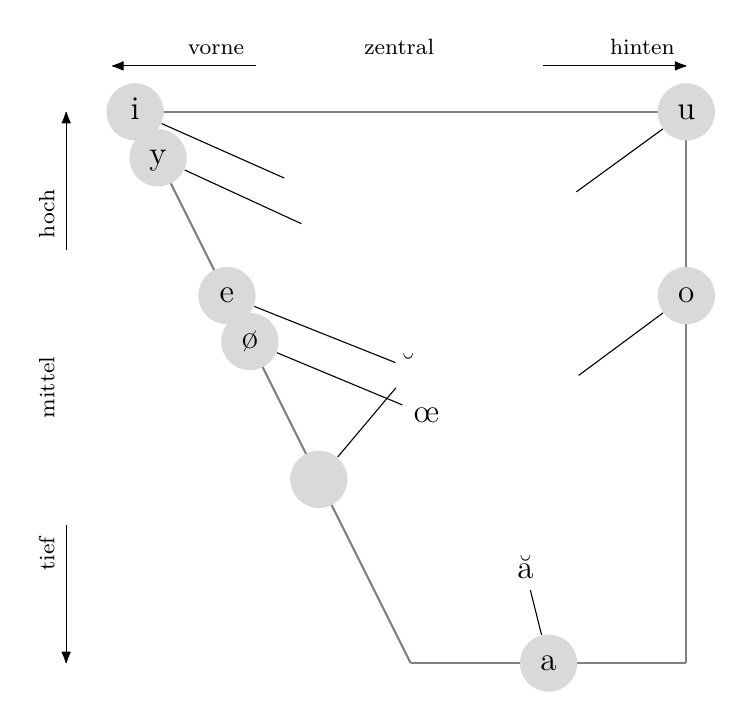
\begin{tikzpicture}[scale=3.5,baseline=default]
    \large
    \tikzset{
    vowel/.style={fill=white, anchor=mid, text depth=0ex, text height=1ex},
    vowelgespannt/.style={circle,fill=gray!30, anchor=mid, text depth=0ex, text height=1ex,minimum size=4ex},
    dot/.style={circle,fill=black,minimum size=0.4ex,inner sep=0pt,outer sep=-1pt},
    }

    \coordinate (hf) at (0,2); % high front
    \coordinate (hb) at (2,2); % high back
    \coordinate (lf) at (1,0); % low front
    \coordinate (lb) at (2,0); % low back
    \def\V(#1,#2){barycentric cs:hf={(3-#1)*(2-#2)},hb={(3-#1)*#2},lf={#1*(2-#2)},lb={#1*#2}}

    % Chart key (vorne -- hinten).
    \draw [{Latex[round]}-] (\V (-.25,0)) -- (\V (-.25,.5))  node [above left] {\footnotesize vorne};
    \draw [-{Latex[round]}] (\V (-.25,1.5)) -- (\V (-.25,2)) node [above left] {\footnotesize hinten};
    \path (\V (-.25,1)) node[above] {\footnotesize zentral};

    % Chart key (hoch--tief).
    \draw [{Latex[round]}-] (\V (0,-.25)) -- +(270:.5cm)  node [above right,rotate=90] (vokaltrapez1) {\footnotesize hoch};
    \draw [{Latex[round]}-] (\V (3,-2.5)) -- +(270:-.5cm) node [above left,rotate=90] (vokaltrapez2) {\footnotesize tief};
    \path (\V (1.5,-1)) node[above,rotate=90] {\footnotesize mittel};

    % Grid.
    \draw [gray,thick] (\V(0,0)) -- (\V(0,2));
    \draw [gray,thick] (\V(3,0)) -- (\V(3,2));
    \draw [gray,thick] (\V(0,0)) -- (\V(3,0));
    \draw [gray,thick] (\V(0,2)) -- (\V(3,2));

    \path (\V(0,0))      node[vowelgespannt] (i)   {i};
    \path (\V(0.25,0))   node[vowelgespannt] (y)   {y};
    \path (\V(0.4,0.5))  node[vowel]         (ii)  {ɪ};
    \path (\V(0.65,0.5)) node[vowel]         (yy)  {ʏ};
    \path (\V(1,0))      node[vowelgespannt] (e)   {e};
    \path (\V(1.25,0))   node[vowelgespannt] (oe)  {ø};
    \path (\V(2,0))      node[vowelgespannt] (ee)  {ɛ};
    \path (\V(1.4,0.7))  node[vowel]         (eee) {ɛ̆};
    \path (\V(1.65,0.7)) node[vowel]         (oee) {œ};
    \path (\V(3,1))      node[vowelgespannt] (a)   {a};
    \path (\V(2.5,1))    node[vowel]         (aa)  {ă};
    \path (\V (1,2))     node[vowelgespannt] (o)   {o};
    \path (\V (1.5,1.4)) node[vowel]         (oo)  {ɔ};
    \path (\V (0,2))     node[vowelgespannt] (u)   {u};
    \path (\V (0.5,1.5)) node[vowel]         (uu)  {ʊ};

    \draw (i)  -- (ii);
    \draw (y)  -- (yy);
    \draw (e)  -- (eee);
    \draw (oe) -- (oee);
    \draw (ee) -- (eee);
    \draw (a)  -- (aa);
    \draw (o)  -- (oo);
    \draw (u)  -- (uu);
  \end{tikzpicture}
  \caption[Phonologisches Vokaltrapez]{Phonologisches Vokaltrapez (Grau für [\textsc{Gespannt}: $+$])}
  \label{fig:gespanntheitbetonungundlaenge019}
  \index{Vokaltrapez}
\end{figure}

Die Vokale in den ersten Silben von \textit{Liebe} \textipa{[li:b@]}, \textit{Tüte} \textipa{[ty:t@]}, \textit{Wut} \textipa{[vu:t]}, \textit{Weg} \textipa{[ve:k]}, \textit{schön} \textipa{[S\o:n]}, \textit{Käse} \textipa{[kE:z@]}, \textit{rot} \textipa{[Ko:t]}, \textit{rate} \textipa{[Ka:t@]} gelten also gemäß dieser leicht veränderten Merkmalsmenge als \textit{gespannt}.
In diesen Beispielen sind sie betont und daher lang.
Ungespannte Vokale können betont werden, aber sie werden dadurch nicht lang, \zB \textit{Rinder} \textipa{[KInd5]}.
Formen wie *\textipa{[KI:nd5]} sind ausgeschlossen.
Tabelle~\ref{tab:gespanntheitbetonungundlaenge020} gibt einen systematischen Überblick in Form von Beispielen.

\begin{table}[!htbp]
  \centering
  \begin{tabular}{cllp{0.25cm}cll}
    \lsptoprule
    \textbf{gespannt} & \textbf{Beispiel} & \textbf{IPA} & & \textbf{ungespannt} & \textbf{Beispiel} & \textbf{IPA} \\
    \midrule
    \textipa{i}  & \textit{bieten} & \textipa{bi:t@n} && \textipa{I} & \textit{bitten}  & \textipa{bIt@n}   \\
    \textipa{y}  & \textit{fühlt}  & \textipa{fy:lt}  && \textipa{Y} & \textit{füllt}   & \textipa{fYlt}    \\
    \textipa{u}  & \textit{Mus}    & \textipa{mu:s}   && \textipa{U} & \textit{muss}    & \textipa{mUs}     \\
    \textipa{e}  & \textit{Kehle}  & \textipa{ke:l@}  && \textipa{E} & \textit{Kelle}   & \textipa{kEl@}    \\
    \textipa{E}  & \textit{stähle} & \textipa{StE:l@} && \textipa{E} & \textit{Ställe}  & \textipa{StEl@}   \\
    \textipa{\o} & \textit{Höhle}  & \textipa{h\o:l@} && \textipa{\oe} & \textit{Hölle} & \textipa{h\oe l@} \\
    \textipa{o}  & \textit{Ofen}   & \textipa{Po:f@n} && \textipa{O} & \textit{offen}   & \textipa{POf@n}   \\
    \textipa{a}  & \textit{Wahn}   & \textipa{va:n}   && \textipa{a} & \textit{wann}    & \textipa{van}     \\
    \lspbottomrule
  \end{tabular}
  \caption{Gespannte und ungespannte Vokale im Kernwortschatz}
  \label{tab:gespanntheitbetonungundlaenge020}
\end{table}

Was Gespanntheit phonetisch auszeichnet, ist nicht einfach zu bestimmen.
Man kann versuchen, die Kategorie der Gespanntheit mit einer erhöhten Muskelanspannung oder einer Veränderung der Position der Zungenwurzel in Verbindung zu bringen.
Aus Sicht der Phonologie ist der \textit{systematische} Aspekt aber wichtiger als der artikulatorische.
Für die gespannten Vokale gelten gemeinsame Strukturbedingungen, und daher sollte sie die Grammatik idealerweise als eine Klasse von Segmenten auf"|fassen -- genauso wie die stimmhaften und stimmlosen Obstruenten usw.
Mit den Ortsmerkmalen der Vokale und der Lippenrundung alleine könnte man die gespannten (und damit längbaren) Vokale aber nicht von den ungespannten unterscheiden.
Klassen definieren wir über Merkmale und Werte (vgl.\ Abschnitt~\ref{sec:merkmaleundwerte}), und daher ist das neue Merkmal gerechtfertigt.

Weil die halbvorderen und halbhinteren Vokale jetzt durch die Gespanntheit von den vorderen und hinteren unterscheidbar werden, kann ein weiteres Merkmal in seinen möglichen Werten reduziert werden.

\begin{exe}
  \ex \textsc{Lage}: \textit{vorne}, \textit{zentral}, \textit{hinten}
\end{exe}

Je nach Auf"|fassung, was der Kernwortschatz ist, gilt im Kernwortschatz (auf jeden Fall aber im Erbwortschatz), dass gespannte Vokale immer betont und damit immer lang sind.%
\footnote{Zum Kernwortschatz und Erbwortschatz s.\ Abschnitt~\ref{sec:kernundperipherie}.}
Innerhalb des Kernwortschatzes gibt es damit die in Abbildung~\ref{fig:gespanntheitbetonungundlaenge019} durch Striche verbundenen Paare aus langen gespannten betonten und kurzen ungespannten betonten oder unbetonten Vokalen.
Während die ungespannten betont oder unbetont auftreten können, sind die gespannten immer betont, vgl.\ Satz~\ref{satz:gespanntheitkern}.

\Stretch

\Satz{Gespanntheit im Kernwortschatz}{\label{satz:gespanntheitkern}%
Im Kernwortschatz sind gespannte Vokale immer betont und lang.
Zu jedem gespannten Vokal gibt es einen entsprechenden ungespannten Vokal.
Der ungespannte ist betont oder unbetont, aber immer kurz.}

Im erweiterten Wortschatz, der mehr Wörter mit drei und mehr Silben enthält, gilt die eingangs erwähnte Strukturbedingung, dass bei den gespannten Vokalen die Betonung die Länge kontrolliert.
Beispiele für unbetonte gespannte und damit kurze Vokale sind \textipa{[i]} in (\ref{ex:gespanntheitbetonungundlaenge022}), \textipa{[e]} in (\ref{ex:gespanntheitbetonungundlaenge023}), \textipa{[u]} in (\ref{ex:gespanntheitbetonungundlaenge024}), \textipa{[o]} in (\ref{ex:gespanntheitbetonungundlaenge025}), \textipa{[\o]} in (\ref{ex:gespanntheitbetonungundlaenge026}) und \textipa{[y]} in (\ref{ex:gespanntheitbetonungundlaenge027}).

\begin{exe}
  \ex\label{ex:gespanntheitbetonungundlaenge021}
  \begin{xlist}
    \ex{\label{ex:gespanntheitbetonungundlaenge022} \textit{Idee} \textipa{[Pide:]}\\
      \textit{Initiative} \textipa{[Pini\t{ts}Jati:v@]}\\
      \textit{inspirieren} \textipa{[PInspiKi:K@n]} }
    \ex{\label{ex:gespanntheitbetonungundlaenge023} \textit{Methyl} \textipa{[mety:l]}\\
      \textit{Québec} \textipa{[kebEk]}\\
      \textit{integriert} \textipa{[PIntegK\t{i5}t]}\\
      \textit{debattieren} \textipa{[debati:K@n]} }
    \ex{\label{ex:gespanntheitbetonungundlaenge024} \textit{Utopie} \textipa{[Putopi:]}\\
      \textit{Uran} \textipa{[PuKa:n]} }
    \ex{\label{ex:gespanntheitbetonungundlaenge025} \textit{Motiv} \textipa{[moti:f]}\\
      \textit{politisch} \textipa{[poli:tIS]}\\
      \textit{Phonologie} \textipa{[fonologi:]} }
    \ex{\label{ex:gespanntheitbetonungundlaenge026} \textit{Ökonomie} \textipa{[P\o konomi:]}\\
      \textit{manövrieren} \textipa{[man\o vKi:K@n]} }
    \ex{\label{ex:gespanntheitbetonungundlaenge027} \textit{Büro} \textipa{[byKo:]}\\
    \textit{Cuvée} \textipa{[kyve:]} }
  \end{xlist}
\end{exe}

Weil Wörter mit solchen Vokalen im alltäglichen Gebrauch durchaus häufig vorkommen, wird in Satz~\ref{satz:gespannterweitert} nicht von \textit{peripherem Wortschatz}, sondern vorsichtiger vom \textit{erweiterten Wortschatz} gesprochen.

\Satz{Gespanntheit im erweiterten Wortschatz}{\label{satz:gespannterweitert}%
Im erweiterten Wortschatz sind gespannte Vokale lang, wenn sie betont sind und kurz, wenn sie unbetont sind.
Auch im erweiterten Wortschatz gibt es keine ungespannten langen Vokale.
}

Völlig außerhalb dieses Systems stehen Schwa und \textipa{[5]} gemäß Satz~\ref{satz:schwabetont}.

\Satz{Schwa}{\label{satz:schwabetont}%
Schwa und \textipa{[5]} sind immer kurz und nie betont.
}

Damit müssen die zugrundeliegenden Formen genau wie bei der Endrand"=Desonorisierung gemäß der neu eingeführten Strukturbedingungen angepasst werden.
Länge muss nicht mehr zugrundeliegend spezifiziert werden, und man erhält Beispiele wie in (\ref{ex:gespanntheitbetonungundlaenge028}).

\begin{exe}
  \ex\label{ex:gespanntheitbetonungundlaenge028} \begin{xlist}
    \ex /\textipa{veg}/ \phopro \textipa{[ve:k]}
    \ex /\textipa{h\o l@}/ \phopro \textipa{[h\o:l@]}
    \ex /\textipa{of@n}/ \phopro \textipa{[Po:f@n]}
  \end{xlist}
\end{exe}

\subsection{Verteilung von [ç] und [χ]}
\label{sec:verteilungvonund}

Die sogenannten \textit{ich}- und \textit{ach}-Segmente sind komplementär verteilt.
Es gibt kein Wort, in dem sie einen lexikalischen Unterschied markieren.
Einige Beispielwörter, in denen \textipa{[\c{c}]} und \textipa{[X]} vorkommen, illustrieren dies in (\ref{ex:verteilungvonund029}).

\begin{exe}
  \ex\label{ex:verteilungvonund029}
  \begin{xlist}
    \ex{\label{ex:verteilungvonund030} krieche, schlich, Bücher, Küche, Recht, Köche}
    \ex{\label{ex:verteilungvonund031} Tuch, Geruch, hoch, Koch, Schmach, Bach}
  \end{xlist}
\end{exe}

Ausschlaggebend für das Vorkommen von \textipa{[\c{c}]} und \textipa{[X]} ist der unmittelbar vorangehende Kontext.
Nach /\textipa{i}/, /\textipa{I}/, /\textipa{y}/, /\textipa{Y}/, /\textipa{e}/, /\textipa{E}/, /\textipa{\u{E}}/, /\textipa{\o}/, /\textipa{\oe}/ kommt \textipa{[\c{c}]} vor, nach /\textipa{u}/, /\textipa{U}/, /\textipa{o}/, /\textipa{O}/, /a/ und /\textipa{\u{a}}/ hingegen \textipa{[X]}.
Nach Schwa kommt keins der beiden Segmente vor.
Ein Blick auf das phonologische Vokaltrapez in Abbildung~\ref{fig:gespanntheitbetonungundlaenge019} zeigt sofort, was der relevante Merkmalsunterschied zwischen den beiden Gruppen von Vokalen ist.
Nach Vokalen, die [\textsc{Lage}: \textit{vorne}] sind, steht \textipa{[\c{c}]}.
Nach allen anderen Vokalen steht hingegen \textipa{[X]}.
Es handelt sich hier um eine Angleichung des Artikulationsorts des Frikativs an den hinterer Vokale, eine sogenannte \textit{Assimilation}.\index{Assimilation}

Es muss jetzt nur noch entschieden werden, wie die zugrundeliegende Form in diesem Fall aussieht.
Aufschlussreich ist hier die Betrachtung von Wörtern wie \textit{Milch} /\textipa{mIl\c{c}}/, \textit{Storch} /\textipa{StOK\c{c}}/ oder \textit{Röckchen} /\textipa{K\oe k\c{c}@n}/, in denen \textipa{[\c{c}]}, aber niemals \textipa{[X]} nach einem Konsonanten vorkommt.
Dies ist generell der Fall, und es ist deswegen günstiger, anzunehmen, dass /\textipa{\c{c}}/ zugrundeliegt und \textipa{[X]} das phonetische Resultat einer Assimilation ist.
Das heißt, dass \textipa{[X]} kein zugrundeliegendes Segment ist und nicht in /~/ gehört.
Mit der entsprechenden Strukturbedingung aus Satz~\ref{satz:cassimilation} ergeben sich die Beispiele wie in (\ref{ex:verteilungvonund032}).

\Satz{/ç/-Assimilation}{\label{satz:cassimilation}%
[ç] kann nicht nach Vokalen stehen, die nicht [\textsc{Lage}: \textit{vorne}] sind.
Zugrundeliegendes /\textipa{\c{c}}/ wird daher nach zentralen und hinteren Vokalen weiter hinten artikuliert, nämlich als \textipa{[X]}.}

\begin{exe}
  \ex\label{ex:verteilungvonund032}
  \begin{xlist}
    \ex{/\textipa{I\c{c}}/ \phopro \textipa{[PI\c{c}]}}
    \ex{/\textipa{\u{a}\c{c}}/ \phopro \textipa{[PaX]}}
  \end{xlist}
\end{exe}

\subsection{/ʁ/-Vokalisierungen}
\label{sec:vokalisierungen}

In Abschnitt~\ref{sec:orthographischesr} wurden phonetische Korrelate von geschriebenem \textit{r} besprochen.
Die Schrift ist hier besonders systematisch, denn orthographisches \textit{r} entspricht immer einem zugrundeliegenden /\textipa{K}/ (s.\ auch Abschnitt~\ref{sec:buchstabenundphonologischesegmente}).
In (\ref{ex:vokalisierungen033}) sind Beispiele zusammengestellt (inklusive der Silbengrenzen), die dies illustrieren.

\begin{exe}
  \ex\label{ex:vokalisierungen033}
  \begin{xlist}
    \ex{kleiner \textipa{[kl\t{aE}.n5]}, kleinere \textipa{[kl\t{aE}.n@.K@]}}
    \ex{Bär \textipa{[b\t{E5}]}, Bären \textipa{[bE:.K@n]}}
    \ex{knarr \textipa{[kn\t{a@}]}, knarre \textipa{[kna.K@]}}
  \end{xlist}
\end{exe}

Wenn ein zugrundeliegendes /\textipa{K}/ am Silbenanfang steht, wird es als Konsonant \textipa{[K]} realisiert.
Demgegenüber findet am Silbenende immer eine Vokalisierung von /\textipa{K}/ statt.
Nach gespannten Vokalen wird /\textipa{K}/ zu \textipa{[5]}, nach ungespannten zu \textipa{[@]}.
Nach (stets unbetontem) Schwa wird /\textipa{K}/ gar nicht realisiert, und Schwa wird zu \textipa{[5]}.
Diese Vorgänge formal genau aufzuschreiben, würde den hier gegebenen Rahmen sprengen.
Aus Sicht der Phonologie sind die Unterschiede zwischen \textipa{[@]} und \textipa{[5]} auch nicht erheblich, denn diese Segmente stellen nur minimal unterschiedliche Färbungen des Schwa-Segments dar.
Beispiele folgen in (\ref{ex:vokalisierungen034}).

\begin{exe}
  \ex \label{ex:vokalisierungen034}
  \begin{xlist}
    \ex /\textipa{kl\t{aE}n@K}/ \phopro \textipa{[kl\t{aE}.n5]}
    \ex /\textipa{tiK}/ \phopro \textipa{[t\t{i5}]}
    \ex /\textipa{bIKk@}/ \phopro \textipa{[b\t{I@}.k@]}
  \end{xlist}
\end{exe}

Die entsprechende Strukturbedingung und ihre Effekte werden in Satz~\ref{satz:rvokalisierung} beschrieben.

\Satz{/ʁ/-Vokalisierung}{\label{satz:rvokalisierung}%
Zugrundeliegendes /\textipa{K}/ kann nicht am Silbenende stehen.
Es wird in dieser Position als Schwa-Segment im sekundären Diphthong realisiert.
Nach gespanntem Vokal folgt \textipa{[5]}, nach ungespanntem folgt \textipa{[@]}.
Schwa und /\textipa{K}/ werden zusammen durch \textipa{[5]} substituiert.
}

\Zusammenfassung{%
In der Phonologie ist der Status der Segmente im Gesamtsystem relevant.
Dabei werden vor allem ihre Verteilung und ihre Merkmale betrachtet.
Wenn man alle Formen eines Worts berücksichtigt, kann man umgebungsabhängige bzw.\ positionsabhängige Änderungen von Merkmalswerten beobachten.
Um solche Phänomene adäquat zu beschreiben, nimmt man abstraktere zugrundeliegende Formen an, die an phonologische Strukturbedingungen wie die Endrand-Desonorisierung angepasst werden.
}

\section{Silben und Wörter}
\label{sec:silbenundwoerter}

\subsection{Phonotaktik}
\label{sec:phonotaktik}

Aufbauend auf der Beschreibung der einzelnen Segmente kann und sollte außerdem angegeben werden, wie diese Segmente zu größeren Einheiten zusammengesetzt werden, wie also die \textit{phonologische Struktur} aufgebaut wird (zum Strukturbegriff vgl.\ Abschnitt~\ref{sec:strukturbildung}).
Die Wörter in (\ref{ex:phonotaktik035}) sind Phantasiewörter in Pseudo-Standardorthographie und hypothetischer phonetischer Umschrift.

\begin{exe}
  \ex\label{ex:phonotaktik035}
  \begin{xlist}
    \ex{\label{ex:phonotaktik036} Nka \textipa{[Nka:]}, Totk \textipa{[tOtk]}, Pkafkme \textipa{[pkafkm@]}}
    \ex{\label{ex:phonotaktik037} Klie \textipa{[kli:]}, Filb \textipa{[fIlp]}, Ronge \textipa{[KON@]}}
  \end{xlist}
\end{exe}

Die hypothetischen Wörter in (\ref{ex:phonotaktik036}) unterscheiden sich deutlich von denen in (\ref{ex:phonotaktik037}).
Während die zweite Gruppe nämlich zumindest \textit{mögliche} Wörter des Deutschen enthält, enthält die erste Gruppe nur Wörter, die aus irgendeinem Grund auf keinen Fall Wörter des Deutschen sein könnten.
Der Grund dafür ist, dass die erste Gruppe \textit{phonotaktisch nicht wohlgeformte Wörter bzw.\ Silben} enthält.
Es muss also Regularitäten geben, nach denen sich Segmente des Deutschen zu größeren Einheiten wie Silben und Wörtern zusammensetzen.
Diese Regularitäten beschreibt gemäß Definition~\ref{def:phonotaktik} die \textit{Phonotaktik}.

\Definition{Phonotaktik}{\label{def:phonotaktik}%
Die \textit{Phonotaktik} beschreibt die Regularitäten, nach denen Segmente zu größeren Strukturen zusammengesetzt werden.
Die Phonotaktik definiert dabei Einheiten wie die Silbe und das Wort.
\index{Phonotaktik}
}

Die Silbe ist die Einheit, mittels derer alle wesentlichen Einschränkungen für mögliche Segmentfolgen formuliert werden können.
Dieser Abschnitt ist daher ausschließlich der Silbe gewidmet.

\subsection{Silben}
\label{sec:silben}

\index{Silbe}

Präzise zu definieren, was eine Silbe ist, ist keine triviale Aufgabe.
Intuitiv sind sie Einheiten, die größer sein können (aber nicht müssen) als Segmente, aber kleiner sein können (nicht müssen) als Wörter.
Der damit theoretisch mögliche Extremfall, bei dem Segment, Silbe und Wort zusammenfallen, tritt im Deutschen nicht auf, weil im Wortanlaut immer ein Konsonant steht, ggf.\ der Glottalplosiv.
Selbst in marginalen \textit{Interjektionen} (\textit{Rufwörtern}) wie \textit{oh} \textipa{[Po:]} und \textit{ah} \textipa{[Pa:]} besteht die Silbe (und damit das Wort) aus einem Konsonanten und einem Vokal.
Wenn man Diphthonge als ein Segment zählt, ist das Substantiv \textit{Ei} \textipa{[P\t{aE}]} ähnlich.
In anderen Sprachen, die den obligatorisch konsonantischen Wortanlaut nicht haben, ist der Maximalfall (Zusammenfall von Segment, Silbe und Wort) auch eher selten.
Die französischen Substantive \textit{œufs} \textipa{[\o:]} `Eier' (nur im Plural) oder \textit{eau} \textipa{[o:]} `Wasser' sowie das schwedische Substantiv \textit{ö} \textipa{[\oe:]} `Insel' (nur im Singular) stellen auch innerhalb ihrer eigenen Sprachsysteme eher Exoten dar.
In deutschen Wörter wie \textit{Ehe} \textipa{[Pe:@]} fallen in der zweiten Silbe zumindest aber Segment und Silbe \textipa{[@]} zusammen.

Im Normalfall bestehen Silben aus mehreren Segmenten, und Wörter bestehen häufig aus mehreren Silben.
Beispiele für einsilbige Wörter aus zwei Segmenten im Deutschen sind \textit{Schuh} \textipa{[Su:]} oder \textit{Tee} \textipa{[te:]}, Beispiele für zweisilbige Wörter aus zweisegmentalen Silben sind \textit{Tüte} \textipa{[ty:t@]} oder \textit{rege} \textipa{[Ke:g@]}.
Ein einsilbiges Wort mit deutlich mehr als zwei Segmenten ist \textit{Strauch} \textipa{[StK\t{aO}X]}.
Eine wesentliche Frage der Silbenphonologie ist, wie hoch die Komplexität solcher Strukturen maximal ist.

\index{Silbe!Klatschmethode}

In der Grundschuldidaktik wird oft über die \textit{Klatschmethode} versucht, Kindern ein Gefühl für Silben zu vermitteln.
Dabei wird gesagt, dass jedes Stück eines Wortes, zu dem man bei abgehacktem Sprechen einmal klatschen kann, eine Silbe sei.
Diese Methode ist zuerst einmal deshalb problematisch, weil sie nur mit einer unnatürlichen oder sogar falschen Aussprache funktioniert.
Es bei normaler Aussprache im Deutschen viel natürlicher, auf Wörter wie \textit{Ratte} \textipa{[Kat@]} nur einmal zu klatschen.
Konkret handelt es sich beim Wort \textit{Ratte} um einen Trochäus (siehe Abschnitt~\ref{sec:wortakzentimdeutschen}) mit einem Silbengelenk (siehe Abschnitt~\ref{sec:einsilblerundzweisilbler}).
Beim Sprechen wird hier der Druck in einem Zug über beide Silben abgelassen, anders als bei Wörtern wie \textit{Rate}.%
\footnote{Wie \citet[15--16]{Maas2002} zeigt, sind die Grundlagen für dieses Analyse bereits von \citet{Sievers1876} gelegt worden.}
Abgesehen davon geht es bei der Anwendung der Methode meist um das Vermitteln der orthographisch korrekten Silbentrennnung.
Die Beherrschung der entsprechenden Regeln erfordert aber subtilere Kenntnisse grammatischer Regularitäten, als sie die Klatschmethode vermitteln kann.
Ein Kind wird durch das Klatschen vielleicht mit etwas Glück lernen, dass Wörter wie \textit{Kriecher}, \textit{Iglu} oder \textit{Ratte} aus genau zwei Silben bestehen.
Ob die Silbentrennung aber \textit{Krie-cher} oder \textit{Kriech-er}, \textit{I-glu} oder \textit{Ig-lu} und \textit{Ratt-e}, \textit{Rat-te} oder \textit{Ra-tte} ist, ist durch Klatschen nicht erlernbar.
Bei diesen Wörtern handelt es sich nicht um Sonderfälle, sondern sie stehen für systematische Probleme der Klatschmethode.
Wegen dieser grundlegenden Probleme müssen Lehrpersonen bei Klatsch-Übungen wie oben bereits angedeutet unnatürliche Aussprachen vormachen, \zB \textipa{[Kat]} -- \textipa{[te:]}.
Gerade dieses Abhacken macht \textit{Kriech-er} aber genauso plausibel wie \textit{Krie-cher}.
Um die zerhackte Aussprache in Fällen mit orthographischen Doppelkonsonanten wie \textipa{[Kat]} -- \textipa{[te:]} überhaupt artikulieren zu können, muss man zudem paradoxerweise bereits Kenntnisse der Orthographie und Silbentrennung besitzen.
Man dreht sich also im Kreis, und ein solider Lernerfolg durch das Klatschen ist nicht zu erwarten.

Trotz ihrer absoluten Unzulänglichkeit für den Grundschulunterricht veranschaulicht die Klatschmethode allerdings ein wichtiges Prinzip der Silbenbildung.
Silben bringen die Segmente in eine rhythmische Ordnung, die charakteristischen artikulatorischen Einheiten entspricht.
Diese artikulatorischen Einheiten sind Schübe, die im Prinzip einem Öffnen und Schließen des Vokaltrakts entsprechen.
An einsilbigen Wörtern wie \textit{Tag} \textipa{[ta:k]} oder \textit{gut} \textipa{[gu:t]} sieht man, dass sie mit einem Verschluss beginnen und mit einem Verschluss enden, während in der Mitte beim Vokal der Vokaltrakt geöffnet ist (genauer in Abschnitt~\ref{sec:sonoritaet}).
Im Kern der Silbe befindet sich passend dazu im Deutschen immer ein Vokal, also ein Segment, bei dem sich die Artikulatoren gar nicht punktuell annähern (Abschnitt~\ref{sec:vokale}).
Die Klatschmethode kann man also auf die Anweisung reduzieren, bei jedem Vokal einmal zu klatschen, und mehr gibt sie prinzipiell nicht her.
Wie an den Zweifelsfällen weiter oben gezeigt wurde, löst das aber nicht das Problem, ob Konsonanten zwischen den Vokalen in mehrsilbigen Wörtern zur ersten oder zweiten Silbe gehören.

Schwieriger wird die Silbenphonologie dadurch, dass in den verschiedenen Formen eines Wortes die Silbengrenzen nicht immer konstant sind.\index{Silbe!Grenze}
Anders gesagt ist die Silbenstruktur von Wörtern nicht im Lexikon festgelegt.
Die Beispiele (\ref{ex:silben038}) zeigen dies.
In der Transkription werden die Silbengrenzen durch einen einfachen Punkt markiert.

\begin{exe}
  \ex\label{ex:silben038}
  \begin{xlist}
    \ex{Ball \textipa{[bal]}, Bälle \textipa{[bE.l@]}, Balls \textipa{[bals]}}
    \ex{Sturm \textipa{[St\t{U@}m]}, Stürme \textipa{[St\t{Y@}.m@]}}
    \ex{Mittelstürmer \textipa{[mI.t@l.St\t{Y@}.m5]}, Mittelstürmerin \textipa{[mI.t@l.St\t{Y@}.m@.KIn]}}
  \end{xlist}
\end{exe}

Ein Wort wie \textit{Ball} ist im Nominativ Singular einsilbig, und das \textipa{[l]} steht im Auslaut (am Ende) dieser einen Silbe.
Mit dem hinzutretenden \textipa{[@]} der Plural-Endung verändert sich auch die Silbenstruktur:
Das \textipa{[l]} steht im Anlaut (am Anfang) der zweiten Silbe.
Ähnliches passiert bei \textit{Sturm} und \textit{Stürme} mit dem \textipa{[m]}.
Bei \textit{Mittelstürmer} \textipa{[mI.t@l.St\t{Y@}.m5]} und \textit{Mittelstürmerin} \textipa{[mI.t@l.St\t{Y@}.m@.KIn]} wird die Beschreibung noch schwieriger, weil /\textipa{K}/ nur dann als Konsonant \textipa{[K]} realisiert wird, wenn noch ein Vokal in derselben Silbe folgt, wenn also das /\textipa{K}/ im Silbenanlaut steht (vgl.\ dazu genauer Abschnitt~\ref{sec:vokalisierungen}).
Wenn wie in \textit{Balls} aber ein \textipa{[s]} hinzutritt, bleibt das Wort einsilbig, und das \textipa{[s]} wird an die einzige Silbe hinten angehängt.
Die Silbenbildung kann also kein phonetisches, sondern sie muss ein phonologisches Phänomen sein.
Ihre Beschreibung erfordert es, dass das Gesamtsystem (also \zB alle Formen eines Wortes) betrachtet wird.
Entsprechend wird Definition~\ref{def:silbe} gegeben.

\Definition{Silbe und Silbifizierung}{\label{def:silbe}%
\textit{Silben} sind die nächstgrößeren phonologischen Einheiten nach den Segmenten.
Die Segmente sind ihre kleinsten Konstituenten.
Die Silbenstruktur ist nicht im Lexikon abgelegt und wird durch den phonologischen Prozess der \textit{Silbifizierung} zugewiesen.
\index{Silbe}
}

Mit Klatschen ist es also nicht getan.
Der analytische Einstieg in die Silbenstruktur des Deutschen gelingt am leichtesten über einsilbige Wörter.
Die Abschnitte~\ref{sec:deranfangsrandimeinsilbler} und~\ref{sec:derendrandimeinsilbler} leisten (nach der Einführung einiger technischer Begriffe in Abschnitt~\ref{sec:silbenstruktur}) daher zunächst eine einfache Beschreibung möglicher einsilbiger Wörter des Deutschen.
Die Verallgemeinerung zu mehrsilbigen Wörtern erfolgt nach einer theoretischen Ergänzung (Abschnitte~\ref{sec:sonoritaet} und~\ref{sec:diesystematikderraender}) in Abschnitt~\ref{sec:einsilblerundzweisilbler}.

\subsection{Silbenstruktur}
\label{sec:silbenstruktur}

\begin{figure}[!htbp]
  \centering
  \begin{forest}
    [Silbe, calign=last
      [Anfangsrand, sake, calign=first
        [C][C]
      ]
      [Reim
        [Kern, sake,calign=first
          [V]
        ]
        [Endrand, sake, calign=last
          [C][C]
        ]
      ]
    ]
  \end{forest}
  \caption{Allgemeines Schema für die Silbenstruktur von Silben mit zwei Konsonanten im Anfangsrand und im Endrand}
  \label{fig:silbenstruktur039}
\end{figure}

In diesem Abschnitt wird die Terminologie eingeführt, mit der man über Positionen in der Silbe redet.
Offensichtlich bilden Silben komplexere Strukturen aus, die sich um einen Vokal oder Diphthong im \textit{Kern} herum gruppieren.%
\footnote{Eine alternative Sichtweise würde bei Diphthongen das zweite Glied nicht als Teil des Kerns, sondern des Endrands (s.\,u.) analysieren.
Für unsere Zwecke ist der sich ergebende theoretische Unterschied vernachlässigbar.}
Für die drei sich ergebenden Konstituenten der Silbe gibt es verschiedene Bezeichnungen, von denen hier \textit{Anfangsrand}, \textit{Kern} und \textit{Endrand} verwendet werden.
Aus Gründen, die erst in Abschnitt~\ref{sec:einsilblerundzweisilbler} diskutiert werden, hat es sich als nützlich erwiesen, Kern und Endrand zu einer eigenen Konstituente, dem \textit{Reim} zusammenzufassen.\index{Silbe!Reim}
Neben Definition~\ref{def:silbenstruktur} wird eine Baumdarstellung der allgemeinen Silbenstruktur für Silben mit je zwei Konsonanten im Anfangsrand und im Endrand in Abbildung~\ref{fig:silbenstruktur039} und ein passendes Beispiel (\textit{fremd}) in Abbildung~\ref{fig:silbenstruktur040} gegeben.
Es werden C und V als Abkürzungen für \textit{Konsonant} und \textit{Vokal} verwendet und im Anfangs- und Endrand je zwei Konsonantenpositionen angenommen.
In Abschnitt~\ref{sec:diesystematikderraender} wird argumentiert, dass dies tatsächlich die maximale Komplexität der Ränder ist.

\Definition{Einheiten der Silbenstruktur}{\label{def:silbenstruktur}%
Der \textit{Silbenkern} (der \textit{Nukleus}) wird typischerweise durch einen Vokal oder Diphthong gebildet.
(Manche Konsonanten wie Nasale und Liquide können atypisch im Kern stehen.)
Vor und nach dem Kern können Konsonanten stehen, die den \textit{Anfangsrand} (den \textit{Onset}) bzw.\ den \textit{Endrand} (die \textit{Coda}) bilden.
Es gibt keine Silben mit leerem Kern.
Kern und Endrand bilden den \textit{Reim}.
\index{Silbe!Kern}
\index{Silbe!Anfangsrand}
\index{Silbe!Endrand}
\index{Silbe!Reim}
}

\begin{figure}[!htbp]
  \centering
  \begin{forest}
    [Silbe, calign=last
      [Anfangsrand, ake, calign=first
        [f][ʁ]
      ]
      [Reim, calign=first
        [Kern,ake
          [ɛ]
        ]
        [Endrand, ake, calign=last
          [m][t]
        ]
      ]
    ]
  \end{forest}
  \caption{Beispiel für Silbenstruktur (\textit{fremd})}
  \label{fig:silbenstruktur040}
\end{figure}

\subsection{Der Anfangsrand im Einsilbler}
\label{sec:deranfangsrandimeinsilbler}

In diesem und dem nächsten Abschnitt werden einsilbige Wörter herangezogen, um die minimale und die maximale Komplexität deutscher Silben zu ermitteln.
Ein einsilbiges Wort wird üblicherweise \textit{Einsilbler} genannt.\index{Einsilbler}
In Abschnitt~\ref{sec:silben} wurde bereits festgestellt, dass Silben -- und damit auch Einsilbler -- mindestens aus einem Vokal oder Diphthong im Silbenkern bestehen.
Gleichzeitig enthält eine Silbe immer genau einen (niemals zwei oder mehr) Vokale.
Diesem Vokal geht im Deutschen immer der Glottalplosiv voraus, wenn kein anderer Konsonant vorausgeht.
Maximal einfache Einsilbler sind also die in (\ref{ex:deranfangsrandimeinsilbler041}), wobei Diphthonge wie ein einfacher Vokal behandelt werden.%
\footnote{Weil die Silbifizierung nicht in den zugrundeliegenden Formen spezifiziert ist, werden silbifizierte Wörter konsequent in [~] gesetzt.}

\begin{exe}
  \ex\label{ex:deranfangsrandimeinsilbler041}
  \begin{xlist}
    \ex Ei \textipa{[P\t{aE}]}
    \ex eh \textipa{[Pe:]}
    \ex ah \textipa{[Pa:]}
    \ex oh \textipa{[Po:]}
  \end{xlist}
\end{exe}

Wir beginnen mit dem Anfangsrand und überlegen der Reihe nach, ob dort ein, zwei oder auch mehr Segmente stehen können, und falls es so ist, welche und in welcher Reihenfolge.
Der Anfangsrand kann durch ein einzelnes konsonantisches Segment einer beliebigen Artikulationsart besetzt werden.
In (\ref{ex:deranfangsrandimeinsilbler043}) sind es stimmlose und stimmhafte Plosive, in (\ref{ex:deranfangsrandimeinsilbler044}) stimmlose und stimmhafte Frikative bis auf \textipa{[\c{c}]}, in (\ref{ex:deranfangsrandimeinsilbler045}) Nasale bis auf \textipa{[N]} und in (\ref{ex:deranfangsrandimeinsilbler046}) der Approximant.
Der Nasal \textipa{[N]} sowie der Frikativ \textipa{[\c{c}]} kommen prinzipiell im Anfangsrand von Einsilblern nicht vor und werden aus allen weiteren Überlegungen über diese Position ausgeschlossen.%
\footnote{Nur die Beispielwörter, die in diesem Abschnitt unmögliche Kombinationen illustrieren sollen, werden in IPA-Transkription wiedergegeben, der Rest orthographisch.
Es ist zu beachten, dass die entsprechenden Wörter nicht einfach nur durch Zufall nicht existieren.
Sie könnten vielmehr keine Wörter des Deutschen sein, weil das System die entsprechenden Silbenstrukturen nicht zulässt.}

\Np

\begin{exe}
  \ex\label{ex:deranfangsrandimeinsilbler042}
  \begin{xlist}
    \ex{\label{ex:deranfangsrandimeinsilbler043} Kuh, geh}
    \ex{\label{ex:deranfangsrandimeinsilbler044} Schuh, hau, Reh, Vieh, wo, *\textipa{[\c{c}i:]}}
    \ex{\label{ex:deranfangsrandimeinsilbler045} nie, mäh, *\textipa{[Nu:]}}
    \ex{\label{ex:deranfangsrandimeinsilbler046} lau}
  \end{xlist}
\end{exe}

Wenn im Anfangsrand \textit{zwei} Konsonanten stehen, sind die Kombinationsmöglichkeiten bereits erheblich eingeschränkt.
In unseren Überlegungen setzen wir jetzt jeweils (in dieser Reihenfolge) Plosive, Frikative, Nasale und Approximanten als zweites Segment im Anfangsrand ein und überlegen, welche Segmente dann jeweils davor stehen können.
Die Beispiele sind möglichst so gewählt, dass rechts vom Vokal nichts steht, aber wenn ein solches Beispiel zufällig nicht existiert, wird auf andere Einsilbler ausgewichen.
Plosive an zweiter Position sind im zweisegmentalen Anfangsrand nahezu unmöglich -- vgl.\ (\ref{ex:deranfangsrandimeinsilbler048}) -- mit der Ausnahme von \textipa{[p]} und \textipa{[t]} nach \textipa{[S]} wie in (\ref{ex:deranfangsrandimeinsilbler049}).
Es gibt jedoch Lehnwörter (meist keine Einsilbler), die abweichende Konsonantenverbindungen links vom Vokal enthalten.
Diese wenigen Ausnahmen wie in (\ref{ex:deranfangsrandimeinsilbler050}) sind wegen dieses ungewöhnlichen Silbenbaus nicht zum Kern des Systems zu rechnen (s.\ Abschnitt~\ref{sec:kernundperipherie}).
Sie sind also nicht nur Lehnwörter, sondern auch Fremdwörter.
Wörter wie \textit{stygisch} sind im Übrigen nur dann betroffen, wenn \textipa{[st]} statt \textipa{[St]} gesprochen wird.

\begin{exe}
  \ex\label{ex:deranfangsrandimeinsilbler047}
  \begin{xlist}
    \ex{\label{ex:deranfangsrandimeinsilbler048} *\textipa{[pte:]}, *\textipa{[fpe:]}, *\textipa{[Sgu:]}, *\textipa{[lta:]} usw.}
    \ex{\label{ex:deranfangsrandimeinsilbler049} spei, steh}
    \ex{\label{ex:deranfangsrandimeinsilbler050} Pte(ranodon), chtho(nisch), sty(gisch)}
  \end{xlist}
\end{exe}

Da wir \textipa{[\t{pf}]} wie in \textit{Pfau} und \textipa{[\t{ts}]} wie in \textit{zieh} sowie das seltene \textipa{[\t{tS}]} wie in \textit{Chips} als Affrikaten (also jeweils nur einen Konsonanten) auf"|fassen (Abschnitt~\ref{sec:affrikaten}), treten die Frikative \textipa{[f]}, \textipa{[s]}, \textipa{[S]}, \textipa{[h]}, \textipa{[z]} und \textipa{[J]} niemals als zweites Segment im Anfangsrand auf, vgl.\ (\ref{ex:deranfangsrandimeinsilbler052}).%
\footnote{Die Kombination \textipa{[tJ]} bzw.\ \textipa{[t\c{c}]} wie in \textit{tja} oder dem norddeutschen Namen \textit{Tjark} ist überaus selten und muss nicht in die Beschreibung des Systemkerns aufgenommen werden.}
Nur \textipa{[K]} kommt vor, aber nur nach den Plosiven und \textipa{[f]}, \textipa{[S]} sowie selten \textipa{[v]} (\ref{ex:deranfangsrandimeinsilbler053}).
Außerdem findet man \textipa{[v]}, aber nur nach \textipa{[k]} und \textipa{[S]} wie in (\ref{ex:deranfangsrandimeinsilbler054}).

\begin{exe}
  \ex\label{ex:deranfangsrandimeinsilbler051}
  \begin{xlist}
    \ex{\label{ex:deranfangsrandimeinsilbler052} *\textipa{[ksi:]}, *\textipa{[tfa:]}, *\textipa{[gz\t{aO}]} usw.}
    \ex{\label{ex:deranfangsrandimeinsilbler053} Pracht, brüh, trau, dreh, kräh, grau, früh, Schrei, Wrack}
    \ex{\label{ex:deranfangsrandimeinsilbler054} Qual, Schwur}
  \end{xlist}
\end{exe}

Nasale an zweiter Position im Anfangsrand sind selten, sowohl nach Plosiven (\ref{ex:deranfangsrandimeinsilbler056}) als auch nach Frikativen (\ref{ex:deranfangsrandimeinsilbler057}).
Die einzigen systematischen Ausnahmen sind \textipa{[kn]} und selten \textipa{[gn]} (\ref{ex:deranfangsrandimeinsilbler058}) sowie \textipa{[Sn]} und \textipa{[Sm]} (\ref{ex:deranfangsrandimeinsilbler059}).%
\footnote{Wörter mit \textipa{[pn]} sind seltene Lehnwörter wie \textit{Pneu}.
Das einzige häufiger vorkommende Erbwort mit \textipa{[gn]} in einem Anfangsrand ist \textit{Gnade}.
Alle anderen Wörter (\zB dialektal gefärbte wie \textit{Gnatz} und \textit{Gnitze} oder Lehnwörter wie \textit{Gnom} oder \textit{Gnosis}) haben eine niedrige Typen- und Tokenhäufigkeit (s.\ Abschnitt~\ref{sec:kernundperipherie}).
Ob \textipa{[gn]} im Anfangsrand also zum Kern des Systems gehört, ist fraglich.}

\Np

\begin{exe}
  \ex\label{ex:deranfangsrandimeinsilbler055}
  \begin{xlist}
    \ex{\label{ex:deranfangsrandimeinsilbler056} *\textipa{[pme:]}, *\textipa{[bn\t{aO}]}, *\textipa{[tne:]} usw.}
    \ex{\label{ex:deranfangsrandimeinsilbler057} *\textipa{[fn\t{aO}]}, *\textipa{[smu:]}, *\textipa{[Kni:]} usw.}
    \ex{\label{ex:deranfangsrandimeinsilbler058} Knie, Gnade}
    \ex{\label{ex:deranfangsrandimeinsilbler059} Schnee, schmäh}
  \end{xlist}
\end{exe}

Der einzige laterale Approximant des Deutschen \textipa{[l]} an zweiter Position steht nach allen Plosiven mit Ausnahme der alveolaren (\ref{ex:deranfangsrandimeinsilbler061}).
Außerdem findet man ihn nach den stimmlosen Frikativen \textipa{[f]} und \textipa{[S]} (\ref{ex:deranfangsrandimeinsilbler062}).
Diese Verbindungen sind die typischsten Anfangsränder aus zwei Segmenten.

\begin{exe}
  \ex\label{ex:deranfangsrandimeinsilbler060}
  \begin{xlist}
    \ex{\label{ex:deranfangsrandimeinsilbler061} Plan, blüh, *\textipa{[tly:]}, *\textipa{[dly:]}, Klee, glüh}
    \ex{\label{ex:deranfangsrandimeinsilbler062} flieh, Schlag}
  \end{xlist}
\end{exe}

Die strukturellen Möglichkeiten für dreisegmentale Anfangsränder sind auf \textipa{[SpK]} und \textipa{[StK]} beschränkt (\ref{ex:deranfangsrandimeinsilbler064}).
Die wenigen (nicht einsilbigen) Wörter mit \textipa{[Spl]} im Anfangsrand (\ref{ex:deranfangsrandimeinsilbler065}) gehören wohl alle zur selben germanischen Grundform, sind dabei dialektal gefärbt bzw.\ aus dem Englischen entlehnt und können als peripher vernachlässigt werden.

\begin{exe}
  \ex\label{ex:deranfangsrandimeinsilbler063}
  \begin{xlist}
    \ex{\label{ex:deranfangsrandimeinsilbler064} sprüh, Stroh}
    \ex{\label{ex:deranfangsrandimeinsilbler065} Splitter, spleiß, Spliss}
  \end{xlist}
\end{exe}

Im komplexen Anfangsrand sind häufig (im Sinn einer Typenhäufigkeit, s.\ Abschnitt \ref{sec:kernundperipherie}) vor allem Kombinationen aus Plosiv und \textipa{[K]} oder \textipa{[l]}.
Die Präferenz für diese Kombination hat Einzelsprachen übergreifende Züge.
Man fasst daher \textit{r}- und \textit{l}-Segmente zu den sogenannten \textit{Liquiden} (oder \textit{Fließlauten}) zusammen, um ihrem ähnlichen Verhalten beim Silbenbau Rechnung zu tragen, s.\ Definition~\ref{def:liquid}.
In der weiteren Beschreibung der Silbe wird sich diese Klassenbildung sofort weiter auszahlen.
\index{Liquid}

\Definition{Liquid}{\label{def:liquid}%
\textit{Liquide} sind \textit{l}- und \textit{r}-Segmente.
Die Gruppierung erfolgt für das Deutsche auf Basis phonologischer, nicht aber artikulatorischer Kriterien.
}

\subsection{Der Endrand im Einsilbler}
\label{sec:derendrandimeinsilbler}

Der Endrand wird jetzt etwas kompakter abgearbeitet als der Anfangsrand.
Auf die Auf"|listung strukturell unmöglicher Pseudo-Beispiele wird aus Gründen der Übersichtlichkeit verzichtet.
Zusätzlich fassen wir \textipa{[l]} und \textipa{[K]} wie am Ende von Abschnitt~\ref{sec:deranfangsrandimeinsilbler} vorgeschlagen zur Gruppe der Liquide zusammen.%
\footnote{Dabei ist zusätzlich zu bedenken, dass \textipa{[K]} im Endrand phonetisch als Vokal artikuliert wird.}
Weiterhin kann man feststellen, dass im Endrand wegen der Endrand-Desonorisierung (Abschnitte~\ref{sec:endranddesonorisierung1} und~\ref{sec:endranddesonorisierung}) keine stimmhaften Obstruenten vorkommen können, und dass damit \textipa{[b d g v z J]} aus der Betrachtung ausgeschlossen werden können.
Wenn die zugrundeliegend stimmhaften Obstruenten in den Endrand geraten, verhalten sie sich wie ihre stimmlosen Pendants.
Ebenso tritt \textipa{[h]} nur im Anfangsrand auf.
Schließlich sind \textipa{[\c{c}]} und \textipa{[X]} Manifestationen eines zugrundeliegenden Segments /\textipa{\c{c}}/ und müssen daher nicht getrennt behandelt werden.

Die nicht explizit aus diesen Gründen ausgeschlossenen Segmente treten alle in simplexen Endrändern des Kernwortschatzes auf.
Beispiele für einfache Endränder werden in (\ref{ex:derendrandimeinsilbler066}) gegeben.

\begin{exe}
  \ex\label{ex:derendrandimeinsilbler066}
  \begin{xlist}
    \ex ab, Hut, Rock
    \ex auf, aus, Hasch, ich
    \ex Raum, Zaun, Fang
    \ex Ohr, voll
  \end{xlist}
\end{exe}

Bei den zweisegmentalen Endrändern verfahren wir genau wie bei den zweisegmentalen Anfangsrändern.
Wir gehen also die Segmente der verschiedenen Artikulationsarten (Plosive, Frikative, Nasale, Liquide) an erster Position im Endrand -- sozusagen von innen nach außen -- durch und prüfen, inwiefern sie die Wahl des zweiten Segments einschränken.
Anders als im Anfangsrand sind zunächst Folgen aus zwei Plosiven zulässig, allerdings von allen sechs theoretischen Möglichkeiten nur \textipa{[pt]} und \textipa{[kt]}.%
\footnote{Da wegen der Endrand-Desonorisierung nur \textipa{[k]}, \textipa{[t]} und \textipa{[p]} betrachtet werden müssen, sind die theoretisch möglichen Kombinationen jeweils eins dieser drei Segmente gefolgt von einem der anderen beiden, also \textipa{[kt]}, *\textipa{[kp]}, *\textipa{[tk]}, *\textipa{[tp]}, *\textipa{[pk]} und \textipa{[pt]}.}

\begin{exe}
  \ex\label{ex:derendrandimeinsilbler067}
  \begin{xlist}
    \ex Abt, schleppt, klappt
    \ex Takt, Sekt, nackt, rückt
  \end{xlist}
\end{exe}

Nach Frikativen an erster Position ist die Auswahl des zweiten Segments ebenfalls stark eingeschränkt.
Es kann nur [t] folgen, wie in (\ref{ex:derendrandimeinsilbler068}).

\begin{exe}
  \ex{\label{ex:derendrandimeinsilbler068} Luft, Lust, Gischt, Licht}
\end{exe}

Außerdem können alle Frikative bis auf \textipa{[s]} mit einem folgendem \textipa{[s]} kombiniert werden, vgl.\ (\ref{ex:derendrandimeinsilbler069}).
Es kommen dabei wegen der Endrand-Desonorisierung freilich nur stimmlose Frikative infrage.

\begin{exe}
  \ex{\label{ex:derendrandimeinsilbler069} Laufs, Reichs, Rauschs, Bachs}
\end{exe}

Nasale in erster Position kombinieren sich alle mit homorganen Plosiven, also solchen, die den gleichen Artikulationsort haben, vgl.\ (\ref{ex:derendrandimeinsilbler070}).
\textipa{[m]} und \textipa{[N]} können zusätzlich mit \textipa{[t]} verbunden werden.

\Np

\begin{exe}
  \ex\label{ex:derendrandimeinsilbler070}
  \begin{xlist}
    \ex{\label{ex:derendrandimeinsilbler071} Lump, nimmt}
    \ex{\label{ex:derendrandimeinsilbler072} Hund}
    \ex{\label{ex:derendrandimeinsilbler073} krank, ringt}
  \end{xlist}
\end{exe}

Als Kombinationen aus Nasal und Frikativ kommt \textipa{[n\c{c}]} wohl nur in zwei nennenswert häufigen Wörtern vor, s.\ (\ref{ex:derendrandimeinsilbler075}).
Etwas häufiger sind die Kombinationen \textipa{[nf]} und \textipa{[ns]}, s.\ (\ref{ex:derendrandimeinsilbler076}).
Sehr selten ist hingegen wieder die Sequenz \textipa{[nS]}, die in weniger als einer handvoll von geläufigen Wörtern vorkommt, s.\ (\ref{ex:derendrandimeinsilbler077}).
\textipa{[ms]} wie in (\ref{ex:derendrandimeinsilbler078}) und \textipa{[mS]} wie in (\ref{ex:derendrandimeinsilbler079}) sind ähnlich rar, wobei \textipa{[mS]} durch Adjektivbildungen aus Eigennamen wie \textit{Grimmsch} (in \textit{das Grimmsche Wörterbuch}) gelegentlich vorkommen könnte.
\textipa{[Ns]} kommt unter anderem durch Genitivbildungen von Substantiven häufiger vor, s.\ (\ref{ex:derendrandimeinsilbler080}).

\begin{exe}
  \ex\label{ex:derendrandimeinsilbler074}
  \begin{xlist}
    \ex{\label{ex:derendrandimeinsilbler075} Mönch, manch}
    \ex{\label{ex:derendrandimeinsilbler076} Hanf, Senf, fünf, uns, eins, Gans}
    \ex{\label{ex:derendrandimeinsilbler077} Mensch, Wunsch, Punsch}
    \ex{\label{ex:derendrandimeinsilbler078} Ems, Wams, Gams}
    \ex{\label{ex:derendrandimeinsilbler079} Ramsch}
    \ex{\label{ex:derendrandimeinsilbler080} längs, rings, Hangs usw.}
  \end{xlist}
\end{exe}

\textipa{[mf]} und \textipa{[Nf]} sowie Kombinationen aus zwei Nasalen oder aus Nasal und Liquid sind gänzlich ausgeschlossen.
Das Problem mit Sequenzen aus Nasal und Frikativ im Endrand ist also vor allem die geringe Typenhäufigkeit von einigen unter ihnen.
Die Frage, ob man \zB für ein einzelnes Wort wie \textit{Ramsch} -- ggf.\ flankiert durch gespreizte Bildungen wie \textit{Grimmsch} -- einen eigenen Silbentyp (zumal im Kern des Systems) annehmen möchte, ist wie bei ähnlichen Fällen im Anfangsrand auf Basis der niedrigen Typenfrequenz zu verneinen.

Für die Liquide in erster Position ist die Angelegenheit etwas klarer.
Sie kombinieren sich gut mit den drei Plosiven, vgl.\ (\ref{ex:derendrandimeinsilbler082}).
Die Frikative kommen alle infrage, s.\ (\ref{ex:derendrandimeinsilbler083}).
Von den drei Nasalen können nur [m] und [n] folgen, s.\ (\ref{ex:derendrandimeinsilbler084}).

\begin{exe}
  \ex\label{ex:derendrandimeinsilbler081}
  \begin{xlist}
    \ex{\label{ex:derendrandimeinsilbler082} Alp, Halt, welk, Korb, Ort, Mark}
    \ex{\label{ex:derendrandimeinsilbler083} elf, Welsch, Hals, Milch, darf, Dorsch, Kurs, Lurch}
    \ex{\label{ex:derendrandimeinsilbler084} Qualm, Köln, warm, Garn}
  \end{xlist}
\end{exe}

Wörter wie \textit{qualmt}, \textit{qualmst} oder \textit{Herbsts} zeigen, dass es drei-, vier- und fünfsegmentale Endränder zu geben scheint.
Ein schrittweises induktives Vorgehen würde unseren Rahmen sprengen, und das Gesamtsystem wird daher in Abschnitt~\ref{sec:diesystematikderraender} kompakt aufgerollt.
Falls der in diesem Abschnitt abgelieferte deskriptive Befund unübersichtlich erscheint, leistet Abschnitt~\ref{sec:diesystematikderraender} auch eine deutliche Reduktion auf Seiten der Darstellung.
Hier sollte vor allem klar aufgezeigt werden, dass die Besetzung der Ränder nicht beliebig ist und verschiedensten Strukturbedingungen unterliegt.
In Abschnitt~\ref{sec:sonoritaet} wird für die weitere Systematisierung mit der Einführung der \textit{Sonoritätshierarchie} ein wichtiger Grundstein gelegt.

\subsection{Sonorität}
\label{sec:sonoritaet}

Wie in den Abschnitten~\ref{sec:deranfangsrandimeinsilbler} und~\ref{sec:derendrandimeinsilbler} gezeigt wurde, sind an den Rändern der Silbe nicht beliebige Kombinationen von Konsonanten möglich.
Dabei fällt ein Muster auf.
Während im Anfangsrand \zB \textipa{[kn]} (\textit{Knie}) aber nicht \textipa{[Nk]} möglich ist, ist es im Endrand genau umgekehrt (\textit{Zank}).%
\footnote{Hierbei ist zu beachten, dass \textipa{[Nk]} einer zugrundeliegenden Sequenz /\textipa{nk}/ entspricht und obligatorisch eine Assimilation des Nasals an den Artikulationsort des Plosivs stattfindet. Vgl.\ Abschnitt~\ref{sec:orthographischesn}.}
Gleiches gilt für \textipa{[pl]} (\textit{Plan}) und \textipa{[lp]} (\textit{Alp}) usw.
Es ergibt sich eine Art spiegelbildlicher Ordnung vom Vokal zu den Außenrändern.
Diese Ordnung zeigt sich nach aktuellem Kenntnisstand in allen Sprachen der Welt, und man erklärt sie mit Hilfe des Konstrukts der \textit{Sonorität} (ungefähr \textit{Klangfülle}).
Für unsere Zwecke reicht es, festzustellen, dass (in dieser Reihenfolge) Plosive (P), Frikative (F), Nasale (N), Liquide (L) und Vokale (V) eine Skala mit ansteigender Sonorität bilden (Abbildung~\ref{fig:sonoritaet085}).%
\footnote{Die Affrikaten \textipa{[\t{ts}]}, \textipa{[\t{pf}]} und ggf.\ \textipa{[\t{tS}]} werden dabei als ein Segment analysiert und können bezüglich ihrer Sonorität wie Plosive behandelt werden.}
Auch hier behandeln wir also \textipa{[K]} und [l] wieder als eine Klasse (Liquide).

\index{Sonorität!Hierarchie}

\begin{figure}[!htbp]
  \centering
  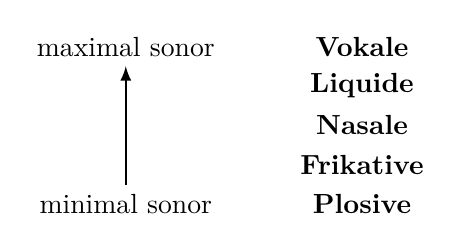
\begin{tikzpicture}
    \node (min)                             {minimal sonor};
    \node (plo) at ([shift={( 3,0)}]   min) {\textbf{Plosive}};
    \node (fri) at ([shift={( 0,0.5)}] plo) {\textbf{Frikative}};
    \node (nas) at ([shift={( 0,0.5)}] fri) {\textbf{Nasale}};
    \node (liq) at ([shift={( 0,0.5)}] nas) {\textbf{Liquide}};
    \node (vok) at ([shift={( 0,0.5)}] liq) {\textbf{Vokale}};
    \node (max) at ([shift={(-3,0)}]   vok) {maximal sonor};
    \draw [->, thick] (min) to (max);
  \end{tikzpicture}
  \caption{Sonoritätshierarchie}
  \label{fig:sonoritaet085}
\end{figure}

\begin{figure}[!htbp]
  \centering
  \begin{tikzpicture}
    \node (P1) at (0, 0.0) {P};
    \node (F1) at (1, 0.5) {F};
    \node (N1) at (2, 1.0) {N};
    \node (L1) at (3, 1.5) {L};
    \node (V0) at (4, 2.0) {V};
    \node (L2) at (5, 1.5) {L};
    \node (N2) at (6, 1.0) {N};
    \node (F2) at (7, 0.5) {F};
    \node (P2) at (8, 0.0) {P};
    \draw [->] (P1) to (F1);
    \draw [->] (F1) to (N1);
    \draw [->] (N1) to (L1);
    \draw [->] (L1) to (V0);
    \draw [->] (V0) to (L2);
    \draw [->] (L2) to (N2);
    \draw [->] (N2) to (F2);
    \draw [->] (F2) to (P2);
  \end{tikzpicture}
  \caption{Sonorität für die Segmentklassen in der schematischen Silbe}
  \label{fig:sonoritaet086}
\end{figure}

Innerhalb der Silbe gibt es das universelle Bildungsprinzip der \textit{Sonoritätskontur}, welches regelt, dass die Sonorität zum Vokal hin ansteigt und dann wieder abfällt, wie in Abbildung~\ref{fig:sonoritaet086} schematisch dargestellt.\index{Sonorität}
Eine Silbe, die nur aus einem Plosiv und einem Vokal besteht, zeigt einen Sonoritätsanstieg, aber keinen Sonoritätsabfall.
Es gibt also Silben, die nur einen Ausschnitt aus der Sonoritätskontur realisieren (nur Anstieg oder nur Abfall), aber einen Sonoritätsabfall gefolgt von einem Anstieg gibt es innerhalb einzelner Silben im Normalfall nicht.
Definition~\ref{def:sonoritaet} fasst zusammen.

\Definition{Sonorität und Sonoritätskontur}{\label{def:sonoritaet}%
Segmente können auf einer \textit{Sonoritätsskala} eingeordnet werden.
Alle zulässigen Silbenstrukturen stellen einen Anstieg der Sonorität zur Mitte der Silbe und einen Abfall der Sonorität zum Ende der Silbe (oder einen Ausschnitt aus einem solchen Verlauf) dar.
Sie weisen also eine steigende--fallende \textit{Sonoritätskontur} auf.
\index{Sonorität}
}

\Stretch[0.5]

\begin{exe}
  \ex\label{ex:sonoritaet087}
  \begin{xlist}
    \ex\label{ex:sonoritaet088} \textit{Kuh}\\[0.5\baselineskip]\leavevmode
      \SonDiag[2]{{k/\plo/0, u:/\vok/0}}\\[0.5\baselineskip]
\Stretch[0.5]
    \ex\label{ex:sonoritaet089} \textit{nie}\\[0.5\baselineskip]\leavevmode
      \SonDiag[2]{{n/\nas/0, i:/\vok/0}}\\[0.5\baselineskip]
\Stretch[0.5]
    \ex\label{ex:sonoritaet090} \textit{Knie}\\[0.5\baselineskip]\leavevmode
      \SonDiag[3]{{k/\plo/0, n/\nas/0, i:/\vok/0}}\\[0.5\baselineskip]
\Np
    \ex\label{ex:sonoritaet091} \textit{droh}\\[0.5\baselineskip]\leavevmode
      \SonDiag[3]{{d/\plo/0, ʁ/\liq/0, oː/\vok/0}}\\[0.5\baselineskip]
    \ex\label{ex:sonoritaet092} \textit{steh}\\[0.5\baselineskip]\leavevmode
      \SonDiag[3]{{ʃ/\fri/2, t/\plo/0, e:/\vok/0}}\\[0.5\baselineskip]
    \ex\label{ex:sonoritaet093} \textit{Schnee}\\[0.5\baselineskip]\leavevmode
      \SonDiag[3]{{ʃ/\fri/0, n/\nas/0, e:/\vok/0}}\\[0.5\baselineskip]
    \ex\label{ex:sonoritaet094} \textit{sprüh}\\[0.5\baselineskip]\leavevmode
      \SonDiag[4]{{ʃ/\fri/2, p/\plo/0, ʁ/\liq/0, y:/\vok/0}}\\[0.5\baselineskip]
    \ex\label{ex:sonoritaet095} \textit{ab}\\[0.5\baselineskip]\leavevmode
      \SonDiag[3]{{ʔ/\plo/0, a/\vok/0, p/\plo/0}}\\[0.5\baselineskip]
    \ex\label{ex:sonoritaet096} \textit{an}\\[0.5\baselineskip]\leavevmode
      \SonDiag[3]{{ʔ/\plo/0, a/\vok/0, n/\nas/0}}\\[0.5\baselineskip]
    \ex\label{ex:sonoritaet097} \textit{acht}\\[0.5\baselineskip]\leavevmode
      \SonDiag[4]{{ʔ/\plo/0, a/\vok/0, χ/\fri/0, t/\plo/0}}\\[0.5\baselineskip]
    \ex\label{ex:sonoritaet098} \textit{Alm}\\[0.5\baselineskip]\leavevmode
      \SonDiag[4]{{ʔ/\plo/0, a/\vok/0, l/\liq/0, m/\nas/0}}\\[0.5\baselineskip]
    \ex\label{ex:sonoritaet099} \textit{Raps}\\[0.5\baselineskip]\leavevmode
      \SonDiag[4]{{ʁ/\liq/0, a/\vok/0, p/\plo/0, s/\fri/2}}\\[0.5\baselineskip]
  \end{xlist}
\end{exe}

In (\ref{ex:sonoritaet087}) werden zur Illustration einige kurze einsilbige deutsche Wörter in \textit{Sonoritätsdiagrammen} in das Schema eingeordnet.
Das ideale Bild der Sonoritätskontur wird dabei weitgehend bestätigt.
Die einzige Ausnahme ist das Auftreten von den in den Diagrammen eingekreisten \textipa{[S]} vor Plosiven im Anfangsrand (\textit{sprüh}) und [s] nach Plosiven im Endrand (\textit{Raps}).
Da Frikative eine höhere Sonorität haben als Plosive, steigt in diesen Fällen die Sonorität zum Rand hin wieder an.
In Wörtern wie \textit{trittst} setzt sich das Problem sogar noch weiter fort, weil nach dem Anstieg ein weiterer Abfall folgt.
In \textit{Herbsts} folgt nach dem [p] sogar eine Kontur aus Anstieg, Abstieg und erneutem Anstieg, s.\ Abbildung~\ref{fig:sonoritaet100}.

\begin{figure}[!htbp]
  \centering
  \SonDiag[6]{{h/\fri/0, ɛ͡ə/\vok/0, p/\plo/0, s/\fri/2, t/\plo/2, s/\fri/2}}
  \caption{Sonorität am Beispiel von \textit{Herbsts}}
  \label{fig:sonoritaet100}
\end{figure}

Weil solche Sequenzen nicht der Sonoritätsbedingung entsprechen (sowie aus unabhängigen anderen Gründen, die in Abschnitt~\ref{sec:diesystematikderraender} und Abschnitt~\ref{sec:einsilblerundzweisilbler} erläutert werden), betrachten wir die betroffenen Segmente als \textit{extrasilbisch} (außerhalb der normalen Silbenstruktur stehend), vgl.\ Definition~\ref{def:extrasilbisch}.

\Definition{Extrasilbizität}{\label{def:extrasilbisch}\index{Extrasilbizität}%
Die Silbenstruktur kann durch extrasilbische Segmente ergänzt werden, die vor dem Anfangsrand oder nach dem Endrand stehen und nicht den Bedingungen der Sonoritätskontur unterliegen.}

Es ergibt sich eine erweiterte Silbenstruktur in Abbildung~\ref{fig:sonoritaet101}, in der die Sonoritätskontur nur für die Silbe, nicht aber für die mit gestrichelten Linien den Rändern angelehnten extrasilbischen Obstruenten gilt.
In einem Vorgriff auf Abschnitt~\ref{sec:diesystematikderraender} nehmen wir an, dass maximal zwei Konsonanten (C) im Anfangs- und Endrand stehen können, und dass vor dem Anfangsrand ein extrasilbisches Segment (X) und nach dem Endrand maximal drei extrasilbische Segmente stehen können.

\begin{figure}[!htbp]
  \centering
  \begin{forest}
    [Silbe, calign=last
      [Anfangsrand, sake, calign=child, calign child=2
        [X, edge=dashed][C][C]
      ]
      [Reim, calign=first
        [Kern, sake
          [V]
        ]
        [Endrand, sake, calign=child, calign child=2
          [C][C][X,edge=dashed][X,edge=dashed][X,edge=dashed]
        ]
      ]
    ]
  \end{forest}
  \caption{Schema für die Silbenstruktur mit extrasilbischen Segmenten}
  \label{fig:sonoritaet101}
\end{figure}

Außerdem kann die Sonorität auch gleich bleiben, so dass sich \textit{Plateaus} aus zwei Plosiven (\textit{Abt}), zwei Frikativen (\textit{Reichs}) usw.\ bilden.
Abbildung~\ref{fig:sonoritaet102} zeigt die Kontur des Wortes \textit{strolchst} mit extrasilbischem \textipa{[S]} vor dem Anfangsrand und einem Frikativ-Plateau im Endrand.
In Abschnitt~\ref{sec:diesystematikderraender} werden Plateaus allerdings eliminiert, indem plateaubildendes Material auch als extrasilbisch aufgefasst wird.

\begin{figure}[!htbp]
  \centering
  \SonDiag[8]{{ʃ/\fri/0, t/\plo/0, ʁ/\liq/0, ɔ/\vok/0, l/\liq/0, ç/\fri/0, s/\fri/0, t/\plo/0}}
  \caption{Sonorität am Beispiel von \textit{strolchst}}
  \label{fig:sonoritaet102}
\end{figure}

Was die Sonorität aus phonetisch-artikulatorischer oder perzeptorischer Sicht genau ist, ist eine schwierige Frage.
Stimmhaftigkeit ist ein wichtiger Faktor für eine hohe Sonorität.
Darüber hinaus kann als Faustregel gelten, dass, je enger die durch die Artikulatoren hergestellte Annäherung ist, die Sonorität umso geringer ist.
Dies entspricht dem artikulatorischen Schema des Öffnens und Schließens des Vokaltrakts (Abschnitt~\ref{sec:silben}).

\subsection{Die Systematik der Ränder}
\label{sec:diesystematikderraender}

\index{Silbe!Rand}

In diesem Abschnitt werden der Anfangsrand und der Endrand im Einsilbler für den Kernwortschatz mit dem Wissen um die Sonoritätshierarchie abschließend beschrieben.
Die Systematisierung des Anfangsrands wird dadurch erreicht, dass \textipa{[S]} in Anfangsrändern mit scheinbar zwei oder drei Segmenten eliminiert wird.%
\footnote{Typenseltene Wörter wie \textit{Skat} enthalten [s] statt \textipa{[S]}.
Wir zählen sie nicht zum Systemkern (s.\ Abschnitt~\ref{sec:kernundperipherie}).}
In Abschnitt~\ref{sec:sonoritaet} wurde festgestellt, dass \textipa{[S]} vor Plosiven (\textit{Sprung}, \textit{Stuhl}) die Sonoritätshierarchie verletzt.
Vor Frikativen (\textit{Schwung}) entsteht ein Sonoritätsplateau.
Lediglich in mehrsegmentalen Anfangsrändern mit einem Nasal oder Liquid an zweiter Stelle (\textit{Schmal}, \textit{Schrank}, \textit{Schlund}) verhält sich \textipa{[S]} theoretisch konform zur Sonoritätshierarchie.
Zudem sind die einzigen Anfangsränder mit drei Segmenten solche, bei denen das erste Segment \textipa{[S]} ist.
Das Segment \textipa{[S]} verhält sich im Silbenbau offensichtlich besonders, und es wurde mit Definition~\ref{def:extrasilbisch} aus der eigentlichen Silbe in einen erweiterten Bereich verschoben, in dem die Sonoritätskontur nicht eingehalten werden muss.
Es ist \textit{extrasilbisch}.

\begin{figure}[!htbp]
  \centering
  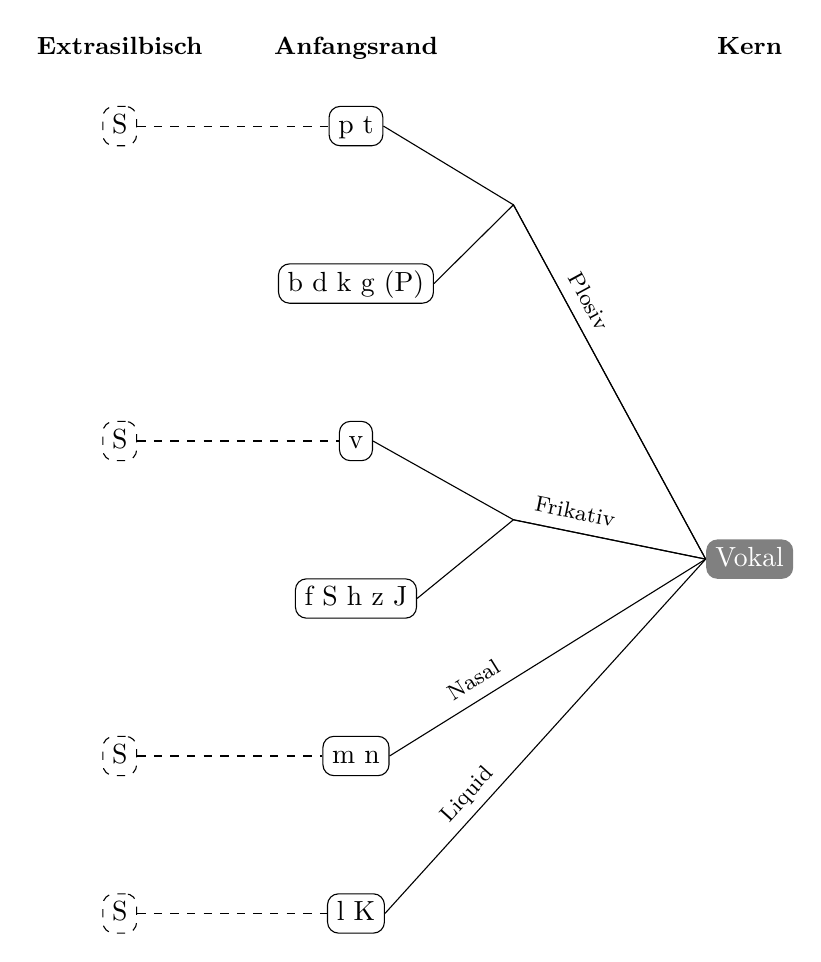
\begin{tikzpicture}[text height=1.5ex, text depth=.25ex, text centered]
    \tikzset{%
      segm/.style={fill=white, draw, rounded corners, execute at begin node=\tipaencoding},
      extrasyl/.style={segm, dashed}
      }
    \node at (0, 12) {\textbf{\small Extrasilbisch}};
    \node at (3, 12) {\textbf{\small Anfangsrand}};
    \node at (8, 12) {\textbf{\small Kern}};

    \node [fill=gray, rounded corners] (Xvok) at (8, 5.5) {\textcolor{white}{Vokal}};

    \node [segm] (Xplu) at (3,11) {p t};
    \node [extrasyl] (XSplu) at (0,11) {S};
    \draw [dashed] (XSplu) to (Xplu);
    \node [segm] (Xplv) at (3,9) {b d k g (P)};
    \draw (Xvok.west) -- node [pos=0.7, above, sloped] {\footnotesize Plosiv} (5, 10) -- (Xplu.east);
    \draw (Xvok.west) -- (5, 10) -- (Xplv.east);

    \node [segm] (Xvov) at (3,7) {v};
    \node [extrasyl] (XSvov) at (0,7) {S};
    \draw [dashed] (XSvov) to (Xvov);
    \node [segm] (Xfri) at (3,5) {f S h z J};
    \draw (Xvok.west) -- node [pos=0.7, above, sloped] {\footnotesize Frikativ} (5, 6) -- (Xvov.east);
    \draw (Xvok.west) -- (5, 6) -- (Xfri.east);

    \node [segm] (Xnas) at (3,3) {m n};
    \node [extrasyl] (XSnas) at (0,3) {S};
    \draw [dashed] (XSnas) to (Xnas);
    \node [segm] (Xliq) at (3,1) {l K};
    \node [extrasyl] (XSliq) at (0,1) {S};
    \draw [dashed] (XSliq) to (Xliq);
    \draw (Xvok.west) to node [pos=0.7, above, sloped] {\footnotesize Nasal} (Xnas.east);
    \draw (Xvok.west) to node [pos=0.7, above, sloped] {\footnotesize Liquid} (Xliq.east);
  \end{tikzpicture}
  \caption{Struktur des simplexen Anfangsrands}
  \label{fig:diesystematikderraender103}
\end{figure}

Die maximale Komplexität des Anfangsrands besteht also in zwei Segmenten:\index{Silbe!Anfangsrand!komplex}
Der Anfangsrand ist maximal \textit{duplex}.
Scheinbare Fälle von drei Segmenten im Anfangsrand (\textipa{[SpK]}, \textipa{[StK]} und evtl.\ \textipa{[Spl]}) im Anfangsrand bestehen aus zwei Segmenten mit extrasilbischem \textipa{[S]}.
Wenn man \textipa{[S]} diesen Sonderstatus zuweist, dampft die Beschreibung der Besetzungsmöglichkeiten des simplexen Anfangsrands auf Abbildung~\ref{fig:diesystematikderraender103} und die des duplexen Anfangsrands auf Abbildung~\ref{fig:diesystematikderraender104} ein.
Die Abbildungen sind von rechts nach links zu lesen, und sie bilden die \textit{Besetzungsmöglichkeiten} des Anfangsrands ab.
Für jede mögliche Besetzung des Anfangsrands gibt es genau einen Weg durch die Äste des Diagramms.
Man beginnt mit dem Vokal im Kern.
Die von dort nach links weisenden Äste zeigen Besetzungsmöglichkeiten für das erste Segment im Anfangsrand links vom Vokal.
Von diesen weisen ggf.\ weitere Äste nach links, die die Möglichkeiten für weiter links stehende Segmente anzeigen, und zwar abhängig von dem bereits eingeschlagenen Weg.
Die in Gruppen angeordneten Segmente stellen jeweils verschiedene Möglichkeiten der Besetzung dar.
In Abbildung~\ref{fig:diesystematikderraender103} kann man vor dem Vokal zum Beispiel einen Plosiv einsetzen (oberer Ast).
Es kommen \textipa{[p]} oder \textipa{[t]} infrage (obere Verästelung des obersten Asts), vor dem noch ein \textipa{[S]} stehen kann.
Vor \textipa{[b]}, \textipa{[d]}, \textipa{[k]} und \textipa{[g]} (untere Verästelung des oberen Asts) kann allerdings kein \textipa{[S]} stehen.
Der Glottalplosiv \textipa{[P]} ist eingeklammert, um seinen Sonderstatus als nicht zugrundeliegendes Segment zu markieren.

Es wird sofort deutlich, dass die Kombinationsmöglichkeiten sehr stark auf die Verbindung von Plosiven oder den labiodentalen Frikativen [f] und [v] mit folgendem Liquid eingeschränkt sind.
Zwischen den beiden Liquiden an zweiter Stelle gibt es im Wesentlichen zwei minimale Unterschiede.
Einerseits kommen die Kombinationen \textipa{[tK]} (\textit{Trog}) und \textipa{[dK]} (\textit{Druck}), nicht aber die Kombinationen \textipa{[tl]} und \textipa{[dl]} vor.%
\footnote{Diese Einschränkung kann man damit erklären, dass \textipa{[l]} den gleichen Artikulationsort wie \textipa{[t]} und \textipa{[d]} hat, und dass die Segmente dadurch zu ähnlich sind, um im Anfangsrand zusammen vorzukommen.
Eine \textit{Erklärung} im Sinne einer kausalen Beziehung wird daraus allerdings ohne erheblichen argumentativen Mehraufwand und Zusatzannahmen nicht, zumal an anderer Stelle (bei Assimilationen) sogar eine Angleichung von Artikulationsorten gefordert wird.}
Andererseits ist \textipa{[vK]} möglich (\textit{wringen}), aber (im Kern des Systems) nicht \textipa{[vl]} (vgl.\ aber peripher \textit{Vladimir} usw.).
In Satz~\ref{satz:anfangsrand} wird die Struktur des Anfangsrands kompakt beschrieben.

\Satz{Anfangsrand}{\label{satz:anfangsrand}%
Der Anfangsrand ist maximal duplex.
Die präferierte Besetzung des duplexen Anfangsrands ist die aus einem inneren Liquid und einem äußeren Obstruenten.
Extrasilbisch tritt ggf.\ \textipa{[S]} vor den Anfangsrand.\index{Silbe!Anfangsrand!komplex}}

\begin{figure}[!htbp]
  \centering
  \resizebox{!}{0.95\textheight}{
  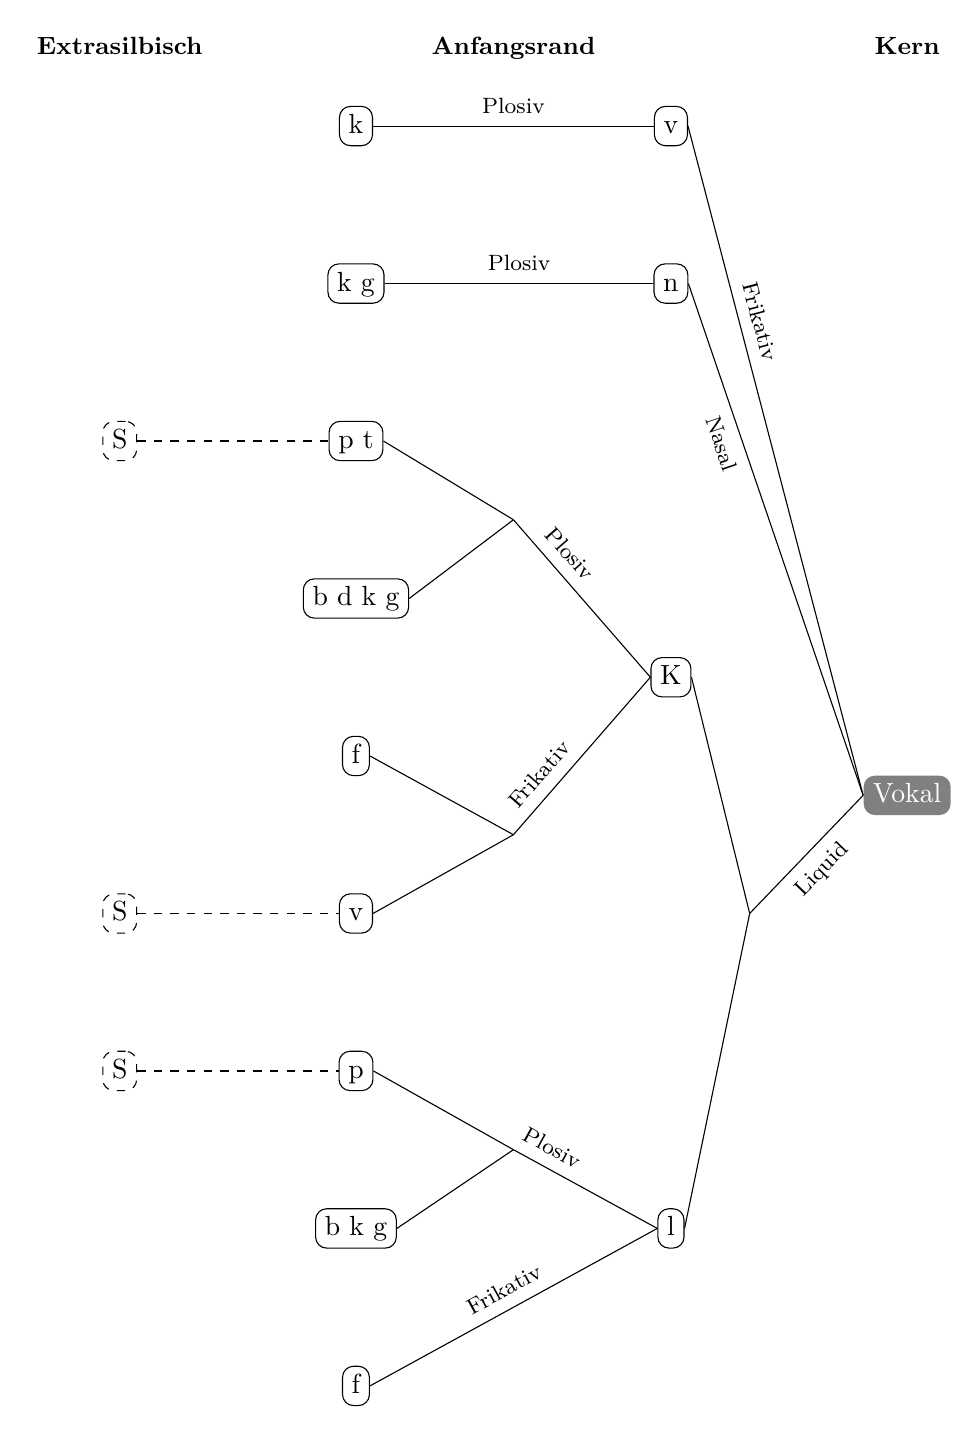
\begin{tikzpicture}[text height=1.5ex, text depth=.25ex, text centered]
    \tikzset{%
      segm/.style={fill=white, draw, rounded corners, execute at begin node=\tipaencoding},
      extrasyl/.style={segm, dashed}
      }
    \node at (0, 18) {\textbf{\small Extrasilbisch}};
    \node at (5, 18) {\textbf{\small Anfangsrand}};
    \node at (10, 18) {\textbf{\small Kern}};

    \node [fill=gray, rounded corners] (Yvok) at (10, 8.5) {\textcolor{white}{Vokal}};

    \node [segm] (Yk) at (3,17) {k};
    \node [segm] (Yv) at (7,17) {v};
    \draw (Yk.east) -- node [pos=0.5, above] {\footnotesize Plosiv} (Yv.west);
    \draw (Yvok.west) -- node [pos=0.7, above, sloped] {\footnotesize Frikativ} (Yv.east);

    \node [segm] (Ykg) at (3,15) {k g};
    \node [segm] (Yn) at (7,15) {n};
    \draw (Ykg.east) -- node [pos=0.5, above] {\footnotesize Plosiv} (Yn.west);
    \draw (Yvok.west) -- node [pos=0.7, below, sloped] {\footnotesize Nasal} (Yn.east);

    \node [segm] (Ypt) at (3,13) {p t};
    \node [extrasyl] (YSpt) at (0,13) {S};
    \draw [dashed] (YSpt) to (Ypt);
    \node [segm] (Ybdkg) at (3,11) {b d k g};
    \node [segm] (Yf) at (3,9) {f};
    \node [segm] (Yv1) at (3,7) {v};
    \node [extrasyl] (YSv1) at (0,7) {S};
    \draw [dashed] (YSv1) to (Yv1);

    \node [segm] (YR) at (7,10) {K};
    \draw (Ypt.east) -- (5,12);
    \draw (Ybdkg.east) -- (5,12);
    \draw (5,12) -- node [pos=0.3, above, sloped] {\footnotesize Plosiv} (YR.west);
    \draw (Yf.east) -- (5,8);
    \draw (Yv1.east) -- (5,8);
    \draw (5,8) -- node [pos=0.3, above, sloped] {\footnotesize Frikativ} (YR.west);

    \node [segm] (Yp) at (3,5) {p};
    \node [extrasyl] (YSp) at (0,5) {S};
    \draw [dashed] (YSp) to (Yp);
    \node [segm] (Ybkg) at (3,3) {b k g};
    \node [segm] (Yff) at (3,1) {f};

    \node [segm] (Yl) at (7,3) {l};
    \draw (Yp.east) -- (5,4);
    \draw (Ybkg.east) -- (5,4);
    \draw (5,4) -- node [pos=0.2, above, sloped] {\footnotesize Plosiv} (Yl.west);
    \draw (Yff.east) -- node [pos=0.5, above, sloped] {\footnotesize Frikativ} (Yl.west);

    \draw (YR.east) -- (8,7);
    \draw (Yl.east) -- (8,7);
    \draw (8,7) -- node [pos=0.5, below, sloped] {\footnotesize Liquid} (Yvok.west);

  \end{tikzpicture}}
  \caption{Struktur des duplexen Anfangsrands}
  \label{fig:diesystematikderraender104}
\end{figure}

Bei der deskriptiven Sichtung in Abschnitt~\ref{sec:derendrandimeinsilbler} schien der Endrand drei oder mehr Segmente enthalten zu können.\index{Silbe!Endrand!komplex}
Wir beschreiben jetzt zunächst den duplexen Endrand und versuchen, davon ausgehend weiter zu systematisieren.
Alle Kombinationen, die eine Verletzung der Sonoritätskontur darstellen würden, werden dabei gleich ausgeschlossen.
Außerdem wird \textipa{[N]} als zugrundeliegendes Segment aus dem System eliminiert (mehr dazu weiter unten).
Es ergibt sich Abbildung~\ref{fig:diesystematikderraender105}, die den duplexen Endrand ohne extrasilbisches Material abbildet.

\begin{figure}[!htbp]
  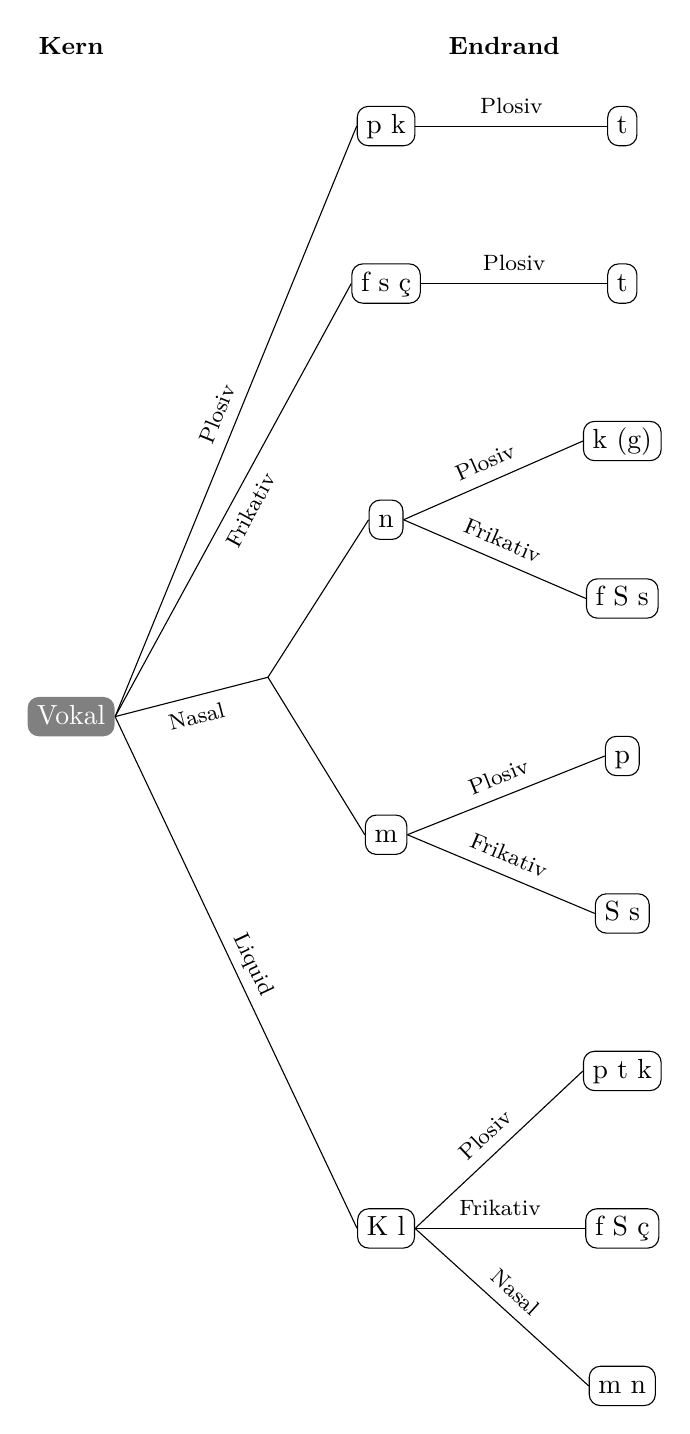
\begin{tikzpicture}[text height=1.5ex, text depth=.25ex, text centered]
    \tikzset{%
      segm/.style={fill=white, draw, rounded corners, execute at begin node=\tipaencoding},
      extrasyl/.style={segm, dashed}
      }
     \node at (-1, 18) {\textbf{\small Kern}};
     \node at (4.5, 18) {\textbf{\small Endrand}};

     \node [fill=gray, rounded corners] (Zvok) at (-1, 9.5) {\textcolor{white}{Vokal}};
     
     \node [segm] (Ot) at (6, 17) {t};
     \node [segm] (pk) at (3, 17) {p k};
     \draw (pk.east) -- node [pos=0.5, above, sloped] {\footnotesize Plosiv} (Ot.west);
     \draw (Zvok.east) --  node [pos=0.5, above, sloped] {\footnotesize Plosiv} (pk.west);

     \node [segm] (t) at (6, 15) {t};
     \node [segm] (fs) at (3, 15) {f s \c{c}};
     \draw (fs.east) -- node [pos=0.5, above, sloped] {\footnotesize Plosiv} (t.west);
     \draw (Zvok.east) --  node [pos=0.5, below, sloped] {\footnotesize Frikativ} (fs.west);

     \node [segm] (Zkg) at (6,13) {k (g)};
     \node [segm] (ZfSs) at (6,11) {f S s};

     \node [segm] (Zn) at (3,12) {n};
     \draw (Zn.east) -- node [pos=0.5, above, sloped] {\footnotesize Plosiv} (Zkg.west);
     \draw (Zn.east) -- node [pos=0.5, above, sloped] {\footnotesize Frikativ} (ZfSs.west);

     \node [segm] (Zp) at (6,9) {p};
     \node [segm] (ZSs) at (6,7) {S s};

     \node [segm] (Zm) at (3,8) {m};
     \draw (Zm.east) -- node [pos=0.5, above, sloped] {\footnotesize Plosiv} (Zp.west);
     \draw (Zm.east) -- node [pos=0.5, above, sloped] {\footnotesize Frikativ} (ZSs.west);

     \draw (Zvok.east) --  node [pos=0.5, below, sloped] {\footnotesize Nasal} (1.5,10);
     \draw (1.5,10) -- (Zn.west);
     \draw (1.5,10) -- (Zm.west);

     \node [segm] (Zpk) at (6,5) {p t k};
     \node [segm] (ZfSc) at (6,3) {f S ç};
     \node [segm] (Zmn) at (6,1) {m n};

     \node [segm] (ZRl) at (3,3) {K l};
     \draw (ZRl.east) -- node [pos=0.5, above, sloped] {\footnotesize Plosiv} (Zpk.west);
     \draw (ZRl.east) -- node [pos=0.5, above, sloped] {\footnotesize Frikativ} (ZfSc.west);
     \draw (ZRl.east) -- node [pos=0.5, above, sloped] {\footnotesize Nasal} (Zmn.west);

     \draw (Zvok.east) -- node [pos=0.5, above, sloped] {\footnotesize Liquid} (ZRl.west);

  \end{tikzpicture}
  \caption{Struktur des duplexen Endrands}
  \label{fig:diesystematikderraender105}
\end{figure}

Das Diagramm in Abbildung~\ref{fig:diesystematikderraender105} beschreibt nicht alle Endränder, die rein oberflächlich gesehen duplex sind.
Wir betrachten diese Fälle -- also (\ref{ex:diesystematikderraender107}) -- hier zusammen mit Sonoritätsplateaus im Endrand, also insgesamt (\ref{ex:diesystematikderraender106}).

\begin{exe}
  \ex \label{ex:diesystematikderraender106}
  \begin{xlist}
    \ex{\label{ex:diesystematikderraender107} Huts, Schnaps}
    \ex{\label{ex:diesystematikderraender108} legt, nackt}
    \ex{\label{ex:diesystematikderraender109} Laufs, Krachs}
  \end{xlist}
\end{exe}

Die Wörter in (\ref{ex:diesystematikderraender107}) enthalten ein [s], das die Sonoritätskontur verletzt.
Wie schon im Anfangsrand behandeln wir alle Segmente prinzipiell als extrasilbisch, wenn sie die Sonoritätskontur verletzen.
In Fällen mit scheinbar drei Segmenten im Endrand wie \textit{trittst} muss [t] dann auch extrasilbisch sein, da das vorangehende [s] bereits extrasilbisch ist.
Es ist zu beachten, dass sowohl [t] als auch [s] und \textipa{[S]} alveolare Obstruenten sind, und damit eine (wenn auch kleine) homogene Klasse bilden.
Wir nehmen daher an, dass nur alveolare Obstruenten extrasilbisch auftreten.

Einfache Wörter mit Sonoritätsplateaus aus zwei Plosiven im Endrand wie \textit{nackt} aus (\ref{ex:diesystematikderraender108}) sind höchst selten und nur mit \textipa{[t]} an zweiter Position möglich.
Wir behandeln die entsprechenden \textipa{[t]}-Segmente nur dann als extrasilbisch, \textit{wenn der Vokal im Kern lang ist}.
Die Zusatzbedingung der Vokallänge findet ihre Begründung in der Analyse des sogenannten \textit{Silbengewichts} und wird in Abschnitt~\ref{sec:einsilblerundzweisilbler} genauer motiviert.
Es wird dort gezeigt werden, dass deutsche Silben systematisch entweder aus einem kurzen Kern und einem duplexen Endrand oder einem langen Kern und einem simplexen Endrand bestehen.
Das ein Plateau bildende [s] in (\ref{ex:diesystematikderraender109}) wird parallel dazu nur dann als extrasilbisch analysiert, wenn der Vokal im Kern lang (hier der Diphthong in \textit{Laufs}) ist.

Insgesamt eliminieren wir durch die Annahme von extrasilbischen [t]- und [s]-Seg\-men\-ten alle Endränder mit mehr als zwei Segmenten vollständig aus dem System.
Das System wird so simpel, wie es in Abbildung~\ref{fig:diesystematikderraender105} aussieht.
Die Beziehung von zugrundeliegender Form und phonetischer Oberfläche wird in den Analysen in (\ref{ex:diesystematikderraender110}) verdeutlicht, wo extrasilbische Segmente mit + abgetrennt wurden.

\begin{exe}
  \ex \label{ex:diesystematikderraender110}
  \begin{xlist}
    \ex{\label{ex:diesystematikderraender111} /\textipa{huts}/ $\Rightarrow$ \textipa{[hu:t+s]} (\textit{Huts})}
    \ex{\label{ex:diesystematikderraender112} /\textipa{Sn\u{a}ps}/ $\Rightarrow$ \textipa{[S+nap+s]} (\textit{Schnaps})}
    \ex{\label{ex:diesystematikderraender113} /\textipa{legt}/ $\Rightarrow$ \textipa{[le:k+t]} (\textit{legt})}
    \ex{\label{ex:diesystematikderraender114} /\textipa{n\u{a}kt}/ $\Rightarrow$ \textipa{[nakt]} (\textit{nackt})}
    \ex{\label{ex:diesystematikderraender115} /\textipa{l\t{aO}fs}/ $\Rightarrow$ \textipa{[l\t{aO}f+s]} (\textit{Laufs})}
    \ex{\label{ex:diesystematikderraender116} /\textipa{kK\u{a}Xs}/ $\Rightarrow$ \textipa{[kKaXs]} (\textit{Krachs})}
  \end{xlist}
\end{exe}

Die Kombinationen aus Frikativ und [t] können theoretisch auch als simplexe Endränder mit extrasilbischem [t] aufgefasst werden.
Wir tun dies parallel zur Behandlung der Plateaus aber wieder nur dann, wenn der Vokal im Kern lang ist.
Die sich ergebenden Formen zeigt (\ref{ex:diesystematikderraender117}).

\begin{exe}
  \ex \label{ex:diesystematikderraender117}
  \begin{xlist}
    \ex{\label{ex:diesystematikderraender118} /\textipa{Kuft}/ $\Rightarrow$ \textipa{[Ku:f+t]} (\textit{ruft})}
    \ex{\label{ex:diesystematikderraender119} /\textipa{\u{a}\c{c}t}/ $\Rightarrow$ \textipa{[PaXt]} (\textit{Acht})}
    \ex{\label{ex:diesystematikderraender120} /\textipa{lest}/ $\Rightarrow$ \textipa{[le:s+t]} (\textit{lest})}
    \ex{\label{ex:diesystematikderraender999} /\textipa{l\u{E}st}/ $\Rightarrow$ \textipa{[lEst]} (\textit{lässt})}
  \end{xlist}
\end{exe}

Abschließend bleiben noch zwei Merkwürdigkeiten in Abbildung~\ref{fig:diesystematikderraender105} zu erklären, die in Endrändern mit Nasal als erstes Segment auftreten.
Einerseits fehlt \textipa{[N]} vollständig, andererseits kommt nach [n] angeblich ein [g] vor, wobei dieses in Abbildung~\ref{fig:diesystematikderraender105} eingeklammert ist.
Im Endrand sollte schließlich aufgrund der Endrand-Desonorisierung kein stimmhafter Plosiv vorkommen können.

Mögliche zweisegmentale Endränder mit velarem Nasal \textipa{[N]} an der phonetischen Oberfläche findet man in Wörtern mit nachfolgendem velaren Plosiv wie \textit{krank} \textipa{[kKaNk]}.
Es fällt insgesamt auf, dass zwar [t] mit allen Nasalen kombiniert werden kann (\textit{klemmt}, \textit{rennt}, \textit{hängt}), [p] aber nur mit [m] (\textit{Lump}) und [k] nur mit \textipa{[N]} (\textit{krank}).
Es liegt der Verdacht nahe, dass hier eigentlich nur homorgane (am selben Ort artikulierte) Sequenzen aus Nasal und Plosiv vorkommen können.
Wir gehen also von /\textipa{kKank}/ \phopro \textipa{[kKaNk]} und /\textipa{lUnp}/ \phopro \textipa{[lUmp]} aus.
Ein [t] nach [m] oder \textipa{[N]} wie in \textit{klemmt} oder \textit{hängt} ist dann als extrasilbisch zu analysieren.

Was ist aber mit dem einfachen \textipa{[N]} wie in \textit{Gang}?
Hier folgt dem velaren Nasal kein velarer Plosiv, an den er seinen Artikulationsort anpassen könnte.
Wir führen \textipa{[N]} auf eine zugrundeliegende Kombination /ng/ zurück.
Der Nasal /n/ assimiliert an /g/ zu \textipa{[N]}, und das /g/ wird nicht artikuliert.
Phonologisch und aus Sicht der Silbifizierung haben wir es \zB in /gang/ also mit einem duplexen Endrand zu tun, phonetisch mit einem simplexen.
Weil es phonetisch nach /n/ im Endrand niemals auftritt, ist \textipa{[g]} in Abbildung~\ref{fig:diesystematikderraender105} eingeklammert.
Außerdem können wir dank der Analyse von \textipa{[N]} als /ng/ das Segment \textipa{[N]} als zugrundeliegendes Segment vollständig eliminieren.
Deswegen wird es hier konsequent in [~] statt in /~/ geschrieben.
Für diese Reduktion des Systems wird in Abschnitt~\ref{sec:einsilblerundzweisilbler} weiter argumentiert, da sich \textipa{[N]} als phonetisches Korrelat zu /ng/ im Endrand auch bezüglich des Silbengewichts wie zwei Segmente verhält:
In Silben, die auf /ng/ enden, kann der Vokal niemals lang (bzw.\ ein Diphthong) sein.

Die Beziehung zugrundeliegender Formen und ihrer phonetischen Realisierungen in einigen Formen illustriert (\ref{ex:diesystematikderraender121}).
Beispiel (\ref{ex:diesystematikderraender127}) wird gegeben, um zu illustrieren, dass nicht alle \textipa{[t]}-Segmente nach Nasal extrasilbisch sein müssen.

\begin{exe}
  \ex \label{ex:diesystematikderraender121}
  \begin{xlist}
    \ex{\label{ex:diesystematikderraender122} /\textipa{g\u{a}ng}/ $\Rightarrow$ \textipa{[gaN]} (\textit{Gang})}
    \ex{\label{ex:diesystematikderraender123} /\textipa{l\u{E}ngs}/ $\Rightarrow$ \textipa{[lEN+s]} (\textit{längs})}
    \ex{\label{ex:diesystematikderraender124} /\textipa{h\u{E}ngt}/ $\Rightarrow$ \textipa{[hEN+t]} (\textit{hängt})}
    \ex{\label{ex:diesystematikderraender125} /\textipa{kr\u{a}nk}/ $\Rightarrow$ \textipa{[kraNk]} (\textit{krank})}
    \ex{\label{ex:diesystematikderraender126} /\textipa{kl\u{E}mt}/ $\Rightarrow$ \textipa{[klEm+t]} (\textit{klemmt})}
    \ex{\label{ex:diesystematikderraender127} /\textipa{bUnt}/ $\Rightarrow$ \textipa{[bUnt]} (\textit{bunt})}
  \end{xlist}
\end{exe}

Es fällt außerdem auf, dass häufig -- wenn auch nicht immer -- extrasilbisches Material (konkret [t], [s] oder [st]) zu sogenannten \textit{Flexionsendungen} gehört, also nicht zum sogenannten \textit{Wortstamm} (vgl.\ Abschnitt~\ref{sec:woerterwortformenundstaemme}).\index{Extrasilbizität!und Flexionssuffixe}
Mit der Grenze zwischen echtem Endrand und extrasilbischem Material fällt also oft auch die Grenze zwischen Stamm und Flexionsendung zusammen, \zB \textit{lebst} \textipa{[le:p+st]}, \textit{glaubt} \textipa{[gl\t{aO}p+t]} oder \textit{Stifts} \textipa{[StIft+s]}.

Zusammenfassend kann man -- wie schon in umgekehrter Reihenfolge beim Anfangsrand -- festhalten, dass der prototypische duplexe Endrand aus einem innerem Liquid und einem äußerem Obstruenten besteht.
Dem Endrand nachfolgende [s] und [t] sind als extrasilbisch zu werten.
In (\ref{ex:diesystematikderraender128}) finden sich weitere Beispiele, wobei (\ref{ex:diesystematikderraender129}) als Referenzbeispiel ohne extrasilbische Konsonanten angegeben wird.%
\footnote{Bezüglich der Realisierung von /\textipa{K}/ als Vokal sollte an dieser Stelle ggf.\ Abschnitt~\ref{sec:orthographischesr} wiederholt werden.}

\Enl[2]

\begin{exe}
  \ex \label{ex:diesystematikderraender128}
  \begin{xlist}
    \ex{\label{ex:diesystematikderraender129} /\textipa{kOKb}/ $\Rightarrow$ \textipa{[k\t{O@}p]} (\textit{Korb})}
    \ex{\label{ex:diesystematikderraender130} /\textipa{vIKbst}/ $\Rightarrow$ \textipa{[v\t{I@}p+st]} (\textit{wirbst})}
    \ex{\label{ex:diesystematikderraender131} /\textipa{fUK\c{c}t}/ $\Rightarrow$ \textipa{[f\t{U@}\c{c}+t]} (\textit{Furcht})}
    \ex{\label{ex:diesystematikderraender132} /\textipa{f\u{E}lSst}/ $\Rightarrow$ \textipa{[fElS+st]} (\textit{fälschst})}
  \end{xlist}
\end{exe}

Vor einer weiteren Vertiefung der strukturellen Zusammenhänge, die in Abschnitt~\ref{sec:einsilblerundzweisilbler} erfolgen wird, halten wir in Satz~\ref{satz:endrandbesetzung} fest, dass die Besetzungspräferenzen im Endrand nahezu spiegelbildlich dieselben wie im Anfangsrand sind.%
\footnote{Als echte Auslassung im Interesse einer eleganteren Darstellung wurde in Abbildung~\ref{fig:diesystematikderraender105} die Besetzung des Endrands aus zugrundeliegendem /\textipa{Kl}/ wie in \textit{Kerl} unterschlagen.
Diese ist im Anfangsrand weder in dieser Reihenfolge noch spiegelbildlich zulässig.
Es drängt sich der Gedanke auf, dass diese Besetzung deshalb möglich ist, weil hier /\textipa{K}/ als zweites Element in einem sekundären Diphthong artikuliert wird, also /\textipa{k\u{E}Kl}/ \phopro \textipa{[k\t{E@}l]}.
Im Grunde stellen wir damit die Frage, ob das zweite Element von sekundären und ggf. auch primären Diphthongen eine Position im Kern oder im Endrand besetzt.
Eine zufriedenstellende Analyse solcher komplexer Bedingungen ist meiner Ansicht nur in formal ausgearbeiteten Theorien möglich.}

\Satz{Endrand}{\label{satz:endrandbesetzung}\index{Silbe!Endrand!komplex}%
Der Endrand ist maximal duplex.
Die präferierte Besetzung des duplexen Endrands ist die aus einem inneren Liquid und einem äußeren Obstruenten.
Bereits weniger präferiert wird er mit einem Nasal und einem homorganen Plosiv besetzt.
Extrasilbisch treten die alveolaren Obstruenten [s] und [t] an den Endrand.}

\subsection{Einsilbler und Zweisilbler}
\label{sec:einsilblerundzweisilbler}

\index{Silbe!Silbifizierung}
\index{Einsilbler}
\index{Zweisilbler}

Nach den Silben ist die nächstgrößere Einheit der phonologischen Strukturbildung das \textit{phonologische Wort}.
Der Grund, warum man eine solche Einheit annehmen möchte, ist, dass es phonologische Regularitäten gibt, die sich nicht nur mit Bezug auf Segmente und einzelne Silben beschreiben lassen, vgl.\ Definition~\ref{def:phonwort}.%
\footnote{Es müsste eigentlich der \textit{Fuß} als nächstgrößere Einheit nach der Silbe definiert werden.
Wir gehen nur in Abschnitt~\ref{sec:wortakzentimdeutschen} kurz auf den Fuß ein und wählen daher hier eine vereinfachte Darstellung.}

\Definition{Phonologisches Wort}{\label{def:phonwort}%
Ein \textit{phonologisches Wort} ist die kleinste phonologische Struktur, die Silben als Konstituenten hat, und bezüglich derer eigene Regularitäten feststellbar sind.
\index{Wort!phonologisch}
}

Definition~\ref{def:phonwort} kommt sehr formal daher.
Denken wir aber an den Grammatikbegriff aus Definition~\ref{def:grammatik} (Seite~\pageref{def:grammatik}), dann ist die Einschränkung \textit{bezüglich derer eigene Regularitäten feststellbar sind} aber ausgesprochen instruktiv.
Wenn es nämlich phonologische Regularitäten gibt, die sich nicht effektiv und angemessen mit Bezug auf Segmente und Silben beschreiben lassen, müssen wir eine andere, größere Einheit annehmen, bezüglich derer wir sie beschreiben können.
Eine solche Regularität wird im Rest dieses Abschnitts ausführlich analysiert.
Zunächst wird dazu der Sprachgebrauch von der \textit{offenen} und der \textit{geschlossenen Silbe} in Definition~\ref{def:offengeschlossen} eingeführt, der die weitere Argumentation vereinfacht.

\Definition{Offene und geschlossene Silben}{\label{def:offengeschlossen}%
Silben mit gefülltem Endrand sind \textit{geschlossene Silben}, Silben mit leerem Endrand sind \textit{offene Silben}.
\index{Silbe!offen}
\index{Silbe!geschlossen}
}

Wir beginnen mit einer Liste von instruktiven Beispielen in (\ref{ex:einsilblerundzweisilbler133}). 
Im Sinn einer übersichtlichen Darstellung beschränken wir uns hier auf die Vokale \textipa{[I]} und \textipa{[i]}, aber die Regularitäten gelten für alle Paare von ungespannten und gespannten Vokalen.

\begin{exe}
  \ex\label{ex:einsilblerundzweisilbler133}
  \begin{xlist}
    \ex[ ]{\label{ex:einsilblerundzweisilbler134} Knie \textipa{[kni:]}}
    \ex[*]{\label{ex:einsilblerundzweisilbler135} \textipa{[knI]}}
    \ex[ ]{\label{ex:einsilblerundzweisilbler136} schief \textipa{[Si:f]}}
    \ex[ ]{\label{ex:einsilblerundzweisilbler137} Schiff \textipa{[SIf]}}
    \ex[ ]{\label{ex:einsilblerundzweisilbler138} Wink \textipa{[vINk]}}
    \ex[*]{\label{ex:einsilblerundzweisilbler139} \textipa{[vi:Nk]}}
    \ex[*]{\label{ex:einsilblerundzweisilbler140} \textipa{[Pa:lt]}}
    \ex[ ]{\label{ex:einsilblerundzweisilbler141} Mie.te \textipa{[mi:.t@]}}
    \ex[ ]{\label{ex:einsilblerundzweisilbler142} Mi.tte \textipa{[mI.t@]}}
    \ex[ ]{\label{ex:einsilblerundzweisilbler143} liebte \textipa{[li:p.t@]}}
  \end{xlist}
\end{exe}

Die Wörter in (\ref{ex:einsilblerundzweisilbler133}) sind allesamt endungslos (also nicht nach Kasus, Person usw.\ flektiert) und damit sogenannte \textit{Simplizia}.\index{Simplex}
Zum Teil sind sie Einsilbler, zum Teil sind sie Zweisilbler, die aus einer Silbe mit einem betonten gespannten (langen) oder einem betonten ungespannten (kurzen) Vokal sowie einer Schwa-Silbe bestehen.
Diese beiden Muster der Silbenfolge sind charakteristisch für das Deutsche und grenzen den Kernwortschatz ein (s.\ auch Abschnitt~\ref{sec:wortakzentimdeutschen}).\index{Kern!Wortschatz}
Die folgende Argumentation betrachtet sie dementsprechend als Kern des phonologischen Systems:
Das einsilbige Simplex ist damit das Muster der Silbe an sich, und das Verhalten von Silben im zweisilbigen Simplex ist das Muster für Silben in Mehrsilblern.
Alle anderen Fälle und Erweiterungen werden durch entsprechend erweiterte Regularitäten beschrieben.
Uns interessiert jetzt hier vor allem die Silbenstruktur in der jeweils ersten Silbe bzw.\ der einzigen Silbe in diesen Wörtern.
Als zweite Silbe kommen hier nur Schwa-Silben vor, die von den zu beschreibenden Regularitäten als einzige nicht betroffen sind, weil sie prinzipiell nicht betonbar sind.
Es geht also ganz präzise gesagt um \textit{betonbare Silbentypen in ein- und zweisilbigen Simplizia des Kernwortschatzes}.

Einsilbige Simplizia mit ungespanntem Vokal müssen geschlossen sein, \zB \textit{Schiff} im Vergleich mit unmöglichen Wörtern wie *\textipa{[knI]} oder auch *\textipa{[tO]} usw.
Das gilt auch für die letzte Silbe in Mehrsilblern, weswegen *\textipa{[kUn.dI]} oder *\textipa{[tu:.bO]} keine möglichen Wörter des Deutschen sind.
Die einzige Ausnahme bilden Schwa-Silben, die offen als Endsilbe im Mehrsilbler vorkommen können, vgl.\ \textit{Mitte} \textipa{[mi.t@]}.
Wenn der Vokal gespannt ist, kann die Silbe offen sein wie in \textit{Knie}, muss sie aber nicht, vgl.\ \textit{schief}.
Wenn der Endrand des simplexen Einsilblers duplex ist wie in \textit{Wink} oder \textit{alt}, sind gespannte Vokale nicht möglich.
Die strukturell unmöglichen Simplizia *\textipa{[vi:Nk]} und *\textipa{[Pa:lt]} zeigen.%
\footnote{Der Einsilbler \textit{aalt} \textipa{[Pa:l+t]} ist möglich, aber eben nicht als Simplex.
Das \textipa{[t]} wird, wie hier angedeutet, als extrasilbisch aufgefasst.}
Die Bedingung, dass Silben mit ungespanntem Vokal einen gefüllten Endrand haben müssen, gilt im Zweisilbler nicht, wie \textit{Mitte} demonstriert.
Diese Verhältnisse lassen sich mit Bezug auf eine Einheit für das \textit{Gewicht} von Silben gut beschreiben, die \textit{More} (Definition~\ref{def:more}).

\Stretch

\Definition{Silbengewicht und More}{\label{def:more}%
Das \textit{Gewicht einer Silbe} ist die Anzahl der Moren im Reim der Silbe.
Ein ungespannter Vokal im Kern und ein einzelner Konsonant im Endrand zählen jeweils als eine \textit{More}, gespannte Vokale und Diphthonge als zwei.
Extrasilbische Segmente tragen nicht zur Morenzahl bei.
\index{Silbe!Gewicht}
\index{More}
\index{Vokal!Gespanntheit}
}

\Stretch

Um die Verteilung der gespannten und ungespannten Vokale und damit die Vokallängen in offenen und geschlossenen Silben sowohl in Einsilblern als auch in Mehrsilblern zu erklären und zu vereinheitlichen, lassen wir zu, dass in Mehrsilblern ein Segment gleichzeitig im Endrand einer Silbe und im Anfangsrand der Folgesilbe steht.
Wir schaffen damit die offenen Silben mit ungespanntem Vokal -- also die einmorigen -- außer den Schwa-Silben für das Deutsche ganz ab und führen mit Definition~\ref{def:silbengelenk} das \textit{Silbengelenk} in die Beschreibung ein.

\Np

\index{Silbe!Endrand}
\index{Silbe!Anfangsrand}
\index{Silbe!Grenze}
\Definition{Silbengelenk}{\label{def:silbengelenk}%
Das \textit{Silbengelenk} ist ein Konsonant, der gleichzeitig den Endrand einer Silbe und den Anfangsrand der im selben Wort folgenden Silbe füllt.
Segmente, die Strukturpositionen in zwei aneinander angrenzenden Silben besetzen, nennt man auch \textit{ambisyllabisch}.
\index{Silbe!Gelenk}
\index{Silbe!Ambisyllabizität}
}

\begin{figure}[!htbp]
  \centering
  \begin{forest}
    [Wort
      [Silbe, calign=last
        [Anfangsrand, ake
          [m]
        ]
        [Reim, calign=first
          [Kern, ake
            [ɪ]
          ]
          [Endrand, ake, name=ERBaum]
        ]
      ]
      [Silbe, calign=last
        [Anfangsrand, ake
          [t]
          {\draw[-] (.north) -- (ERBaum.south);}
        ]
        [Reim
          [Kern, ake
            [ə]
          ]
        ]
      ]
    ]
  \end{forest}
  \caption{Beispiel einer Analyse mit Silbengelenk (Baum)}
  \label{fig:einsilblerundzweisilbler145}
\end{figure}

Eventuelle phonetische Evidenz für diese Analyse kann hier aus Platzgründen nicht besprochen werden, aber der systematische Beschreibungsvorteil einer Analyse mit Silbengelenk lässt sich gut demonstrieren.
Oben haben wir festgestellt, dass einmorige Silben nicht als Einsilbler vorkommen können.
Wörter wie \textipa{[mI.t@]} existieren, aber der Einsilbler \textipa{[mI]} ist ausgeschlossen.
Dank der Annahme von Silbengelenken müssen nun nicht mehr für Einsilbler und Mehrsilbler unterschiedliche Silbentypen angesetzt werden.
In Fällen wie \textit{Mitte} steht das \textipa{[t]} sowohl im Anfangsrand der zweiten Silbe und im Endrand der ersten Silbe.
Für das Silbengelenk schreiben wir den betreffenden Konsonanten mit Punkt darunter, \zB \textipa{[mI\Sgel{t}@]}.
Abbildung~\ref{fig:einsilblerundzweisilbler145} zeigt die Analyse des Wortes \textit{Mitte} mit Silbengelenk als Baum.
In der Darstellung der Sonoritätskontur setzen wir Silbengelenke in eine Raute wie in Abbildung~\ref{fig:einsilblerundzweisilbler146}.

\begin{figure}[h]
  \centering
  \SonDiag[4]{{m/\nas/0, ɪ/\vok/0, t/\plo/1, ə/\vok/0}}
  \caption{Beispiel einer Sonoritätsanalyse mit Silbengelenk am Beispiel von \textit{Mitte}}
  \label{fig:einsilblerundzweisilbler146}
\end{figure}

Es kann nicht überbetont werden, dass am Silbengelenk phonetisch nicht zwei Konsonanten vorliegen (also eben nicht *\textipa{[mIt.t@]}, wie die überzogene Aussprache der Klatschmethode eventuell suggeriert, s.\ Abschnitt~\ref{sec:silben}), sondern \textit{ein einziger Konsonant}, der in zwei Positionen einer Struktur steht.
In Satz~\ref{satz:silbenlaengemitgelenk} können damit weitreichende Generalisierungen über Gewichte von deutschen Silben formuliert werden.

\Satz{Silbengewicht mit Silbengelenk}{\label{satz:silbenlaengemitgelenk}%
Unter der Annahme des Silbengelenks sind alle betonbaren Silben (also nicht Schwa-Silben) entweder zweimorig oder dreimorig.
Kurze offene Silben gibt es damit nicht (außer Schwa-Silben).
In scheinbar offenen Erstsilben von Mehrsilblern mit ungespanntem Vokal wird Zweimorigkeit dadurch hergestellt, dass der Konsonant im Anfangsrand der Folgesilbe durch seinen Status als Silbengelenk zum Silbengewicht der Erstsilbe zählt.}

Tabelle~\ref{tab:einsilblerundzweisilbler147} fasst die zweimorigen und dreimorigen Silbentypen zusammen.
Dort steht V für ungespannte Vokale, VV für gespannte Vokale sowie Diphthonge, und C steht für einen Konsonanten.
Jedes V- oder C-Symbol entspricht also genau einer More.
Die Tabelle kann folgendermaßen gelesen werden:
Einmorig sind nur offene Schwa-Silben.
Zweimorig sind Silben mit kurzem Vokal und simplexem Endrand und offene Silben mit langem Vokal.
Dreimorig sind Silben mit kurzem Vokal und duplexem Endrand sowie Silben mit langem Vokal und simplexem Endrand.

\begin{table}[!htbp]
  \centering
  \begin{tabular}{lll}
    \lsptoprule
     & \textbf{Kern} & \textbf{Endrand} \\
    \midrule
    \textbf{einmorig} & \textipa{@} & \\
    \midrule
    \multirow{2}{*}{\textbf{zweimorig}} & V & C \\
    & VV & \\
    \midrule
    \multirow{2}{*}{\textbf{dreimorig}} & V & CC \\
    & VV & C \\
    \lspbottomrule
  \end{tabular}
  \caption{Mögliche Silbentypen nach Silbengewicht}
  \label{tab:einsilblerundzweisilbler147}
\end{table}

Diese Generalisierung stützt das radikal reduktionistische Vorgehen bei der Beschreibung des Endrands in Abschnitt~\ref{sec:diesystematikderraender} in erheblichem Maß.
Zunächst wäre die Entscheidung zu motivieren, /ng/ statt */\textipa{N}/ anzunehmen.
Nach der vorgeschlagenen Analyse besteht der Reim in Wörtern wie \textit{lang} aus drei zugrundeliegenden Segmenten, nämlich /ang/ (statt */\textipa{aN}/).
Dann wäre es zu erwarten, dass an der Position des /a/ keine langen Vokale oder Diphthonge stehen können.
Das ist auch so, denn während \textipa{[Pan]} (\textit{an}) und\ \textipa{[Pa:n]} (\textit{Ahn}) einwandfreie Einsilbler sind, ist *\textipa{[Pa:N]} dies nicht.

Auf Basis einer parallelen Argumentation \textit{müssen} alle extrasilbischen [t] und [s] aus Abschnitt~\ref{sec:diesystematikderraender} tatsächlich extrasilbisch sein, wenn die Bedingung aus Satz~\ref{satz:silbenlaengemitgelenk} gelten soll.
Sonst wäre ein Einsilbler wie \textit{ahnt} mit \textipa{[Pa:nt]} bereits viermorig und damit zu schwer, Wörter wie \textit{ahnst} mit (hypothetisch) fünf Moren erst recht.

Für die Endränder in \textit{Mensch} und \textit{Ramsch} oder \textit{Milch} und \textit{falsch} hingegen können wir jetzt argumentieren, dass \textipa{[S]} und \textipa{[\c{c}]} nicht extrasilbisch sind, sondern zum Endrand gehört.
In diesen Silben -- bzw.\ \textit{allen} Silben mit komplexem Endrand nach Abbildung~\ref{fig:diesystematikderraender105} (auf Seite~\pageref{fig:diesystematikderraender105}) -- ist prinzipiell ein gespannter Vokal ausgeschlossen, s.\ (\ref{ex:einsilblerundzweisilbler148}).
Wir folgern also, dass der Vokal und beide konsonantischen Segmente zum Silbengewicht beitragen und die Silben damit dreimorig sind.
Wären \textipa{[S]} und \textipa{[\c{c}]} hier extrasilbisch, sollte auch ein langer Vokal möglich sein.
Als Ergebnis können wir jetzt also angeben, \textit{warum} (im Sinne einer Systembeschreibung) die Vokallängen und Endränder so verteilt sind, wie sie es sind, und nach welcher Systematik in Silben und Wörtern die Segmente einander folgen.

\begin{exe}
  \ex \label{ex:einsilblerundzweisilbler148}
  \begin{xlist}
    \ex[*]{\textipa{[mE:nS]}}
    \ex[*]{\textipa{[ra:mS]}}
    \ex[*]{\textipa{[mi:l\c{c}]}}
    \ex[*]{\textipa{[fa:lS]}}
  \end{xlist}
\end{exe}

\index{Silbe!Gelenk!Endrand-Desonorisierung}\label{abs:einsilblerundzweisilbler149}
Eine weitere Forderung ergibt sich aus der Theorie des Silbengelenks.
Wenn ein Obstruent das Silbengelenk bildet, steht er gleichzeitig im Endrand und im Anfangsrand.
Er kann also nicht stimmhaft sein, denn in Endrändern wirkt die Endrand-Desonorisierung.
\label{abs:einsilblerundzweisilbler150}Passend dazu gibt es auch nur eine Handvoll Wörter mit stimmhaftem Silbengelenk, \zB \textit{Kladde}, \textit{Robbe} oder \textit{Bagger}.%
\footnote{Zu bei manchen Sprechern stimmhaften \textit{s}-Silbengelenken wie in \textit{quasseln} folgt in Abschnitt~\ref{sec:dehnungsundschaerfungsschreibungen} mehr.}
Alle diese Wörter sind aus dem niederdeutschen Bereich entlehnt.
Das zunächst vielleicht unauf"|fällige Wort \textit{Bagger} ist relativ frisch aus dem Niederländischen (das dem Niederdeutschen näher steht) entlehnt.
Diese Wörter bilden eine Klasse mit ausgesprochen niedriger Typenhäufigkeit, und sie verhalten sich nicht nach den allgemeinen phonologischen Regularitäten.
Damit gehören sie nicht zum Kernwortschatz.
Es gilt im Kern also, dass Obstruenten im Silbengelenk stimmlos sind, und dieser deskriptive Befund liefert eine unabhängige phonologische Motivation für die Annahme des Silbengelenks.

Durch Klatschen (s.\ Abschnitt~\ref{sec:silben}) hätten sich alle diese Erkenntnisse und diese elegante Beschreibung sicher nicht rekonstruieren lassen.
Ein wichtiges Prinzip der Silbifizierung, das genau so wenig erklatscht werden könnte, aber auch für die Silbentrennung von großer Wichtigkeit ist, wird im nächsten Abschnitt besprochen.

\subsection{Maximale Anfangsränder}
\label{sec:maximaleanfangsraender}

\index{Silbe!Grenze}

Selbst wenn wir fordern, dass alle Silben in einem Wort den bisher besprochenen reichhaltigen Strukturbedingungen genügen müssen, bleiben zahlreiche Zweifelsfälle, wo genau denn die Grenze zwischen Silben in Mehrsilblern zu ziehen ist.
In (\ref{ex:maximaleanfangsraender151}) sind Beispiele für korrekte und inkorrekte Silbifizierung aufgeführt.

\begin{exe}
  \ex \label{ex:maximaleanfangsraender151}
  \begin{xlist}
    \ex{\label{ex:maximaleanfangsraender152} \textit{freches} \textipa{[fKE\Sgel{\c{c}}@s]}, *\textipa{[fKE\c{c}.@s]}}
    \ex{\label{ex:maximaleanfangsraender153} \textit{komplett} \textipa{[kOm.plEt]}, *\textipa{[kOmp.lEt]}}
    \ex{\label{ex:maximaleanfangsraender154} \textit{Betreff} \textipa{[b@.tKEf]}, *\textipa{[b@t.KEf]}}
  \end{xlist}
\end{exe}

Die inkorrekten Silbifizierungen in (\ref{ex:maximaleanfangsraender151}) enthalten keine Silben, die an sich schlecht sind.
Die Silbifizierung *\textipa{[kOmpl.Et]} wäre hingegen nicht wohlgeformt, da \textipa{[l]} im Deutschen nicht extrasilbisch nach dem Endrand vorkommen kann und Silben wie *\textipa{[kOmpl]} daher nicht existieren (s.\ Abschnitt~\ref{sec:diesystematikderraender}).
Das Prinzip, das in (\ref{ex:maximaleanfangsraender151}) aus den möglichen die richtigen Silbifizierungen ausfiltert, ist vielmehr das der \textit{Maximierung des Anfangsrands}, also Satz~\ref{satz:maxanfangsrand}.

\Stretch

\Satz{Maximierung des Anfangsrands}{\label{satz:maxanfangsrand}%
Die Silbifizierung von Mehrsilblern erfolgt so, dass an Grenzen zwischen zwei Silben die Anzahl der Segmente im Anfangsrand der zweiten Silbe so groß wie möglich ist.
Dabei werden die Strukturbedingungen des Anfangs- und Endrands eingehalten.}

\Enl[-2]

\Zusammenfassung{%
Wörter bestehen phonotaktisch betrachtet aus einer oder mehreren Silben, die jede mindestens einen vokalischen Kern haben.
Vor und nach dem Kern können Konsonanten im Anfangsrand und Endrand stehen, wobei die Sonorität zu den Rändern abfällt.
Die Ränder bestehen jeweils aus maximal zwei Segmenten.
Im Fall von zwei Segmenten sind dies typischerweise ein äußerer Plosiv oder Frikativ und ein innerer Liquid oder Nasal.
Vor dem Anfangsrand kann \textipa{[S]} und nach dem Endrand können \textipa{[s]} und \textipa{[t]} als extrasilbische Segmente stehen.
}

\begin{Vertiefung}{Diskrepanzen zwischen Phonetik und Phonologie}

\index{zugrundeliegende Form}

\noindent Bei der Analyse von Silbenstrukturen ergeben sich aus Besonderheiten einiger Segmente und Segmentfolgen typische Probleme.
Zunächst sind die sekundären Diphthonge zu nennen (vgl.\ Abschnitt~\ref{sec:orthographischesr} und Abschnitt~\ref{sec:vokalisierungen}).\index{Diphthong!sekundär}
Dass wir /\textipa{r}/ zusammen mit /\textipa{l}/ als die \textit{Liquide} auf"|fassen (Definition~\ref{def:liquid} auf S.\ \pageref{def:liquid}), erleichtert die systematische Beschreibung der Sonoritätskontur sowie der Anfangsränder und Endränder (vgl.\ Abschnitt~\ref{sec:diesystematikderraender}).\index{Liquid}
Gleichzeitig ist die Silbenstruktur als Produkt der Silbifizierung (einer Anpassung an Strukturbedingungen) sinnvoll erst an der phonetischen Oberfläche zu bestimmen.
Es ergeben sich Analysen wie in (\ref{ex:maximaleanfangsraender155}) für das Wort \textit{Hirse}.

\begin{exe}
  \ex{\label{ex:maximaleanfangsraender155} /\textipa{hIKz@}/ $\Rightarrow$ \textipa{[h\t{I@}.z@]}}
\end{exe}

In diesem Fall beschreiben wir also den Silbenbau (Systematik des Endrands) mit Bezug auf das /\textipa{K}/ als Liquid, obwohl es in der Realisierung, in der wir die Silbengrenzen markieren, als Vokal \textipa{[@]} auftaucht.
Würden wir nun für die Analyse der Silbenstruktur die phonologischen Formen nehmen, um diese Diskrepanz bei der Darstellung des /\textipa{K}/ zu beseitigen, gäbe es verschiedene andere Probleme.
Zunächst würde der Glottalplosiv \textipa{[P]} aus der Analyse der Silbenstruktur verschwinden, und das Inventar angenommener Silbentypen würde um Silben mit vokalischem Anlaut erweitert.
Die Analyse wäre in jeder Hinsicht nicht angemessen (vgl.\ auch Satz~\ref{satz:glottalverschluss} auf S.\ \pageref{satz:glottalverschluss}).
Auf der positiven Seite stünde allerdings, dass das Silbengewicht in Fällen mit /\textipa{ng}/ $\Rightarrow$ \textipa{[N]} (s.\ Abschnitt~\ref{sec:einsilblerundzweisilbler}) besser in der Analyse sichtbar wäre, da tatsächlich zwei Konsonanten auftauchen würden, wo wir zwei Moren zählen.
Gleichzeitig dürfte dann die Länge der Vokale allerdings auch nicht mehr markiert werden, da sie sich mit einer Strukturbedingung aus der Gespanntheit und der Betonung ableiten lässt (s.\ Abschnitt~\ref{sec:gespanntheitbetonungundlaenge}).
Damit wäre die Markierung des Silbengewichts also überwiegend schlechter.

Auch wenn diese Situation rein deskriptiv gesehen unübersichtlich zu sein scheint, stellt die theoretische Modellierung dieser Verhältnisse im Prinzip kein Problem dar.
Wir bleiben daher insgesamt bei der Analyse der Silbenstruktur dabei, dass die phonetische Oberflächenform relevant ist.
Es darf aber nicht aus den Augen verloren werden, dass für die Überprüfung diverser Strukturbedingungen die zugrundeliegende phonologische Form ebenso berücksichtigt werden muss.

\end{Vertiefung}

\section{Wortakzent}
\label{sec:wortakzent}

\subsection{Prosodie}
\label{sec:prosodie}

\index{Prosodie}

Außer den Regularitäten der Silbenstruktur in Mehrsilblern gibt es andere phonologische Phänomene, die auf der Wortebene beschrieben werden müssen.
Das wichtigste Beispiel ist die \textit{Akzentzuweisung}, also umgangssprachlich die \textit{Betonung} einer Silbe innerhalb eines Wortes.\index{Akzent}
In (\ref{ex:prosodie156}) ist der Akzent in einigen Wörtern markiert.
Das Zeichen \Akz\ steht jeweils vor der akzentuierten (betonten) Silbe.
Das Zeichen \Nakz\ steht vor akzentuierten Silben, deren Akzent aber schwächer ist.
Zu diesen \textit{Nebenakzenten} wird weiter unten noch mehr gesagt.

\begin{exe}
  \ex\label{ex:prosodie156}
  \begin{xlist}
    \ex{\label{ex:prosodie157} \Akz Spiel, \Akz Spiele, \Akz Spielerin, be\Akz spielen}
    \ex{\label{ex:prosodie158} \Akz Fußball, \Akz Fußballerin, \Akz Fitness, \Akz Fitness\Nakz trainerin}
    \ex{\label{ex:prosodie159} \Akz rot, \Akz rötlich, \Akz roter}
    \ex{\label{ex:prosodie160} \Akz fahren, um\Akz fahren, \Akz umfahren}
    \ex{\label{ex:prosodie161} wahr\Akz scheinlich, \Akz damals, \Akz übrigens, vie\Akz lleicht}
    \ex{\label{ex:prosodie162} \Akz wo, wa\Akz rum, wes\Akz halb}
    \ex{\label{ex:prosodie163} \Akz August, Au\Akz gust}
    \ex{\label{ex:prosodie164} \Akz fahren, Fahre\Akz rei, \Akz drängeln, Dränge\Akz lei}
  \end{xlist}
\end{exe}

Die \textit{Akzentlehre} nennt man \textit{Prosodie}, und wir besprechen hier aus Platzgründen nur den Bereich der \textit{Wortbetonung} und \zB nicht die \textit{Satzbetonung}.
Bis zu Abschnitt~\ref{sec:prosodischewoerter} nehmen wir außerdem an, dass die Definition des phonologischen Worts (Definition~\ref{def:phonwort}) für die Betrachtung des Wortakzents ausreicht.
Jedes phonologische Wort hat also eine Silbe, die durch eine besondere Hervorhebung gekennzeichnet ist.
Phonetisch besteht diese Hervorhebung aus einem Bündel von Eigenschaften wie größerer Lautstärke, längere Dauer, erhöhte Tonhöhe und Beeinflussung der Qualität der Vokale sowie der umliegenden Segmente.
Es gilt, dass jedes nicht zusammengesetzte Wort des deutschen Kernwortschatzes genau eine Akzentsilbe hat (\textit{\Akz Ball}, \textit{\Akz Tante}, \textit{\Akz schneite}, \textit{\Akz rot}, \textit{\Akz unter} usw.).
Zusammengesetzte Wörter oder längere Wörter haben genau einen \textit{Hauptakzent} (\textit{\Akz untergehen}, \textit{\Akz Wirtschaftswunder}, \textit{Tautolo\Akz gie} usw.).
Zusätzlich findet man in diesen Wörtern aber \textit{Nebenakzente} (im Vergleich zu Akzentsilben weniger stark akzentuierte Silben) in den zuletzt erwähnten Wörtern.
Mit Definition~\ref{def:akzent} wird der Begriff \textit{Akzent} eingeführt.

\Enl[2]

\Definition{Akzent}{\label{def:akzent}%
Der \textit{Akzent} ist eine Prominenzmarkierung, die einer Silbe im phonologischen Wort zugewiesen wird.
Akzent wird durch verschiedene phonetische Mittel (wie Lautstärke, Tonhöhe usw.) phonetisch realisiert.
\index{Akzent}
}

Die Frage ist, nach welchen Regularitäten der Akzent auf die Wörter verteilt wird.
Manche Sprachen sind sehr systematisch bzw.\ starr bezüglich der Akzentposition.
Im Polnischen liegt der Akzent immer auf der zweitletzten Wortsilbe, s.\ (\ref{ex:prosodie165}).
Im Tschechischen hingegen wird immer die erste Silbe akzentuiert, vgl.\ die parallelen Beispiele in (\ref{ex:prosodie166}).

\begin{exe}
  \ex{\label{ex:prosodie165} \Akz okno (Fenster), nagroma\Akz dzenie (Ansammlung)}
  \ex{\label{ex:prosodie166} \Akz okno (Fenster), \Akz nahromad\v{e}n\'i (Ansammlung)}
\end{exe}

Solche Sprachen haben einen sogenannten \textit{metrischen Akzent}.\index{Akzent!metrisch vs.\ lexikalisch}
Einen streng \textit{lexikalischen Akzent} hat dagegen das Russische.
Hier ist der Akzent für jedes Wort im Lexikon festgelegt, und man kann allein durch die Position des Akzents zwei Wörter mit völlig verschiedener Bedeutung unterscheiden, s.\ (\ref{ex:prosodie167}).

\begin{exe}
  \ex{\label{ex:prosodie167} \Akz muka (Qual), mu\Akz ka (Mehl)}
\end{exe}

Bevor die Frage geklärt wird, wie sich der Akzent im Deutschen verhält, wird ein einfacher Test auf den Akzentsitz vorgestellt.
Dabei bedient man sich der Tatsache, dass Sprecher zur besonderen Hervorhebung einzelner Wörter in einem Satz eine besonders starke Betonung einsetzen können.
In den Beispielen in (\ref{ex:prosodie168}) ist jeweils das betonte Wort in Großbuchstaben gesetzt.
Zusätzlich markiert in den Beispielen das Akzentzeichen, auf welcher Silbe der Höhepunkt der Betonung genau liegt.

\begin{exe}
  \ex\label{ex:prosodie168}
  \begin{xlist}
    \ex{Sie hat das \Akz AUTO gewaschen.}
    \ex{Sie hat das Auto GE\Akz WASCHEN.}
  \end{xlist}
\end{exe}

Von der Bedeutung her ergibt sich typischerweise durch die Betonung eines Wortes ein ähnlicher Effekt, als würde man jeweils die Formel \textit{und nichts anderes} hinzufügen, als würde man also die sogenannten \textit{Alternativen} zum betonten Wort ausdrücklich ausschließen, vgl.\ (\ref{ex:prosodie169}).%
\footnote{Diese Sätze haben bei gleicher Betonung noch eine andere Lesart, zum Beispiel:
\textit{Sie hat das AUTO gewaschen }(\textit{und nichts anderes getan}).
Diese zusätzlichen Lesarten ändern an der Funktion des Tests allerdings nichts.}

\begin{exe}
  \ex\label{ex:prosodie169}
  \begin{xlist}
    \ex{Sie hat das \Akz AUTO (und nichts anderes) gewaschen.}
    \ex{Sie hat das Auto GE\Akz WASCHEN (und nichts anderes damit gemacht).}
  \end{xlist}
\end{exe}

Bei dieser Betonung eines Wortes tritt die Akzentsilbe (in zusammengesetzten Wörtern die Hauptakzentsilbe) besonders deutlich hervor.
Es wird sozusagen stellvertretend für das ganze Wort die Akzentsilbe betont.
In \textit{Auto} ist es die Silbe \textipa{[\t{aO}]}, in \textit{gewaschen} die Silbe \textipa{[va]} usw.
Damit hat man einen einfachen Test an der Hand, mit dem man in Zweifelsfällen den Wortakzent lokalisieren kann.

\subsection{Wortakzent im Deutschen}
\label{sec:wortakzentimdeutschen}

Es ist nun die Frage zu beantworten, welchem Akzenttyp (metrisch oder lexikalisch) das Deutsche folgt.
Die Frage wird unterschiedlich beantwortet, aber es lassen sich für die Wörter des Kernwortschatzes relativ klare Regularitäten erkennen, die auf einen tendenziell metrischen Akzent hinweisen.
Wir benötigen zur Beschreibung der wichtigsten Regularität einen Begriff, den wir noch nicht eingeführt haben, nämlich den des \label{abs:wortakzentimdeutschen170}\textit{Wortstamms} (vgl.\ Abschnitt~\ref{sec:woerterwortformenundstaemme}).
In den Beispielen in (\ref{ex:prosodie157}) bleibt der Akzent in allen Wörtern immer auf der Silbe \textit{spiel}.
Ob nun der Plural \textit{Spiele} gebildet wird, die Form \textit{Spielerin} oder ob ein morphologisches Element vorangestellt wird wie in \textit{bespielen}, der Akzent bleibt auf dem sogenannten \textit{Stamm} dieser Wörter -- also \textit{spiel}.
Ganz ähnlich verhält es sich mit \textit{rot} in (\ref{ex:prosodie159}).
Im Deutschen gibt es die starke Tendenz, den Wortstamm zu betonen.
Ist der Stamm mehrsilbig wie in \textit{Tüte}, \textit{wichtig}, \textit{jemand} oder \textit{unter}, wird typischerweise die erste Silbe betont.
Dazu wird Satz~\ref{satz:stammbetonung} formuliert.

\Satz{Stammbetonung}{\label{satz:stammbetonung}%
Der primäre Wortakzent liegt auf dem Stamm.
Im Kernwortschatz werden mehrsilbige Stämme auf der ersten Silbe akzentuiert.
\index{Akzent!Stamm--}
}

Wörter wie \textit{Fußball} und \textit{Fitnesstrainerin} aus (\ref{ex:prosodie158}) sind aus zwei Wörtern zusammengesetzt und werden \textit{Komposita} genannt (vgl.\ Abschnitt~\ref{sec:komposition}).
In ihnen erhält jedes der Wörter, aus denen sie zusammengesetzt sind, einen Akzent.
Der Hauptakzent sitzt aber auf dem ersten Bestandteil, s.\ Satz~\ref{satz:betonungkomposita}.

\Satz{Betonung in Komposita}{\label{satz:betonungkomposita}%
In Komposita behalten die Bestandteile ihren jeweiligen Akzent.
Der erste Bestandteil erhält dabei aber den \textit{Hauptakzent}, die anderen Bestandteile erhalten \textit{Nebenakzente}.
\index{Akzent!in Komposita}
\index{Akzent!Haupt--}
\index{Akzent!Neben--}
}

Im Falle von \textit{\Akz umfahren} und \textit{um\Akz fahren} aus (\ref{ex:prosodie160}) liegt wieder eine andere Situation vor.
Das Element \textit{um-} ist einmal betont, einmal nicht.
Diese Wörter haben allerdings auch unterschiedliche Bedeutungen.
\textit{\Akz umfahren} bedeutet soviel wie \textit{niederfahren}, \textit{um\Akz fahren} bedeutet soviel wie \textit{herumfahren}.
Es gibt weitere morphologische und syntaktische Unterschiede zwischen den beiden verschiedenen \textit{um}-Elementen, die in Abschnitt~\ref{sec:derivationohnewortklassenwechsel} genauer beschrieben werden.
In \textit{\Akz umfahren} handelt es sich bei \textit{um} um eine sogenannte \textit{Verbpartikel}, in \textit{um\Akz fahren} um ein \textit{Verbpräfix}.
Zu diesen Besonderheiten wird Satz~\ref{satz:pholvprtprf} formuliert.

\Satz{Präfix- und Partikelbetonung}{\label{satz:pholvprtprf}%
Verbpartikeln ziehen den Akzent auf sich, Verbpräfixe nicht.
\index{Akzent!Präfixe und Partikeln}
}

Die anderen, meist nachgestellten Ableitungselemente wie \textit{-heit}, \textit{-keit}, \textit{-in} usw.\ verändern die Betonung nicht.
Lediglich \textit{-ei} und \textit{-erei} ziehen den Akzent auf die letzte Silbe, vgl.\ (\ref{ex:prosodie164}).

Neben diesen regelhaften Fällen (metrischer Akzent) gibt es eine gewisse Menge von Wörtern, die nicht regelhaft akzentuiert werden (lexikalischer Akzent).
Neben Lehnwörtern, die offensichtlich einen lexikalischen Akzent haben (wie \textit{\Akz August} und \textit{Au\Akz gust}) gibt es eine Reihe von Wörtern wie \textit{vie\Akz lleicht}, die sich unregelmäßig zu verhalten scheinen und nicht auf der ersten Stammsilbe betont werden.
Dazu gehören auch Wörter wie \textit{wa\Akz rum}, \textit{wes\Akz halb}, \textit{wo\Akz durch}, \textit{da\Akz mit}, \textit{da\Akz neben} usw.
Es spricht allerdings überhaupt nichts dagegen, ein überwiegend metrisches Akzentsystem anzunehmen, innerhalb dessen es lexikalische Ausnahmen gibt.
Außerdem gibt es Wörter, die gar keinen Akzent zu tragen scheinen.
Bei einsilbigen Wörtern stellt sich die Frage nach dem Akzentsitz normalerweise nicht, weil die einzige Silbe des Worts den Akzent trägt.
Bestimmte Pronomen, wie das \textit{es} in (\ref{ex:wortakzentimdeutschen172}) sind aber prinzipiell nicht betonbar.
Wenn man dieses \textit{es} zu betonen versucht, wird der Satz ungrammatisch.
Zu solchen \textit{Expletivpronomina} vgl.\ auch Abschnitt~\ref{sec:artenvonesimnominativ}.\index{Pronomen!expletiv}\label{abs:wortakzentimdeutschen171}

\begin{exe}
  \ex\label{ex:wortakzentimdeutschen172}
  \begin{xlist}
    \ex[]{Es schneit.}
    \ex[*]{\Akz ES schneit.}
  \end{xlist}
\end{exe}

Eine sich aus der Abfolge von betonten und unbetonten Silben ergebende Einheit wird hier aus Platzgründen nur sehr kurz behandelt, obwohl sie auch in der Morphologie (zumindest des Kernwortschatzes) weitreichendes Erklärungspotential hat, nämlich der \textit{Fuß}.
Wenn man längere phonologische Wörter daraufhin untersucht, wie akzentuierte (inklusive Nebenakzente) und nicht-akzentuierte Silben einander folgen, stellt man fest, dass im Deutschen das mit Abstand häufigste Muster eine Folge von betonter und unbetonter Silbe ist (\textit{\Akz um.ge.\Nakz fah.ren}, \textit{\Akz Kin.der}, \textit{\Akz Kin.der.\Nakz gar.ten} und viele der oben genannten Beispiele).
Manchmal liegt der umgekehrte Fall vor, also eine Abfolge unbetont vor betont (\textit{vie.\Akz lleicht} usw.).
Im erweiterten Wortschatz (\idR Lehnwörter) kommt es zu Abfolgen von zwei unbetonten vor einer betonten Silbe (\textit{Po.li.\Akz tik}).
Der umgekehrte Fall von einer betonten vor zwei unbetonten Silben ergibt sich sogar regelhaft in bestimmten Formen von Verben und Adjektiven (\textit{\Akz reg.ne.te}, \textit{\Akz röt.li.che}).
Diese rhythmischen Verhältnisse sind mittels der Einheit des \textit{Fußes} -- einer Abfolge von betonten und unbetonten Silben -- beschreibbar, s.\ Definition~\ref{def:fuss}.
Definition~\ref{def:phonwort} müsste ggf.\ angepasst werden, weil das phonologische Wort mit der Einführung der Füße nicht mehr die nächstgrößere Einheit nach den Silben ist.

\Stretch

{\Definition{Fuß}{\label{def:fuss}\index{Fuß}%
Ein \textit{Fuß} besteht aus einer oder mehreren Silben, und jedes phonologische Wort besteht aus einem oder mehreren Füßen.
Innerhalb eines Fußes wird genau einer Silbe ein Akzent zugewiesen.
}}

Der Minimalfall wäre der, bei dem Segment, Silbe, Fuß und Wort zusammenfallen.
Das wäre im Prinzip bei \textit{Ei} der Fall, gäbe es nicht die Einfügung des Glottalplosivs.
Damit handelt es sich bei \textit{Ei} genauso wie bei \textit{Mut}, \textit{Rumpf} oder \textit{Trink} um den Fall, bei dem Silbe, Fuß und Wort zusammenfallen.
Im Fall von \textit{\Akz Tüte}, \textit{\Akz Ranzen}, \textit{\Akz Tische}, \textit{\Akz gäbe} usw. fallen Fuß und Wort zusammen, die Füße sind aber zweisilbig.
Tabelle~\ref{tab:wortakzentimdeutschen173} fasst einige wichtige Fußtypen zusammen, wobei der Einsilbler normalerweise nicht als eigener Fußtyp gezählt wird.
Das zweisilbige Wort im Kern des Wortschatzes ist \textit{trochäisch}.

\begin{table}[!htbp]
\centering
\begin{tabular}{lll}
  \lsptoprule
  \textbf{Fuß} & \textbf{Muster} & \textbf{Beispiel} \\
  \midrule
  Einsilbler & \Akz & \Akz Rand \\
  Trochäus & \Akz -- & \Akz Lam.pe \\
  Daktylus & \Akz -- -- & \Akz reg.ne.te \\
  Jambus & -- \Akz & vie.\Akz lleicht \\
  Anapäst & -- -- \Akz & Po.li.\Akz tik \\
  \lspbottomrule
\end{tabular}
\caption{Namen verschiedener Fußtypen mit Beispielen}
\label{tab:wortakzentimdeutschen173}
\end{table}

Für Wörter, die aus einer unbetonten und einer betonten Silbe bestehen wie \textit{wa\Akz rum} oder \textit{wie\Akz so}, kann man einen jambischen Fuß annehmen.
Wie bereits angedeutet wären solche Wörter dann nicht direkt im Kernwortschatz verortet.
Die Analyse gemäß Definition~\ref{def:defektefuesseextrametrischesilben} erlaubt einerseits \textit{defekte Füße} als auch \textit{extrametrische Silben}.

{\Definition{Defekte Füße und extrametrische Silben}{\label{def:defektefuesseextrametrischesilben}\index{Silbe!extrametrisch}%
\textit{Defekte Füße} sind Füße, denen mindestens eine unbetonte Silbe fehlt.
Die betonte Silbe kann nicht fehlen.
\textit{Extrametrische Silben} sind unbetonte Silben, die zu keinem Fuß gehören.}}

Die extrametrische Silbe ist im Grunde das Äquivalent zu einem extrasilbischen Segment auf der nächsthöheren Ebene.
Bei \textit{wa\Akz rum} würde es sich demnach um eine Folge von einem defekten Trochäus \textit{\Akz rum} mit einer vorausgehenden extrametrischen Silbe handeln.
In Wörtern wie \textit{be\Akz sorg}, \textit{ver\Akz brauch} oder \textit{Ver\Akz ein} liegt diese Analyse besonders nahe, weil hier der Stamm (\textit{sorg}, \textit{brauch} und \textit{ein}) einem nicht betonbaren Präfix folgt und \idR Formen dieser Wörter existieren, in denen der Stamm mit weiteren rechts stehenden Elementen einen Trochäus bildet, \zB \textit{be\Akz sorge}, \textit{ver\Akz brauchen} und \textit{Ver\Akz eine}.
Je nachdem, wie weit man diese Analyse treiben möchte, können auf ihrer Basis im Kernwortschatz Jamben und Anapäste ganz eliminiert werden.

Eine Analyse von \textit{verbrauchen} mit extrametrischer Silbe ist in Abbildung~\ref{fig:wortakzentimdeutschen174} dargestellt.
Wie bei den extrasilbischen Segmenten werden extrametrische Silben im Diagramm mit einer gestrichelten Kante an einen Fuß angelehnt.
Der Fuß wird direkt über der Silbe aufgebaut, die im Fuß den Akzent trägt.
Der Übersichtlichkeit halber wird \textit{Anfangsrand} mit \textit{Ar.}, \textit{Endrand} mit \textit{Er.} abgekürzt.

\begin{figure}[!htbp]
  \centering
  \begin{forest}
    [Phonologisches Wort
      [Fuß, calign=child, calign child=2
        [Silbe, calign=last, edge=dashed
          [Ar., ake
            [f]
          ]
          [Reim
            [Kern, ake
              [ɐ]
            ]
          ]
        ]
        [Silbe, calign=last
          [Ar., ake, calign=first
            [b][ʁ]
          ]
          [Reim
            [Kern, ake
              [a͡ɔ]
            ]
          ]
        ]
        [Silbe, calign=last
          [Ar., ake
            [χ]
          ]
          [Reim, calign=first
            [Kern, ake
              [ə]
            ]
            [Er., ake
              [n]
            ]
          ]
        ]
      ]
    ]
  \end{forest}
  \label{fig:wortakzentimdeutschen174}
  \caption{Fußstruktur von \textit{verbrauchen} mit extrametrischer Silbe}
\end{figure}

\index{Glottalplosiv}
Für die Einfügung des Glottalplosivs ergibt sich damit eine besondere Interpretation.
Wir können eine Strukturbedingung formulieren, die besagt, dass alle phonologischen Einheiten vom Fuß aufwärts mit einem Konsonanten beginnen müssen.
Wenn zugrundeliegend kein Konsonant spezifiziert ist, wird am Wortanfang oder wortintern am Fußanfang der Glottalplosiv eingefügt.
Seine eigentliche Funktion wäre es damit, die Fußgrenzen zu markieren.
Ob diese Interpretation adäquat oder notwendig ist, sei dahingestellt.
Ein gewisser Vorteil der Beschreibungsökonomie ergibt sich auf jeden Fall durch Satz~\ref{satz:glottalverschluss}.

\Satz{Einfügung des Glottalplosivs}{\label{satz:glottalverschluss}%
Der Fuß und alle größeren phonologischen Einheiten beginnen mit einem Konsonanten.
Wenn kein zugrundeliegender Konsonant vorliegt, muss der Glottalplosiv eingesetzt werden.}

\subsection{Prosodische Wörter}
\label{sec:prosodischewoerter}

Abschließend diskutieren wir ein Phänomen, welches es nahelegt, eine weitere phonologische Einheit anzunehmen und zwischen dem \textit{phonologischen Wort} und dem \textit{prosodischen Wort} zu unterscheiden.
Zur Illustration dienen die Beispiele in (\ref{ex:prosodischewoerter175}), in denen der Hauptakzent und die Silbengrenzen notiert wurden.

\begin{exe}
  \ex\label{ex:prosodischewoerter175}
  \begin{xlist}
    \ex{Leser \textipa{[\textprimstress le:.z5]}}
    \ex{Leserin \textipa{[\textprimstress le:.z@.KIn]}}
    \ex{Leseranfrage \textipa{[\textprimstress le:.z5.Pan.fKa:.g@]}}
    \ex{(wenn) Leser anfragen \textipa{[\textprimstress le:.z5 \textprimstress Pan.fKa:.g@n]}}
  \end{xlist}
\end{exe}

Im Fall von \textit{Le.ser} und \textit{Le.se.rin} wird normal silbifiziert.
Durch die Maximierung des Anfangsrands (Abschnitt~\ref{sec:maximaleanfangsraender}) gerät dabei das /\textipa{K}/ von \textit{Leserin} in einen Anfangsrand, und es wird folgerichtig nicht vokalisiert wie in \textit{Leser}.
Bei \textit{Leseranfrage} verhält es sich anders.
Obwohl ein Vokal auf das /\textipa{K}/ folgt, wird /\textipa{K}/ nicht in den Anfangsrand eingeordnet, sondern bleibt in der Silbe \textipa{[z5]} und wird vokalisiert.
Das Wort lautet eben nicht *\textipa{[le:.z@.Kan.fKa:.g@]}.

Einerseits gilt also innerhalb eines Wortes wie \textit{Leserin} die Maximierung des Anfangsrands, andererseits scheint sie in einem Wort wie \textit{Leseranfrage} nicht vollständig zu gelten.
Es muss sich also bei Komposita wie \textit{Leseranfrage} um \textit{zwei} phonologische Wörter handeln, denn die Silbifizierung verläuft genauso wie in Wortfolgen wie \textit{wenn Leser anfragen}.
Trotzdem verhalten sich \textit{Leseranfragen} und (\textit{wenn}) \textit{Leser anfragen} phonologisch nicht genau gleich.
Im Kompositum \textit{Leseranfragen} gibt es nur einen Hauptakzent (auf der ersten Silbe), während in \textit{Leser anfragen} jedes Wort einen Hauptakzent erhält.
Daher benötigt man eigentlich zwei Wort-Ebenen in der Phonologie, das \textit{phonologische Wort} und das \textit{prosodische Wort}, vgl.\ Definition~\ref{def:phonoprosowort}.

\Definition{Phonologisches und prosodisches Wort}{\label{def:phonoprosowort}%
Das \textit{phonologische Wort} besteht aus Füßen.
Für seinen Aufbau sind die Regularitäten der segmentalen Phonologie und der Phonotaktik verantwortlich.
Das \textit{prosodische Wort} besteht aus phonologischen Wörtern.
Für seinen Aufbau sind die Regularitäten der Prosodie verantwortlich.
\index{Wort!phonologisch}
\index{Wort!prosodisch}
}

Es gibt viele Fälle, in denen das phonologische Wort gleich dem prosodischen Wort ist, aber gerade bei Komposita (und \zB Fügungen aus Verbpartikel und Verb) muss man davon ausgehen, dass das phonologische Wort kleiner ist als das prosodische.
Konkret handelt es sich also bei \textit{Leserin} um ein phonologisches und ein prosodisches Wort.
Es wird durchgehend normal silbifiziert, und das Wort hat einen Hauptakzent.
Bei \textit{Leseranfragen} haben wir es mit zwei phonologischen Wörtern zu tun (getrennte Silbifizierung zwischen \textit{Leser-} und \textit{-anfragen}), aber mit nur einem prosodischen Wort (genau ein Hauptakzent).
In (\textit{wenn}) \textit{Leser anfragen} sind \textit{Leser} und \textit{anfragen} jeweils unabhängige phonologische und prosodische Wörter, die getrennt silbifiziert und betont werden.

Wir schließen mit einer maximalen Analyse des recht langen Wortes \textit{Rettungsverein} in Abbildung~\ref{fig:prosodischewoerter176}.
Für alle Ebenen dieser Analyse wurde unabhängig argumentiert.

\begin{figure}[!htbp]
    \centering
    \begin{forest}
      [Prosodisches Wort, calign=first
	[Phonologisches Wort
	  [Fuß, calign=first
	    [Silbe, calign=last
	      [Ar., ake
		[ʁ]
	      ]
	      [Reim, calign=first
		[Kern, ake
		  [ɛ]
		]
		[Er., ake, name=ERRettungsverein]
	      ]
	    ]
	    [Silbe, calign=last
            [Ar., ake
              [t]
              {\draw (.north) -- (ERRettungsverein.south);}
            ]
            [Reim, calign=first
              [Kern, ake
                [ʊ]
              ]
              [Er., ake, calign=first
                [ŋ]
                [s, edge=dashed]
              ]
            ]
          ]
        ]
      ]
      [Phonologisches Wort
        [Fuß, calign=last
          [Silbe, calign=last, edge=dashed
            [Ar., ake
              [f]
            ]
            [Reim
              [Kern, ake
                [ɐ]
              ]
            ]
          ]
          [Silbe, calign=last
            [Ar., ake
              [ʔ]
            ]
            [Reim, calign=first
              [Kern, ake
                [a͡ɛ]
              ]
              [Er., ake
                [n]
              ]
            ]
          ]
        ]
      ]
    ]
  \end{forest}
 \caption{Phonologische Analyse des Wortes \textit{Rettungsverein}}
 \label{fig:prosodischewoerter176}
\end{figure}

\Zusammenfassung{%
In (fast) jedem Wort ist eine Silbe besonders prominent, indem sie den Wortakzent trägt.
Im Deutschen ist typischerweise die erste Stammsilbe betont, und es ergibt sich ein charakteristischer Wechsel aus betonten und unbetonten Silben (trochäischer Fuß).
}

\begin{Vertiefung}{Phone und Phoneme}

\label{vert:phonephoneme}

\noindent In dieser Vertiefung soll kurz auf einige oft verwendete phonologische Begriffe -- vor allem auf den des \textit{Phonems} -- eingegangen werden.
Phonembasierte Argumentationen sind typisch für diverse Varianten des sogenannten \textit{Strukturalismus}, einer vor allem in der ersten Hälfte des zwanzigsten Jahrhunderts populären Richtung in der linguistischen Theoriebildung.
Bestimmte Termini aus dieser Theorie sind immer noch sehr populär, und hier wird daher kurz auf sie eingegangen.
Zugrundeliegende Formen und das Konzept ihrer Anpassung an Strukturbedingungen gibt es in der Phonemtheorie nicht.
Segmente werden lediglich danach klassifiziert, ob sie distinktiv sind oder nicht.
Als Basisbegriff wird das \textit{Phon} als phonetisch realisiertes Segment definiert, also als das, was wir in [~] schreiben, vgl.\ Definition~\ref{def:phon}.\index{Phon}
In \textipa{[ta:k]} sind drei Phone zu beobachten, nämlich \textipa{[t]}, \textipa{[a:]} und \textipa{[k]}.

\Definition{Phon}{\label{def:phon}%
Ein \textit{Phon} entspricht der phonetischen Realisierung eines Segments.
}

Der Begriff des \textit{Phonems} baut dann auf dem des Phons auf.\index{Phonem}
Die Phoneme sind Abstraktionen von Phonen.
Wenn nämlich mehrere Phone distinktiv sind, gehören sie zu verschiedenen Phonemen, sonst sind sie lediglich Realisierungen eines einzigen Phonems, vgl.\ Definition~\ref{def:phonem}.

\Definition{Phonem und Allophon}{\label{def:phonem}%
Ein \textit{Phonem} ist eine Abstraktion von (potentiell) mehreren Phonen, die nicht distinktiv sind.
Die verschiedenen möglichen Phone zu einem Phonem werden \textit{Allophone} genannt.
\index{Phonem}
}

Als Beispiel kann man \textipa{[\c{c}]} und \textipa{[X]} heranziehen (vgl.\ Abschnitt~\ref{sec:verteilungvonund}).
Diese beiden Phone können keine Bedeutungen unterscheiden (es gibt keine Minimalpaare, vgl.\ Abschnitt~\ref{sec:segmenteundverteilungen}) und können daher als Realisierungen eines abstrakten Phonems /\textipa{x}/ angesehen werden, s.\ (\ref{ex:prosodischewoerter177}).

\begin{exe}
  \ex\label{ex:prosodischewoerter177}
  \begin{xlist}
    \ex{\label{ex:prosodischewoerter178} \textit{ich}: Phone: \textipa{[I\c{c}]}, Phoneme: /\textipa{Ix}/}
    \ex{\label{ex:prosodischewoerter179} \textit{ach}: Phone: \textipa{[aX]}, Phoneme: /\textipa{ax}/}
  \end{xlist}
\end{exe}

Man würde hier sagen, \textipa{[\c{c}]} und \textipa{[X]} sind \textit{Allophone} eines Phonems /x/.\index{Allophon}
Wie man das Phonem nennt, ist dabei egal, und deshalb wurde hier der name /x/ gewählt, der keinem IPA-Zeichen der Allophone entspricht.
Man könnte es auch /P\Tidx{42}/ oder /\#/ nennen, solange nicht schon ein anderes Phonem so benannt wurde.

Die Ähnlichkeit des Phonems mit der zugrundeliegenden Form und die Ähnlichkeit des Phons (bzw.\ des Allophons) mit der phonetischen Realisierung sind nicht zu leugnen.
In den Details -- die hier nicht berücksichtigt werden können -- sind die Theorien allerdings nicht äquivalent.
An der Phonemtheorie ist dabei im Prinzip nichts Falsches, zumal wenn sie durch eine Merkmalstheorie ergänzt wird.

\end{Vertiefung}

\Uebungen

\Uebung{phonologie01} \label{exc:phonologie01} Finden Sie deutsche Minimalpaare für die folgenden Kontraste in der Art des ersten Beispiels.

\begin{enumerate}
  \item{/\textipa{t}/, /\textipa{d}/ : \textit{Tank}, \textit{Dank}}
  \item{/\textipa{n}/, /\textipa{s}/}
  \item{/\textipa{v}/, /\textipa{m}/}
  \item{/\textipa{X}/, /\textipa{N}/}
  \item{/\textipa{K}/, /\textipa{h}/}
  \item{/\textipa{s}/, /\textipa{k}/}
  \item{/\textipa{\t{pf}}/, /\textipa{s}/}
  \item{/\textipa{\t{aE}}/, /\textipa{\t{aO}}/}
  \item{/\textipa{i}/, /\textipa{I}/}
\end{enumerate}

\Uebung{phonologie02} \label{exc:phonologie02} Zeichnen Sie die Paare von nicht umgelauteten Vokalen und umgelauteten Vokalen in ein Vokaltrapez und beschreiben Sie das Phänomen Umlaut dann mittels phonologischer Merkmale.
Die Vokalpaare mit und ohne Umlaut finden Sie in \textit{Fuß} -- \textit{Füße}, \textit{Genuss} -- \textit{Genüsse}, \textit{rot} -- \textit{röter}, \textit{Koffer} -- \textit{Köfferchen}, \textit{Schlag} -- \textit{Schläge}, \textit{Bach} -- \textit{Bäche}.
Zusatzaufgabe: Versuchen Sie, den Umlaut /\textipa{\t{aO}}/ -- /\textipa{\t{O\oe}}/ in die Beschreibung zu integrieren.

\Uebung[\tristar]{phonologie03} \label{exc:phonologie03} Diese Übung bezieht sich auf Abschnitt~\ref{sec:verteilungvonund}.

\begin{enumerate}
  \item Überlegen Sie, wie sich im Fall von Lehnwörtern wie \textit{Chemie} oder \textit{Chuzpe} die teilweise üblichen Realisierungen wie \textipa{[\c{c}emi:]} und \textipa{[XU\t{ts}p@]} in das phonologische System des Deutschen integrieren.
  \item Wie beurteilen Sie unter dem Gesichtspunkt des phonologischen Systems des Deutschen die Strategien, statt \textipa{[\c{c}emi:]} entweder \textipa{[Semi:]} oder \textipa{[kemi:]} zu realisieren?
  \item Bedenken Sie die Tatsache, dass für \textit{Chuzpe} niemals \textipa{[SU\t{ts}p@]} oder \textipa{[kU\t{ts}p@]} realisiert werden.
    Was sagt Ihnen das über die Integration des Wortes \textit{Chuzpe} in den deutschen Wortschatz (im Vergleich zu \textit{Chemie})?
\end{enumerate}

\Uebung{phonologie04} \label{exc:phonologie04} Transkribieren Sie diese Wörter, finden Sie die Silbengrenzen (Silbifizierung) und zeichnen Sie eine Sonoritätskurve wie in Abbildung~\ref{fig:sonoritaet102} (Seite~\pageref{fig:sonoritaet102}).
Markieren Sie dabei in mehrsilbigen Wörtern die Silbengrenzen und Silbengelenke eindeutig durch Absetzen des Strichs für normale Silbengrenzen, Einkreisen des Segments für Extrasilbizität und Setzen des Segments in eine Raute für Silbengelenke.
Einige Wörter sind eventuell nicht eindeutig zu silbifizieren.
Geben Sie in diesem Fall beide möglichen Varianten an.

\begin{enumerate}
  \item Strumpf
  \item wringen
  \item winkte
  \item Quarkspeise
  \item Leser
  \item Leserin
  \item zusätzlich
  \item zusätzliche
  \item Hammer
  \item Fenster
  \item Iglu
  \item komplett
\end{enumerate}

\Uebung{phonologie05} \label{exc:phonologie05} Entscheiden Sie, wo die folgenden Wörter ihren Akzent haben (ggf.\ unter Zuhilfenahme des Betonungstests).
Überlegen Sie als Transferaufgabe, ob sie damit den Regeln aus Abschnitt~\ref{sec:wortakzentimdeutschen} folgen.

\begin{enumerate}
  \item freches
  \item Klingel
  \item Opa
  \item nachdem
  \item Auto
  \item Autoreifen
  \item Beendigung
  \item Melone
  \item rötlich
  \item Rötlichkeit
  \item Pöbelei
  \item respektabel
  \item Schulentwicklungsplan
\end{enumerate}

\Uebung[\tristar]{} \label{exc:phonologie06} Beschreiben Sie die Phonologie der Wörter \textit{Chaos} und \textit{Chaot} möglichst vollumfänglich.

\Uebung{phonologie07} \label{exc:phonologie07} Warum kann \textipa{[s5]} im Deutschen kein Einsilbler sein?

\Uebung[\tristar]{} \label{exc:phonologie08} In der Systematisierung der Besetzungsmöglichkeiten von Anfangsrand und Endrand wurden die Affrikaten außenvorgelassen.
Ergänzen Sie das System um die Affrikaten.

\Uebung[\tristar]{} \label{exc:phonologie09} Zeichnen Sie für die Beispiele aus Übung~\ref{exc:phonologie04} Diagramme wie in Abbildung~\ref{fig:prosodischewoerter176} (Seite~\pageref{fig:prosodischewoerter176}).

\Uebung[\tristar]{} \label{exc:phonologie10} Zeichnen Sie für die Beispiele aus Übung~\ref{exc:phonologie05} Diagramme wie in Abbildung~\ref{fig:prosodischewoerter176} (Seite~\pageref{fig:prosodischewoerter176}).

\Uebung[\tristar]{} \label{exc:phonologie11} Diskutieren Sie die Wörter \textit{als} und \textit{Aals} (Genitiv Singular) bezüglich des Silbengewichts und ihres Aufbaus.
Könnte ein Wort wie \textit{Aals} ein \textit{Simplex} sein, also \zB ein Nominativ Singular ohne Flexionsendung?
Was folgern Sie daraus?



\include{chapters/literaturpart2}

\part{Morphologie}\label{part:morphologie}

\include{chapters/wortklassen}
\include{chapters/morphologie}
\include{chapters/wortbildung}
\include{chapters/nomina}
\include{chapters/verben}

\include{chapters/literaturpart3}

\part{Syntax}\label{part:syntax}

\include{chapters/konstituentenstruktur}
\include{chapters/phrasen}
\include{chapters/saetze}
\include{chapters/relationen}

\include{chapters/literaturpart4}

\part{Graphematik}\label{part:graphematik}
\include{chapters/graphematikphonologie}
\include{chapters/graphematikmorphosyntax}

\include{chapters/literaturpart5}

\include{chapters/loesungen}
\clearpage

\backmatter
\phantomsection%this allows hyperlink in ToC to work
\printbibliography[heading=references] 
\cleardoublepage

\phantomsection 
\addcontentsline{toc}{chapter}{Index} 
\ohead{Index} 
\printindex 
\ohead{} 


\end{document}
